
\documentclass[12pt,italian]{report}
\usepackage{tesi}

% AUTORE:
\def\myName{Naomi Demolli}

% ANNO ACCADEMICO
\def\myYY{2019-2020}

% Il seguente comando introduce un elenco delle figure dopo l'indice (facoltativo)
%\figurespagetrue

% Il seguente comando introduce un elenco delle tabelle dopo l'indice (facoltativo)
%\tablespagetrue


%PREAMBOLO
%Inserire qui eventuali package da includere o definizioni di comandi personalizzati

% Package di formato
\usepackage[a4paper]{geometry}		% Formato del foglio
\usepackage[italian]{babel}			% Supporto per l'italiano
\usepackage[utf8]{inputenc}			% Supporto per UTF-8
\usepackage[a-1b]{pdfx}	
\usepackage{caption}
\usepackage{subcaption}% File conforme allo standard PDF-A (obbligatorio per la consegna)

% Package per la grafica
\usepackage{graphicx}				% Funzioni avanzate per le immagini
\usepackage{hologo}					% Bibtex logo with \hologo{BibTeX}
%\usepackage{epsfig}				% Permette immagini in EPS
%\usepackage{xcolor}				% Gestione avanzata dei colori

% Package tipografici
\usepackage{amssymb,amsmath,amsthm} % Simboli matematici
\usepackage{listings}				% Scrittura di codice

% Package ipertesto
\usepackage{url}					% Visualizza e rendere interattivi gli URL
\usepackage{hyperref}				% Rende interattivi i collegamenti interni

\usepackage{comment}

\begin{document}

\frontespizio 

\beforepreface
%			Creazione automatica dell'indice
\afterpreface

\chapter{Introduzione}
\label{cap:introduzione}
Guarderemo algoritmi e protocolli di comunicazione in reti non abituali, \textbf{reti "challenged"}. Queste sono \textbf{reti non stabili (connettività fragile, eterogeneità di rete e grossi ritardi) che presentano delle condizioni difficili da risolvere} e richiedono soluzioni nuove rispetto alle reti più classiche, come Internet. 
\bigbreak
\noindent Reti challenged:
\begin{itemize}
    \item[-] \textbf{connettività fragile }e topologia di rete che cambia frequentemente: i nodi sono mobili, sono utenti o apparecchi che si muovono continuamente e che comunicano con tecnologie wireless. Le reti wireless subiscono interferenze esterne, hanno un bit error rate (probabilità che un bit sia alterato) di 3 ordini di grandezza superiore alla reti wired ($10^-6$, un bit alterato ogni milione circa). Il segnale è broadcast, non essendoci mezzo trasmissivo, oltre i problemi legati alla sicurezza questo comporta un problema di interferenza tra segnali contemporanei. \\ Spesso sono reti anche low power, i nodi possono essere non collegati alla rete elettrica, quindi devono preservare le fonti di energia che hanno per più tempo possibile - per fare questo emetto il segnale con meno potenza, diminuendo il raggio di comunicazione wireless (WiFi ha un raggio di comunicazione 100-150m, il Bluetooth 10-15m).\\ Per risparmiare batteria è possibile che i nodi della rete obbediscano ad un duty cicle: un nodo non è sempre acceso, ma alterna dei periodi di accensione e periodi di spegnimento. Il duty cicle comporta un cambio nella topologia di rete: se due nodi obbediscono a due diversi duty cicle si accenderanno in momenti diversi, ma anche se obbediscono allo stesso duty cicle, è possibile, a causa della deriva dei clock, che non rimangano sincronizzati nel tempo e si accendano e spengano in momenti diversi, cambiando la topologia di rete. \\
    C'è anche una problematica spaziale, nodi lontani e sparsi non possono comunicare. E' probabile che la rete venga partizionata in gruppi di nodi.
  
    \item[-] \textbf{Eterogeneità dei nodi}: le tecnologie sono molto differenti tra loro, come accesso al mezzo (frequency hopping, DSSS), come resistenza alle interferenze, come banda offerta. 
    
    \item[-] \textbf{Risorse limitate} : ci sono spesso dei thin devices in queste reti, sono device con memoria e capacità di computazione limitata. Possono anche usare tecnologie con MTU (Maximum Transfer Unit) limitato, ad esempio non usano IPv6 perché troppo impegnativo. Il duty cicle aiuta i dispositivi a risparmiare qualcosa e non usare continuamente risorse.
    
    \item[-] \textbf{Grossi ritardi}: la rete potrebbe essere partizionata, oppure dobbiamo aspettare che due nodi tornino vicini per comunicare, oppure dobbiamo aspettare che l'interferenza cessi. Non possiamo sapere quanto tempo ci vuole prima che due nodi riescano a comunicare tra loro. 
    
\end{itemize}
Per tutti questi motivi le rete sono "challenged".
\bigbreak

\noindent Reti wireless:
\begin{itemize}
    \item[-] Reti single-hop: reti di telefonia cellulare in cui il dispositivo dell'utente parla con l'antenna del provider. E' single-hop perché due nodi non parlando direttamente tra loro, ma devono passare per l'antenna. L'antenna è collegata ad una fonte di energia continua e a Internet in modo wired.
    \item[-] Reti multi-hop (MANETs): reti in cui non c'è antenna fissa, l'infrastruttura di rete è formata solo dai nodi wireless che compongono la MANET. I dispositivi sono sia endpoint, permettono l'esecuzione degli applicativi dell'utente, ma anche router. Sono reti ancora facili perché la mobilità non è molto alta.
    \item[-] Reti di sensori wireless (WSNs): composte da oggetti che sono in grado di misurare variabili ambientali e questi sensori sono capaci di comunicare
    \item[-] Reti per pervasive urban sensing: ampiamento di WSNs, i nodi sono i nostri smartphone o tablet, raccolgono foto, video dell'ambiente circostante. 
    Nell'ambito dell'Unione Europea è stato finanziato il progetto Urban Sensing. L'US è di persone come noi, equipaggiate con tecnologie usate quotidianamente, che osservano e condividono l'ambiente intorno a loro.
    Esempi: 4square che permette di lasciare annotazioni collegati a punti, luoghi particolari del mondo. 
    \item[-] Reti veicolari (VANETs): sono formate da veicoli con a bordo sensori
    \item[-] IoT: ingloba i concetti sopra, i nodi possono essere sensori, smartphone, veicoli
    \item[-] Industry 4.0: parte della IoT con requisiti particolari
\end{itemize}

\noindent Esempi di problemi da affrontare: 
\begin{itemize}
    \item GoodFood (2005): progetto di ricerca per la realizzazione di sensori fermi wireless per il monitoraggio delle colture (irraggiamento solare, temperatura, umidità nel terreno). I sensori sparpagliati nel terreno raccolgono queste informazioni e le devono comunicare a qualcuno/qualcosa che decide come agire di conseguenza.
    Ci sono dei problemi da risolvere: sincronizzazione tra nodi in modo da marcare osservazioni ambientali in un orario, sicurezza se vogliamo proteggere i nostri dati, localizzazione dei sensori per sapere in che zona la rilevazione è stata effettuata, scalabilità se il costo per la risoluzione del problema ha un costo al più lineare rispetto al numero di sensori, tolleranza ai fallimenti - self-organization - cambiando i parametri degli algoritmi e modelli di comunicazione, senza intervento umano, le reti riescono a superare i malfunzionamenti e i guasti. 
    \item Monitoraggio precipitazioni sulle Ande:  reti di sensori a celle solari che raccolgono le informazioni sui livelli di corsi d'acqua per sapere se dare l'allarme. 
    \item EURODEER (2009): reti di sensori estremamente mobili in cui i nodi sono i camosci.
    \item ZebraNet (2002-2004): progetto in cui venivano monitorate zebre in una riserva africana.
    \item Monitoraggio faglia di San Andres: monitorano la faglia che si trova sul fondo dell'Oceano Pacifico. Sono stati sparpagliati pesanti sensori su entrambi i lati della faglia, questi fanno ping. Se la faglia di San Andreas è ferma i rapporti di vicinato tra i sensori non cambiano e non cambia nemmeno il tempo di risposta dato dal ping. Questo è un problema, vuol dire che le due parti della faglia non stanno scorrendo, a causa dell'attrito tra i due lati della faglia, accumulando energia. Quando l'energia sarà sufficiente, verrà sbloccato il movimento della faglia tutto in un colpo causando un terremoto. Se invece i due lati della faglia riescono a scorrere, lo possiamo vedere dal cambiamento dei tempi di ping, la situazione è sotto controllo
    \item Misurazione temperatura oceano profondo: gli USA hanno moltiplicato i punti di misurazione delle correnti dell'oceano profondo. Prima usavano le boe, hanno poi iniziato ad usare i cetacei con radio-oggetti. Così riescono a capire come si sposta il plancton che vive nelle corrente tiepide dell'oceano. Le correnti sono importanti perché influiscono molto sul clima.  
    \item SmartDust: rete di sensori fermi con l'obbiettivo di realizzare dei sensori di dimensioni ridotte che possano monitorare l'ambiente e che siano in grado di comunicare. Possono essere usati nell'IoT (monitoraggio magazzino, pervasive health, smart cities). Essendo sensori molto piccoli, hanno poca potenza di calcolo e memoria. Vengono usate tecnologie poco dispendiose a corto raggio (RFID per etichette al supermercato, NFC, Bluetooth Low Energy).  
    \item Vehicular Ad-hoc NETwork: rete costituita da dispositivi wireless a bordo di veicoli e di apparati a lato strada. Non riguarda solo i sensori già presenti sui veicoli, pagamento di pedaggio o assistente di parcheggio, c'è un'idea più ampia. I veicoli diventano degli oggetti che ragionano sulle azioni che compiono, che comunicano tra di loro e che sono in grado di auto-organizzarsi di conseguenza. Mi serve dell'intelligenza a bordo per fare in modo che gli oggetti si comportino a seconda del contesto che hanno attorno (navigatore intelligente, gestione flotte). 
    \\Quali veicoli? unmanned ground/aerial vehicle (veicoli non manovrati dall'uomo aerei o terrestri - droni). Il punto è che voglio che questi veicoli abbiano l'intelligenza per vedere le immagini e riconoscerle, capendo come coordinarsi tra loro per muoversi in una determinata area per spartirsi gli spazi, ad esempio nella ricerca di persone smarrite. 
    \item IoT: Internet globale che non coinvolge solo utenti che eseguono applicazioni sui loro end-system ma anche un grande insieme di smart things che lavorano in modo autonomo, che interagiscono tra loro. 
    \\Esempio: sistema di illuminazione che è capace di capire la presenza di persone e spegnere/accendere la luce di conseguenza, per il risparmio energetico. 
    \\Esempio: pazienti a casa possono avere apparati nell'abbigliamento, addosso o in bracciali che monitorano valori medici. Questo permette la non ospedalizzazione del cliente con risparmio del SSN e della psiche del paziente. 
    \item Industry 4.0: porzione dell'IoT con requisiti particolari richiesti dalle applicazioni industriali. Necessito un'affidabilità molto alta sulla consegna di un messaggio, bassa latenza (TCP è affidabile ma paga in latenza). 
\end{itemize}

\chapter{Message Passing}
\label{cap:message passing}
Bibliografia - si trovano in lezione e materiali didattici: 
\begin{itemize}
    \item[-] Eugster P.T., Felber P.A., Guerraoui R, \textit{The many faces of publish/subscribe}
    \item[-] V.Jacobson et al., \textit{Networking Named Content} (solo sez 1. 2.)
\end{itemize}

\section{Comunicazione sincrona}
\label{sec:comsin}
Un protocollo che usa un paradigma di comunicazione sincrona è un protocollo a rendezvous che usa un handshaking. Le due parti comunicanti esistono e verificano l'esistenza reciproca nel momento in cui iniziano a parlare. 
\begin{itemize}
    \item Quando il mio HTTP browser deve parlare con un server, costruisce una connessione TCP. La costruzione di questa connessione TCP garantisce che il server che si vuole contattare sia lì. 
    \item due server di posta SMTP comunicano in modo sincrono.
\end{itemize}

\noindent So a chi rivolgermi e mi aspetto che la destinazione sia pronta a ricevere. 
\bigbreak
\noindent Rendez-vous stretto: non solo chi inizia la comunicazione si assicura che il server sia lì, ma sta anche lì in attesa della risposta. 
\bigbreak
Questo si chiama anche modello richiesta-risposta: è un metodo base che due computer usano per comunicare tra loro in una rete. Per semplicità, questo patter è tipicamente implementato in modo sincrono. Tuttavia è possibile implementarlo anche in modo asincrono, con la risposta ritornata in un momento successivo sconosciuto. 
\bigbreak
\noindent RPC: il codice non è tutto in esecuzione su un unico end-system, parte del codice è su un'altra macchina. Questo comporta problemi di passaggio tra formati da un'architettura all'altra, oppure problemi se passo i parametri come riferimento. E' comunque richiesta-risposta, richiedo la procedura su un'altra macchina e mi viene risposto il risultato. 
\bigbreak
Il sincrono va bene quando abbiamo una comunicazione one-to-one, quando ho bisogno di affidabilità (il nodo di rete a cui mando qualcosa mi devo comunicare che l'ha ricevuto), quando necessito sicurezza o real-time (contenuto dev'essere consumato entro un certo periodo di tempo, quando li mando ad un server in sincrono so che il server è in ascolto e lo riceverà)
\bigbreak Il sincrono non va bene quando abbiamo una comunicazione one-to-many (multicast), in mobilità+wireless (potrei non riuscire a parlare con una macchina che si è spenta per risparmiare energia), in comunicazione non basata su indirizzo (peer-to-peer, sensori dove cerco dato/locazione). In queste reti con diecimila nodi, non possiamo pretendere che tutti i nodi siano presenti, sempre pronti per parlare. 
\bigbreak
\section{Comunicazione asincrona}
\label{sec:comasin}
Immaginiamo che ci siano delle parti comunicanti, sorgenti e destinazioni. Una sorgente non sa chi siano e non sa quante siano le altre sorgenti, stesso discorso vale per le destinazioni (non possiamo sapere chi sono i sensori svegli in questo momento). 
\bigbreak
Middleware: qualcosa che sta in mezzo a sorgente e destinazione che prende in carico lo scambio di messaggi. Strato aggiuntivo di SW tra lo strato ISO/OSI e le applicazioni. Il middleware mantiene i dati della sorgente (gestore di code) e quando la destinazione fa capolino lo consegna. 

\section{Content Center Networking - ICN - NDN}
\label{sec:CCN}
Paradigma distribuito che sostituisce il dove (indirizzo IP) con il cosa (contenuti). E' un middleware e non importa la tecnologia di connettività sottostante. 
I contenuti hanno un nome, una sorgente cerca un contenuto e le vanno bene tutti quelli che hanno un nome il cui prefisso è quanto cercato dalla sorgente. L'end-system sorgente fa broadcast, i nodi della CCN mantengono un tabella di instradamento che porta ai contenuti cercati, invece che portare agli indirizzi.

\bigbreak
\textit{Da Wikipedia: ICN (Information-Centric Networking è un termine apparso nel 2006, ispirato da un discorso di V.Jacobson. ICN è un approccio per far evolvere l'infrastruttura di Internet da un paradigmo host-centrico basato su connettività perpetua e il principio end-to-end, a un'architettura di rete in cui il punto focale sono "informazioni nominative". I dati diventano indipendenti dalla posizione, dall'archiviazione e dai mezzi di trasporto. ICN è basato su un modello di comunicazione innovativo in cui il nome dei contenuti, e non la loro locazione (indirizzo IP dell'host dove sono memorizzati), viene usato direttamente per la ricerca. Tra i vari protocolli ICN quello più popolare è NDN (Named Data Networking).}
\bigbreak
\noindent Esempio di rete di Cisco + Verizon \\
E' stato implementato un prototipo di CCN per l'IoT. Ci sono tre diversi ruoli dei nodi: produttori (qualunque nodo generi un contenuto disponibile in rete), consumatori (nodi che cercano un contenuto), gli inoltratori (forwarder, qualunque nodo). 
\bigbreak
Ogni nodo, sorgente inclusa, ha delle faces (concetto allargato di interfaccia che corrispondono a varie tecnologie di rete) attraverso le quali può cercare i contenuti che gli servono. Le interfacce sono punti di input e output, una sorgente che cerca una risorsa fa broadcast (per provare ad ottenere una risposta da tutte le interfacce a sua disposizione) e chiede alle varie faces se la risorsa sia disponibile (lo chiede alle applicazioni locali, alla rete cellulare, alla rete Internet). I nodi ricevono le risposte dalle faces. \\
\bigbreak
\noindent Come si trovano i contenuti? \\
Uso tre strutture dati: Content Store (CS), Pending Interest Table (PIT) e Forwarding Interest Table (FIT). 

\begin{itemize}
    \item [-] \textbf{CS}: se un nodo riceve una richiesta di contenuto, la primo cosa che fa è guardare nel suo CS, cioè nel suo magazzino locale di contenuti (c'è il dato, ad esempio c'è proprio il video cercato ad esempio). Il CS è una cache, possiede contenuti generati localmente e anche contenuti che sono stati scoperti perché risposte ad interest precedenti (non necessariamente del nodo in questione). 
    \item [-] \textbf{PIT}: se la ricerca nel CS non va a buon fine, il nodo guarda se ha già fatto partire una ricerca per quel tipo di interest da un altro nodo. Se è così questo viene registrato nel PIT, il nodo aggiunge a questo record la nuova face che ha richiesto questo contenuto. In questo modo quando il nodo riceve il contenuto desiderato lo inoltra a tutte le faces che l'hanno richiesto.
    \item [-] \textbf{FIT}: questa tabella indica le faces in cui si possono trovare i contenuti che corrispondo ad   un determinato prefisso (non c'è proprio il video cercato, c'è l'indicazione di dove potrei trovarlo). Il FIB è costruito nel tempo, all'inizio il nodo conosce solo il CS. 
    \item [-] se nessuna delle tre strutture dati mi può aiutare, il nodo butto via l'interest. Per questo motivo viene fatto broadcast, il nodo chiede a tutte le proprie face se sanno qualcosa del contenuto che sta cercando.
\end{itemize}

\section{Paradigma Publish-Subcribe}
\label{sec:PS}
E' un'astrazione - può essere ad esempio implementata come CCN - non ci viene data indicazione di come implementare una soluzione di questo tipo. L'unica condizione è che un'infrastruttura pub/sub garantisca il \textbf{disaccoppiamento delle entità comunicanti, in tempo, spazio e sincronizzazione}.
\bigbreak
\noindent Abbiamo 3 entità comunicanti: 
\begin{itemize}
    \item [-] publisher: chiunque sia in grado di pubblicare contenuti che in qualche modo sono identificabili come riguardanti un certo argomento, con delle parole chiave o dei nomi esplicativi
    \item [-] subscriber: entità che consuma contenuti e che sono in grado di palesare il proprio interesse per contenuti riguardanti uno specifico argomento, o identificati con keywords. Hanno a disposizione due primitive subscribe e unsubscribe
    \item [-] broker: intermediario che riceve richieste di sottoscrizione dei subscriber, riceve contenuti dai publisher e inoltra i contenuti agli interessati
\end{itemize}

\begin{figure}[h]
	\centering
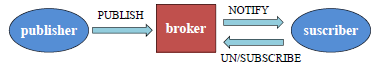
\includegraphics[width=80mm]{img/publishsub.PNG}
\caption{Paradigma publish-subscribe}
\label{fig:pps}
\end{figure}
\bigbreak
\noindent I publisher e i subscriber non si parlano direttamente, c'è il broker di mezzo. \\ Il broker può essere decentralizzato o centralizzato: in linea ipotetica ogni nodo della rete può essere broker, viene creato una rete che si auto-organizza in cui i nodi cooperano per portare le informazioni dove sono richieste. 
\bigbreak
\noindent Il broker permette disaccoppiamento di tre tipi:
\begin{itemize}
    \item [-] spaziale: le parti interagenti (publisher e subscriber) non hanno bisogno di conoscere né il numero né l'identità delle altre parti (utile in challenged net in cui i nodi devono fare economia spegnendosi, o obbedire ad un duty cicle)
    \item [-] temporale: non c'è bisogno che un publisher e un subscriber siano contemporaneamente presenti nella rete (il dato resta in pancia al broker). Il publisher produce/subscriber consuma dato anche mentre l'altra parte è disconnessa. Punto di rottura con la comunicazione sincrona di Internet. 
    \item [-] di sincronizzazione: publisher che produce un contenuto non è bloccato in attesa che qualche subscriber lo consumi. 
\end{itemize}
Il paradigma pub/sub è adatto per ambienti mobili e reti challenged: permettono ai nodi, che devono risparmiare batteria, di spegnersi lasciando la rete e di ricollegarsi quando si riaccendono senza che la rete ne sia inficiata. Inoltre reti challenged, come reti di sensori, possono essere formati da molti nodi, il disaccoppiamento spaziale facilita la partecipazione di molti nodi. 
\bigbreak
\noindent \textbf{Topic-based publish-subscribe} \\
Gli argomenti dei contenuti sono etichettati a seconda del topic, ogni topic è identificato da una stringa. I topic possono essere organizzati in una tassonomia. Sottoscrivere un topic è come sottoscrivere un gruppo (tutti i suoi sub-topic, sottogruppi), attenzione alla granularità (ex. al subscriber interessa il topic "temperatura", gli vengono inoltrati i messaggi riguardanti questo topic ed è il subscriber a fare un controllo sul messaggio, guardando se la temperatura è sotto una certa soglia e accendendosi di conseguenza)
\bigbreak
\noindent \textbf{Content-based publish-subscribe} \\
Sottoscrivo un insieme di contenuti caratterizzati da certe proprietà, cioè eventi per cui una certa asserzione è vera (meta-dati). Il broker non fa un matching di stringhe di topic come sopra, in questo caso il broker guarda dentro i contenuti, deve processarli e capirne le proprietà. Fa poi matching con le proprietà richieste dai subscriber (ex. il broker apre i messaggi e li inoltra ai subscriber solo se la temperatura è minore di una certa soglia).
Il problema è aggiungere intelligenza al broker
\bigbreak
\noindent \textbf{Type-based publish-subscribe} \\
Il subscriber specifica di voler ricevere oggetti che hanno una determinata struttura (ex. i publisher sono device utente o sensori ambientali, il subscriber vuole ricevere solo oggetti della classe "sensore" e non "user device", perché vuole regolare la temperatura in base ai sensori e non alla preferenze utente. Il subscriber sottoscrive la classe sensore).
\bigbreak
\noindent \textbf{Confronto}:
\begin{enumerate}
    \item I topic devono essere predefiniti, se aderisco ad un gruppo troppo generico ricevo troppo traffico. Altrimenti il subscriber deve aderire a gruppi più specifici, ma aumentiamo la complessità di computazione (il broker ci mette più tempo a fare matching e deve tenere traccia di molti dati per ogni subscriber)
    \item type è simile al topic ma è più facile da implementare. Usiamo tipi che già usavamo in progettazione, il problema è che nel momento in cui devo rilasciare una release del SW, magari devo andare a toccare molti aspetti del SW.
    \item content è la più flessibile. E' granulare quanto desidera, basta specificare che asserzione dev'essere vera per ogni evento. Non poniamo vincoli su etichette o strutture dati predefinite per ogni evento. Nel content-based arrivano solo le informazioni di interesse.
\end{enumerate}

\chapter{Wireless Sensor Network (WSN)}
\label{cap:wsn}
Bibliografia - si trovano in lezione e materiali didattici: 
\begin{itemize}
    \item[-] I. Akyildiz, W. Su, Y. Sankarasubramaniam, \textit{“Wireless
            Sensor Networks: A Survey”}.
    \item[-] J. Elson, D. Estrin, \textit{“Wireless Sensor Networks: a bridge to
            the physical world”}. (solo lettura)
\end{itemize}

\begin{figure}[h]
	\centering
    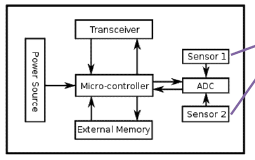
\includegraphics[width=55mm]{img/sensore.PNG}
    \caption{Oggetto sensore}
    \label{fig:se}
\end{figure}

\noindent In figura c'è un "sensore oggetto (board)":
\begin{itemize}
    \item ADC (Analog to Digital Converter): un sensore spesso esegue misure di grandezze analogiche, abbiamo bisogno di convertirle. Una volta convertire vengono passare al microcontroller.
    \item Microcontroller: è la CPU. C'è una memoria esterna dove viene salvato anche il codice eseguibile. Esso controlla le comunicazioni ed è alimentato da una sorgente di energia. 
    \item Sensori veri e propri: apparato in grado di rilevare e quantificare segnali dal mondo fisico in cui è immerso (sensor 1 e sensor 2)

\end{itemize}

\noindent Esistono tre categorie di sensori "veri e propri":
\begin{itemize}
    \item [-] passivi omnidirezionali: non agiscono sul mondo circostante, possono osservare grandezze del mondo fisico da qualsiasi direzione essa provenga (la temperatura, il suono lo misuro da qualunque direzione provenga)
    \item [-] passivi unidirezionali: non agiscono sul mondo circostante, ma misurano una grandezza in una sola direzione (videocamera)
    \item [-] attivi: per misurare il mondo circostante, agiscono su di esso (sonar/radar che verificano la presenza di oggetti emettendo ultrasuoni/onde)
\end{itemize}


\noindent \textbf{Attuatori}: dispositivo che non misura niente, ma che riceve comandi per modificare l'ambiente in cui è immerso (ex. il campo è asciutto, ricevono il comando di far partire l'irrigazione). \\ 
\textbf{Sink}: punto di raccolta delle informazioni rilevate dai sensori. I sink sono normalmente connessi alla rete elettrica e ad Internet. Essi raccolgono i dati, possono elaborarli direttamente oppure parzialmente inoltrandoli poi ad un altro nodo. \\
\textbf{Coordinatore}: capiscono come funziona il mondo processando i dati dei sensori, i coordinatori hanno intelligenza e riconfigurano il funzionamento dei sensori (cambiando la grandezza da misurare, oppure aumentando la frequenza di campionamento). 

\section{WSN caratteristiche}
\label{sec:WSNcar}
Wireless Sensor Network è una qualunque infrastruttura di rete in cui sono presenti oggetti classificabili come sensori, attuatori, sink, coordinatori. \\ Non ci sono architetture o soluzioni standard, si studiano da relativamente poco e sono molti i casi applicativi nei quali sono utilizzabili. 
\bigbreak
Gli apparati che formano le WSN possono essere molto piccoli, per essere pervasivi, questo comporta che siano fragili, facilmente spostabili e computazionalmente limitati. Sono anche oggetti che non necessitano grandi quantità di energia, le comunicazioni sono a corto raggio. 
\bigbreak
Per quanto riguarda l'alimentazione, possono essere alimentati o meno. Sono alimentati se si trovano in un ambiente che offre la possibilità di connessione elettrica, nel caso non sia possibile alimentarli, si possono usare delle batterie oppure fare "energy harvesting", tentativo di trarre energia dall'ambiente circostante (ad ex. celle solari): i sensori sono distribuiti sul territorio da monitorare e può essere difficile raggiungerli, guasti o esaurimento di energia non sono risolvibili. \\ Questi oggetti sono muniti di un'interfaccia wireless per la comunicazione, se ci sono un numero enorme di sensori non posso cablare tutta la zona interessata. 
\bigbreak
Una difficoltà/opportunità è di poter costruire la rete con apparati differenti, con capacità di computazione diverse, con radio e interfacce di rete differenti in tecnologia usata e in potenza. Ad ex. alcuni apparati usano NFC, comunicano a distanza di centimetri trasmettendo byte, altri apparati hanno risorse sufficienti per essere equipaggiate di interfaccia WiFi. Dobbiamo fare in modo che, questi apparati diversi, possano comunicare e capirsi: usiamo dei gateway, qualche oggetto che abbia entrambe le interfacce e che sia in grado di prendere dati da un'interfaccia, trasformarne il formato a seconda dei protocolli usati, e trasferirli all'altra interfaccia. Aumento in complessità, ma anche un'opportunità per differenziare i compiti dei nodi. 
\bigbreak
\noindent \textbf{Multipath fading}
\bigbreak
\noindent Parliamo sempre di reti wireless, quindi prone ad interferenze di apparecchi che usano lo stesso range di frequenze e ad interferenze ambientali (ad ex. non posso aspettarmi che se metto due sensori nei due lati opposti di un muro in cemento armato, questo si sentano). Il segnale radio viaggia in linea retta, decadendo allontanandosi dalla sorgente, gli oggetti e le superfici in parte assorbono/bloccano il segnale, in parte lo riflettono. \textbf{Il multipath fading è l'interferenza causata dal segnale che interferisce con se stesso creando rumore, disturbando il segnale principale. }

\begin{figure}[h]
	\centering
    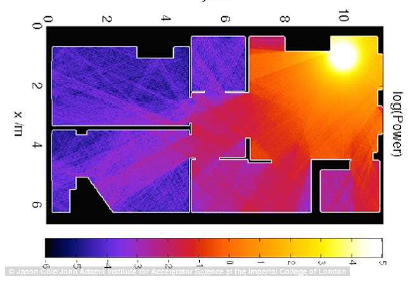
\includegraphics[width=85mm]{img/mpathfad.PNG}
    \caption{Multipath fading}
    \label{fig:mfad}
\end{figure}

All'esterno vale lo stesso, creano interferenza le auto, le gru, la radiazione luminosa (il sole emette un po' anche nello spettro delle onde radio). Ad ex. tentativo di far comunicare due caserme mettendo sui loro tetti delle antenne unidirezionali, la rete ha smesso di funzionare: le due antenne erano su tetti bitumati (nero), al sole erano diventati roventi. L'alta temperatura del tetto aumenta la temperatura dell'aria sopra, cioè l'energia delle particelle dell'aria soprastante. Questo ha disturbato il segnale tra le due antenne. 

\section{WSN requisiti}
\label{sec:WSNreq}

\begin{itemize}
    \item[-] \textbf{Accuratezza del monitoraggio}: i sensori devono garantirci con alta probabilità che saranno in grado di registrare gli eventi per i quali sono installati
    \item[-] \textbf{Autonomiche/self-organization}: operare correttamente, o sapersi riconfigurare, indipendente dalle condizioni ambientali e della presenza umana che possa aggiustare eventuali guasti della rete. 
    \item[-] \textbf{Risparmio energetico}: la comunicazione tra nodi è la componente principale di consumo energetico. 
    \bigbreak
    Ci sono diversi livelli di consumo energetico, un nodo può essere completamente accesso in ogni suo componente, oppure un nodo potrebbe essere spento consumando energia zero. Ci sono livelli intermedi: possiamo mettere a dormire quasi tutto il nodo (l'interfaccia radio è ferma, possiamo quasi fermare la CPU dando un duty cicle al nodo), oppure possiamo fermare la CPU ma con interfaccia radio sveglia, non manda nulla ma può sentire (se sente un messaggio rivolto a lui, risveglia il nodo). \\ Un nodo idle consuma il 10\% dell'energia che consumerebbe per ricevere dati e il 5\% dell'energia che impiegherebbe per inviarli.  
    \item[-] \textbf{Lifetime sensori e rete}: dobbiamo considerare il ciclo di vita sia della rete che dei singoli sensori. Il ciclo di vita della rete deve durare più a lungo possibile, non è detto che ciò vada di pari passo con la durata di un singolo sensore (il nodo egoisticamente si sveglia solo quando riceve un messaggio per lui, ma non aiuta a fare inoltro di pacchetti verso gli altri nodi, ciò massimizza la vita del nodo ma non della rete). 
    \item[-] \textbf{Scalabilità}: costo del sistema in relazione al numero delle sue componenti. Ho una moltitudine di nodi, spesso molto vicini tra loro, le soluzioni SW devono essere in grado di gestirla. 
    \item[-] \textbf{Robustezza}: i nodi possono operare in ambienti ostili, ma accuratezza e lifetime devono essere preservati. Gracefull degradation: la rete è messa giù bene, nel tempo si possono verificare problemi di ogni tipo, la GD mi dice che le prestazioni della rete dovrebbero decadere in modo dolce. 
    \item[-] \textbf{Consenso}: coordinamento tra i sensori. Questo serve perché quello che ci viene detto da un solo sensore potrebbe non essere significativo e non affidabile. 
\end{itemize}

\section{Deployed vs Unplanned}
\label{sec:depunp}
\noindent \textbf{Reti di sensori deployed}: gli oggetti che ne fanno parte sono più grandi dell'ordine dei centimetri e sono posizionati singolarmente in punti predeterminati.
\bigbreak
\noindent \textbf{Reti di sensori unplanned}: gli oggetti sono molto piccoli, nell'ordine dei centimetri, non possiamo collocare singolarmente ogni sensore, vengono sparpagliati. 

\begin{figure}[h]
	\centering
    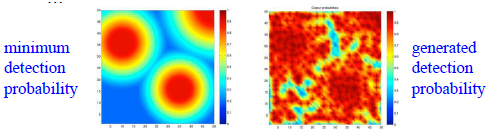
\includegraphics[width=85mm]{img/depun.PNG}
    \caption{Deployed-unplanned}
    \label{fig:du}
\end{figure}

Figura di sinistra: è visualizzato il quadrato di area che vogliamo misurare ed è utile a visualizzare l'accuratezza del monitoraggio. Il colore di ogni punto indica la probabilità con cui vogliamo essere capaci di rilevare un evento se si verifica in quel punto (in un'area di colore blu ho intorno al 15\% di probabilità di validare l'evento).
Nelle reti deployed questa mappa guida il posizionamento dei sensori, è un problema di ottimizzazione che tiene conto di molte variabili (costo, quanti sensori, accuratezza, robustezza, lifetime.
\bigbreak
Figura di destra: notiamo che i punti più scuri sono i nodi e che c'è corrispondenza di colori e zone tra le due figure. Ma ci sono anche differenze: l'angolo in basso a sinistra? Sono stati aggiunti dei nodi non per effettuare misurazione in zone che prima non erano coperte, che probabilmente quindi non mi interessavano, ma per creare dei path alternativi tra le chiazze, gruppi di sensori per permettere maggior passaggio di informazioni tra i nodi della rete. 

\section{Posizione e sincronizzazione}
\label{sec:possinc}
\noindent\textbf{Location awareness} \\
Se gli oggetti, sensori o attuatori, sono deployed possiamo fare un passaggio ulteriore: carico su ogni oggetto la sua posizione, che conosco. In una rete unplanned questo non è possibile, nel momento in cui sparpaglio non so dove cade il sensore, e la posizione devo ricavarla in qualche modo. L'informazione di locazione ci serve ad ex. se tutti i sensori in una stanza indicano che c'è del fumo e del caldo, probabilmente ci sarà un incendio. L'informazione di locazione contribuisce all'aggregazione di dati, permettendoci di capire meglio il fenomeno. 
\bigbreak
Il metodo più facile è il GPS. GPS funziona solo outdoor perché usa un segnale radio debole che si interrompe quando incontra muri. GPS usa anche molta batteria, non riesco a massimizzare il lifetime della rete. 
\bigbreak
Vedremo più avanti utilità e tecniche, tecniche per cui una rete unplanned può capire dove si trovano i sensori e protocolli che sfruttano la posizione per funzionare.
\bigbreak
\noindent\textbf{Localizzazione e sincronizzazione} 
\begin{figure}[h]
	\centering
    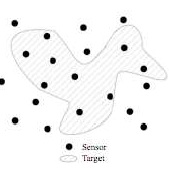
\includegraphics[width=40mm]{img/locsinc.PNG}
    \caption{Localizzazione e sincro}
    \label{fig:locsin}
\end{figure}

\noindent In figura: l'area tratteggiata è quella in cui sta succedendo un evento, i punti neri sono i sensori che sono in grado di rilevare quell'evento. Può essere importante che i nodi sappiano dove sono: ho un insieme di nodi dentro all'area tratteggiata, questi sanno capire se sta accadendo qualcosa e in che area questo succede (ex. sono nella zona del Chianti ho dei sensori che mi dicono quando irrorare il terreno, ma se non conosco la posizione dei sensori non so che specifica zona risulta secca). 
\bigbreak
\textbf{La conoscenza della posizione può servire per attivare sensori nell'area target di interesse, questo ci da informazioni sull'evento, sulla sua estensione. Può anche indicarci se l'evento si stia muovendo o allargando.} \\

In una rete unplanned non ho idea di quali siano gli indirizzi MAC e le posizioni dei nodi, approccio data-centric: mando un messaggio a tutti i sensori intorno all'area di interesse. 
\bigbreak
\noindent\textbf{Sincronizzazione clock}
\bigbreak
Serve per dire cosa si verifica prima o dopo, per capire se un evento si sta spostando e in che direzione (ad ex. un sensore in coordinate (x1, y1) rileva fumo alle 22:00, un altro sensore in (x2, y2) lo rileva alle 22:02. Posso dire che il possibile incendio si sta spostando in direzione (x2, y2)). \\
Avendo informazioni riguardo alla posizione e agli orari, è possibile anche determinare a che velocità si sposta l'evento. \\
\bigbreak
\noindent \textbf{Naming e routing} \\
Se le reti sono unplanned non abbiamo idea di quale nodo, in indirizzo MAC, sia in determinate coordinate. 

\noindent Non c'è naming dei sensori, soprattutto nelle reti unplanned, viene fatto un routing data-centrico: non è routing come in Internet, non potendo andare ad un determinato indirizzo, diffondo la direttiva ai solo sensori in grado di verificare l'evento a cui sono interessato. 
\bigbreak
Vengono effettuate query che non sono dirette ad un nodo, ma al dato (dato-centriche): è un'informazione importante per nodi che montano uno specifico sensore, indipendente dalla loro posizione (ad ex. segnalatemi quando la temperatura supera i 40°). 
\bigbreak
Le query vanno dal sink ai sensori, dai sensori al sink vanno le notifiche di eventi (dettate dal sink o dal codice interno del sensore). La comunicazione va dal coordinatore, controllore ai sensori o attuatori, ma non il contrario. Queste parti si cercano uno con l'altra senza sapere direttamente l'indirizzo.
\bigbreak
\noindent \textbf{Range di comunicazione} \\
Le onde radio viaggiano in linea retta e i dispositivi per sentirsi devono essere nei propri raggi di comunicazione e allineati (line-of-sight: posso vedere la sorgente perché non vi sono ostacoli). La potenza del segnale va circa con il quadrato della distanza $1/d^2$, nel punto in cui c'è la sorgente la potenza è massima.
\begin{figure}[h]
	\centering
    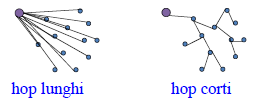
\includegraphics[width=60mm]{img/range.PNG}
    \caption{Hop}
    \label{fig:hops}
\end{figure}
\bigbreak
In figura: il pallino più grosso è il sink, quelli piccoli sono i sensori. I sink e i nodi sono nelle stesse posizioni, cambia la topologia della rete.
\bigbreak
Figura sx - hop lunghi: ogni sensore è stato collegato con un arco che arriva direttamente al sink, ogni sensore sa comunicare direttamente con il sink. Ci sono sensori più vicini al sink e altri più periferici, i sensori più lontani devono usare molta più potenza per comunicare, e quindi più energia esaurendo prima la loro batteria. Potrebbe non essere una buona idea. Inoltre il sensore parla con il sink con un hop solo, se è presente un ostacolo in mezzo non c'è modo di poterlo aggirare. 
\bigbreak
Figura dx - hop corti: i sensori parlano con sensori vicini e utilizzando piccoli-hop, costruisco una struttura che connette tutti i sensori al mio sink. I sensori devono farsi sentire a distanza breve, usando poca energia: la comunicazione costa meno e la vita dei sensori, vicini o periferici, dura di più. Nel caso ci siano ostacoli che impediscono le comunicazioni, è possibile trovare un path alternativo per poterlo aggirare. 
\bigbreak
Un nodo genitore dell'albero deve inoltrare i messaggi di tutti i suoi figli e il proprio verso il sink. In figura c'è un unico sensore che riesce a parlare direttamente con il sink, deve inoltrare i messaggi di tutti gli altri nodi. E' possibile che sensori più vicini al sink terminino prima la loro batteria, rendendo la rete quasi inutile. Per risolvere facciamo \textbf{data aggregation con ottimizzazione}: mettiamo insieme informazioni provenienti da più sensori. Scegliamo nodi che pagano meno per ricevere che per trasmettere, un nodo genitore riceve i dati dai suoi nodi figli, fa lui una considerazione dell'ambiente (ad ex. valore medio e varianza dei dati ricevuti) e manda solo un valore. Aggiungo un pre-processing parziale nella rete, il sink non riceve direttamente raw-data. 
\bigbreak
\noindent Solitamente si scelgono hop corti:
\begin{itemize}
    \item migliore distribuzione del lavoro tra sensori (vicini, periferici tutti parlano ad intensità minore)
    \item durata più omogenea dei sensori e della rete
    \item possibile effettuare data aggregation con ottimizzazione
\end{itemize}
Problema con gli hop corti: devo individuare un grafo che consenta di portare informazioni al sink: i sensori devono conoscere la loro posizione rispetto al sink e la posizione del sink, quindi serve la conoscenza delle posizioni per il routing. 
\bigbreak 
Potrebbe essere che un sensore non ricevi risposte da nessun sensore nei suoi paraggi, possiamo decidere che il sensore aumenti il suo raggio di comunicazioni nel caso non senta vicini intorno a se. Bisogna progettare questa tipologia di rete partendo dall'HW, che deve permettere il variare dell'intensità del segnale. 

\section{Data aggregation}
\label{sec:dagg}

La stessa segnalazione può arrivare da più sensori (ho tre webcam per la sorveglianza, tutte e tre vedono un ladro. Il sink riceve i dati, ma non sa se sono tre ladri diversi o lo stesso). Potrebbe essere che il sink riceva troppi dati non riuscendo a processarli oppure che l'antenna del sink riceva molti segnali, e quindi che alcuni di essi si annullino o si disturbino a vicenda. 
\bigbreak
Se uno stesso evento è monitorato da più sensori, possiamo decidere di effettuare del pre-processing: aggreghiamo dati di più sensori e mandiamo un solo messaggio al sink. 
\begin{itemize}
    \item non sovraccarico il sink
    \item elimino ridondanza
    \item non passo informazioni non molto utili
\end{itemize}

\noindent Il pre-processing in rete è utile per:
\begin{itemize}
    \item Ci sono meno trasmissioni, evitano collisioni sul canale wireless e non sovraccaricano il sink. Aumento la robustezza e l'affidabilità della comunicazione, viaggiano meno dati che non si disturbano reciprocamente. 
    \item In ogni dato non metto tutte le rilevazioni dei miei sensori figli, metto solo media e varianza
    \item trasmetto per meno tempo, risparmia la batteria del nodo e intaso meno la rete
    \item Meno contesa sul mezzo
    \item Risparmio energetico: fare pre-processing mi richiede aggiungere intelligenza sull'apparecchio e farli computare run-time. Tuttavia il consumo massimo d'energia lo sfrutto per la comunicazione. 
    \item I nodi devono sapere aggregare: all'interno della rete, quando faccio routing verso il sink e i nodi intermedi fanno aggregation (nodi che potrebbero non aver osservato l'evento, devono solo fare routing di notifiche iniziate da altre) devono capire cosa fare con i dati che ricevono, che è molto legato al livello applicazione. 
\end{itemize}

Altri aspetti che dobbiamo considerare nella costruzione di una rete:
\begin{itemize}
    \item Database: vengono raccolti, aggregati dati dai sensori, è possibile che vengano usati dei DB. Sono DB non relazionali, con requisiti di prestazioni particolari, che sanno gestire dati real-time. E' un DB distribuito, ogni nodo si tiene poche informazioni - proprie o che ha sentito dai vicini. Comporta dei problemi: è difficile per il sink effettuare una query (ex. temperatura media delle ultime 3 ore, che comunque viene effettuato con query data-centric) ed è difficile per i sensori convogliare tutte le informazioni in un punto centrale. 
    \item sicurezza: le informazioni sono passate in un mezzo wireless e possono essere captati. E' possibile usare degli algoritmi di cifratura ma devono essere molto leggeri. Ci dev'essere anche consenso su un insieme di valori, ci sono algoritmi che cercano di far prevalere il valore dei nodi onesti, cercando di non ascoltare nodi maligni.
    \item attuatori: gli attuatori possono influenzare le misurazioni dei sensori. I sensori rilevano eventi in una zona, mandano tutto al sink e poi al coordinatore. Il coordinatore comunica agli attuatori di spostare dei sensori verso la zona interessata, in modo da campionarla più densamente (i sensori devono essere mobili)
\end{itemize}

\section{Nodi statici vs Nodi mobili}
\label{sec:nsnb}
\noindent \textbf{Ferries}: nodi di cui possiamo controllare il movimento, gli attuatori possono ordinargli di spostarsi. Se abbiamo delle partizioni di rete, il ferrie si può spostare in un gruppo di nodi isolati, il ferrie carica nella propria memoria i dati raccolti dal gruppo e, spostandosi, lo riporta ad un altro gruppo di nodi o al sink. \\ I ferries possono anche essere mobili ma non controllabili, radio-collari sulla fauna. In questi casi potrei individuare delle regolarità negli spostamenti degli animali, dei veicoli e servirmene per portare informazioni nelle varie zone della rete (mi servono studi sui pattern di mobilità). 

\section{Architetture gerarchiche}
\label{sec:ag}
Torniamo all'eterogeneità dei nodi all'interno delle reti challenged. \\ L'insieme di lavori possibili (sensing ambientale, computazione, attuazione) non è fatto omogeneamente da tutti, perché ognuno ha capacità diverse, posso creare una gerarchia.
\bigbreak
\noindent \textbf{Three-tired Architecture}: 
\begin{enumerate}
    \item un livello è molto semplice, formato da apparecchi poveri di risorse, poco costosi e quindi ne posso avere molti (sensori). Poca energia, poca potenza di calcolo e memoria, spesso sono messi in modo unplanned.
    \item il secondo livello ha apparecchi (microserver) con più capacità. I microserver/aggregatori sono più costosi, alimentati con batterie potenti e con potenza di calcolo non male. Sono spesso comprati in numero limitati e sono deployed, ogni sotto-area della WSN ha un microserver. Probabilmente sono dei gateway: interfaccia wireless a corto raggio per ricevere i dati dei sensori e interfaccia wireless a raggio più ampio per inoltrare i dati ad un altro microserver o a un sink. 
    \item l'ultimo livello è Internet, è wired, c'è tutta la potenza di calcolo e memoria che desidero (infrastruttura cloud o EDGE server). 
\end{enumerate}

\begin{figure}[h]
	\centering
    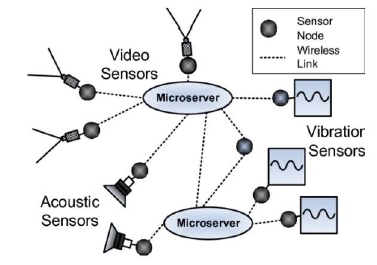
\includegraphics[width=70mm]{img/3tier.PNG}
    \caption{Esempio di rete 3-tier}
    \label{fig:3t}
\end{figure}

\chapter{Direct Rumor}
\label{cap:dr}
Materiale - si trovano in lezione e materiali didattici: 
\begin{itemize}
    \item[-] C.Intanagonwiwat, R. Govindan, D. Estrin, \textit{Directed
            Diffusion: a scalable and robust communication paradigm
            for sensor networks}
    \item[-] D. Braginsky, D. Estrin, \textit{Rumor Routing algorithm for
            sensor networks}
\end{itemize}
\noindent \textbf{Assunzioni su entrambi i metodi} \\ WSN unplanned: reti dense con tanti nodi vicini tra di loro per garantire accuratezza della copertura e aumentare la probabilità che la rete non sia partizionata. Sono nodi che non si muovono e usano algoritmi di routing data-centric. 
 \begin{itemize}
     \item[-] distribuzione unplanned
     \item[-] non sfruttano posizione per fare routing
     \item[-] sensori hanno un ID (indirizzo, numero fittizio) e hanno orologi sincronizzati (non è per il funzionamento degli algoritmi di instradamento ma usata per dare più significato al dato letto dal sensore)
     \item[-] non c'è mobilità, la rete è densa (topologia è molto connessa, molti cammini)
     \item[-] i sensori sono in grado di fare un minimo di computazione (ad ex. calcolo media, minimo, massimo, varianza)
     \item[-] canale wireless (possibili collisioni tra trasmissioni simultanee, mezzo trasmissivo non isolato e quindi interferenze. Comunicazioni non affidabile).
     \item[-] preferiti gli hop corti.
 \end{itemize}

\section{Reverse path forwarding}
\label{sec:erp}
Parte dal fatto che il sink comunica alla rete che vuole ricevere informazioni dai sensori sul verificarsi di un determinato evento. Nella propagazione di questa richiesta, il sink costruisce dei cammini tra sé e i sensori. Nel momento in cui il sensore riceve la richiesta, sfrutta all'indietro il cammino  che è stato individuato dal sink ai sensori per comunicare il verificarsi dell'evento. 
\bigbreak
E' un servizio pull (affine a client HTTP che chiede cose al server), il destinatario sink chiede un servizio ai sensori sorgenti (chi genera dati) per ricevere certe informazioni. 
\bigbreak
\subsection{Directed Diffusion}
\label{sec:dd}
\noindent Applica un paradigma Reverse Path Forwarding. \\ Tutto parte da un interest del sink, se il sink non comunica nulla, i sensori non fanno nulla. 

\begin{figure}[h]
	\centering
    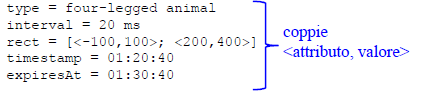
\includegraphics[width=95mm]{img/dd.PNG}
    \caption{Esempio di interest}
    \label{fig:exint}
\end{figure}

Al sink interessa il passaggio di un animale in un dato rettangolo con coordinate $<-100, 100> <200, 400>$ fino al momento 01:30:40. \\ La posizione e l'ora non vengono usati per routing, nell'esempio sono usati dal sensore per capire se si trova all'interno del rettangolo desiderato nell'ora richiesta.

\begin{figure}[h]
	\centering
    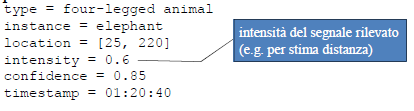
\includegraphics[width=95mm]{img/dd2.PNG}
    \caption{Esempio di risposta del sensore}
    \label{fig:exsens}
\end{figure}

Un sensore è stato messo in allerta dall'interest, il sensore vede di essere in quel rettangolo e sa di essere in grado di capire se ci sono animali, allora capisce di doverlo comunicare al sink. Il sensore manda una descrizione di evento, in figura. Il sensore specifica anche il tipo di animale, la posizione, l'intensità, l'intervallo di confidenza e il timestamp (momento in cui il sensore ha osservato l'evento). 
\bigbreak
\noindent \textbf{Caratteristiche di Directed Diffusion}
\begin{itemize}
    \item WSN piatta: non 3-tier, tutti i nodi hanno stesse funzionalità, rete unplanned.
    \item canali bi-direzionali 
    \item routing reattivo (i router di Internet ogni tot tempo scambiano le informazioni sui propri vicini per mantenere le tabelle di instradamento, in DD costruiamo cammini solo se dobbiamo mandarci sopra qualcosa) 
    \item interest diffuso in flooding (il sink manda l'interest a tutti i sensori nel suo raggio radio e ogni sensore che lo sente, lo manda a tutti i suoi vicini). 
    \item durante il funzionamento, DD cerca di individuare i cammini migliori in reverse path da sensori a sink. E' permesso mantenere cammini multipli, mi ricordo il migliore ma ne ricordo anche altri, nel caso non fosse disponibile. C'è anche la possibilità di cercare di aggirare punti problematici (sensore scarico, ostacolo tra sensori) per trovare un cammino alternativo. 
    \item i sensori riescono a fare pre-processing: aggregano dati negli hop intermedi. 
    \item DD risparmia energia, i sensori lavorano quando interpellati dal sink.
    \item si formano loop (ridondanza che ci aiuta, aumenta robustezza della rete)
\end{itemize}
\bigbreak
\noindent \textbf{Diffusione dell'interest} 
\bigbreak
\noindent Ogni sink - possono essercene più di uno - costruisce un interest, e finché l'interest è attivo (\textit{fino a expires at}) viene mandato periodicamente in broadcast ai sensori nel raggio radio del sink. Viene fatto periodicamente per affidabilità: i sensori potrebbero essere spenti e accendersi ogni tot per verificare se ci sono interest oppure, pagando di più in termini di energia, potrebbero lasciare accesa l'antenna radio e svegliandosi se sentono interest. Inviare periodicamente in broadcast permette, nel primo caso, di beccare il sensore quando è sveglio, oppure di rimediare se c'era interferenza. 
\bigbreak
Con la prima diffusione di interest, il sink comunica ai sensori un intervallo di campionamento ampio: il sink non sa se l'evento si verificherà, chiedere ai sensori di accendersi e campionare frequentemente comporta una perdita di batteria. Se il sink riceve informazioni sul verificarsi dell'evento, può mandare un altro interest aumentando la frequenza di campionamento dei sensori. Ogni nodo che riceve un interest lo ricorda nella cache
\begin{figure}[h]
	\centering
    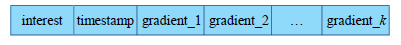
\includegraphics[width=90mm]{img/interest.PNG}
\end{figure}
\bigbreak
C'è un campo gradiente, ma non c'entra con cost-filed. Questi gradienti ci indicano il vicino one-hop dal quale il nodo ha ricevuto l'interest. Non ho idea se questo vicino sia il sink, un nodo vicino o lontano 40 hop dal sink, sa solo che se deve ridare la risposta al sink deve seguire quel cammino. \\ Ci sono k gradienti perché lo stesso interest mi può arrivare da più vicini, questo a causa del flooding. \\ Dei nodi vicini mi ricordo ID, mi ricordo quanto tempo dura l'interest arrivato e il data rate, cioè ogni quanto il sink vuole avere una notifica \\ ($<$ data rate, duration, neighbor ID $>$) 
\bigbreak
\noindent \textbf{Differenti metodologie di re-inoltro degli interest} 
\begin{figure}[h]
     \centering
     \begin{subfigure}[b]{0.3\textwidth}
         \centering
         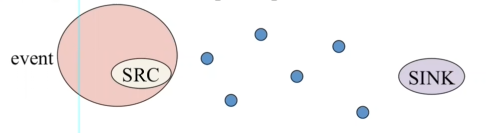
\includegraphics[width=40mm]{img/r1.PNG}
         \caption{Step 1}
     \end{subfigure}
     \hfill
     \begin{subfigure}[b]{0.3\textwidth}
         \centering
          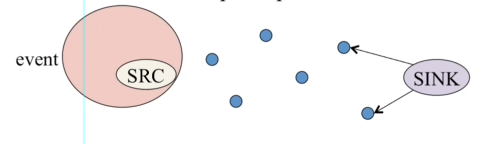
\includegraphics[width=40mm]{img/r2.PNG}
          \caption{Step 2}
     \end{subfigure}
     \hfill
     \begin{subfigure}[b]{0.3\textwidth}
         \centering
         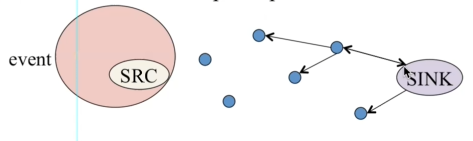
\includegraphics[width=40mm]{img/r3.PNG}
         \caption{Step 3}
     \end{subfigure}
     
    \caption{Primi step del flooding}
    \label{fig:flood}
    
\end{figure}
    
\begin{enumerate}
    \item \textbf{Flooding}: il sink manda in broadcast l'interest ai suoi vicini, i vicini re-inoltrano solo se l'interest non è duplicato e non è stato inoltrato recentemente (re-inoltro ogni tanto per beccare vicini prima non attivi e non troppo spesso per risparmiare energia). 
    In figura \ref{fig:flood} (c) notiamo che il nodo in alto ha re-inoltrato a tutti i suoi vicini, compreso il sink (il nodo non sa se l'interest è stato ricevuto dal sink o da un nodo comune, inoltre è utile per la costruzione di cammini. In secondo luogo è una sorta di ACK, il nodo predecessore sa che l'interest è stato preso in carico anche da qualcun' altro). 
    
    \begin{figure}[h]
	\centering
    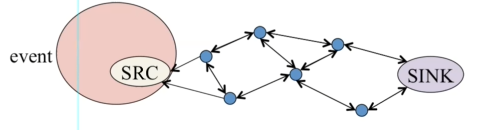
\includegraphics[width=80mm]{img/r4.PNG}
    \caption{grafo finale flooding}
    \label{fig:grflood}
    \end{figure}

    Il grafo ci indica che abbiamo una grande quantità di percorsi possibili, le frecce sono tutte bi-direzionali, questo per ora è comodo. \\
    Problemi: $O(n^2)$ in termini di costo, inoltre vengono mandati messaggi a vicini del sink che non sono nemmeno in direzione dell'evento, occupando banda e spendendo in energia. 
    \item \textbf{Routing geografico verso area target}: se c'è qualche nozione di posizione, i nodi intermedi potrebbe sfruttarla per inoltrare l'interest verso l'area di interesse. Vedremo più avanti. 
    \item \textbf{Direzione cached da risposte precedenti}: se non abbiamo nozioni geografiche, il sink e i nodi intermedi si possono ricordare che in precedenza un interest analogo era già stato spedito. Invece di fare flooding, faccio un broadcast limitato, un multicast, verso un sottoinsieme di vicini che mi hanno fornito risposte per un interest simile. Non è banale, dobbiamo aggiungere memoria e intelligenza nei nodi (devono ricordare che interest sono passati, chi ha risposto e intelligenza necessaria a capire l'anologia tra interest passato e presente). 
\end{enumerate}

\noindent \textbf{Routing delle notifiche di eventi} \\
I gradienti indicano i vicini one-hop che sono interessati all'evento, c'è ridondanza di gradienti (robustezza e repair e per inoltrare verso più sink con il medesimo interest). 
\bigbreak
Un sensore dentro l'area di interesse riceve tre interest con frequenza di campionamento diverso, quanto si sveglia il sensore? Il sensore sceglie la frequenza più alta, soddisfando il sink che ha requisiti più stringenti e di conseguenza anche gli altri, $max(datarate-gradienti)$. Questo non implica che mando notifiche a campionamento alto a tutti i gradienti, rispetto le frequenze richieste da ciascuno (1, 3, 5 minuti - campiono ogni 1 minuto ma non mando a tutti e tre i dati ogni minuto, mando al secondo gradiente ogni tre e al terzo ogni cinque minuti).
\bigbreak
\textit{Esempio di aggregazione di dati: se un nodo, sink o intermedio, riceve un report su un evento più frequentemente del data rate di qualche suo gradiente (un nodo ha due gradienti, uno chiede report ogni minuto e l'altro ogni tre. Il nodo esaurisce la richiesta con il vincolo più stringente inoltrando una notifica ogni minuto, mentre manda un report ogni tre/la media dei tre, al secondo gradiente con data-rate meno frequente).}
\bigbreak
Quando si verifica l'evento mando una notifica a tutti i miei vicini e uso un indirizzamento uni-cast (mando un frame con nell'header l'indirizzo del vicino: non risveglio tutti gli altri vicini nel mio raggio radio non interessati a ricevere una notifica e non risveglio i vicini che non sono interessati a riceverla così spesso). I vicini potrebbero essere spenti eccetto per l'antenna radio, la scheda radio controlla se nell'header c'è il proprio MAC address e - nel caso - si sveglia (posso non svegliare gli altri sensori, risparmiando energia). 
\bigbreak
L'evento è ricordato in cache, se ricevono dei duplicati di notifica di evento non vengono re-inoltrati.
\bigbreak
La notifica di evento parte dal sensore nell'area di interesse, passa a tutti i gradienti del nodo che lo re-inoltrano. Nell'immagine ci sono linee tratteggiate: il nodo riceve un duplicato, si comporta come se tagliasse il cammino e non considera il doppione. 
\begin{figure}[h]
\centering
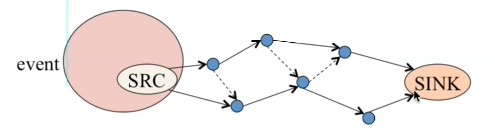
\includegraphics[width=80mm]{img/r5.PNG}
\caption{propagazione notifica evento}
\label{fig:evento}
\end{figure}
Quando scade la durata del gradiente, cancello il gradiente, interrompendo il cammino creato perché il gradiente non è più interessato all'evento. 
\bigbreak
\noindent \textbf{Rinforzo positivo} \\
Quando il sink inizia a riceve notifiche di eventi, può darsi che le riceva prima da un path che dall'altro, oppure le riceve da un vicino con un segnale più forte, meno interferenze, minor bit-error-rate. Il sink può rinforzare positivamente il vicino più conveniente dal quale riceve le notifiche: lo fa mandando, solo al nodo vicino che intende rinforzare, un interest con intervallo di tempo minore rispetto al primo messaggio (il primo interest è esplorativo, il sink non sa se l'evento si verificherà mai). Il rinforzo può proseguire a cascata, fino ai sensori nella zona interessata. Questi nodi cambiano il proprio data-rate di campionamento e mandano notifiche solo ai gradienti "rinforzati" dai quali hanno ricevuto la richiesta. \\ I nodi che non sono stati rinforzati, mantengono in cache in gradienti fino al tempo di \textit{expiresat}, è utile averli nel caso si rompesse il cammino rinforzato: ci sarà un momento di silenzio, dopo di che il sink inizierà a ricevere da un altro suo nodo vicino, a questo punto il sink rinforzerà questo nuovo nodo. \\ In alternativa, il sink può risparmiare energia nei sensori che non sono stati rinforzati - downconvert e rinforzo negativo
\bigbreak
\noindent \textbf{Rinforzo negativo - downconvert} \\
Il sink può far risparmiare energia ai path meno usati in tre modi:
\begin{itemize}
    \item lascia scadere la richiesta (la duration) anche se l'evento sta succedendo (soft state - no costo)
    \item diminuisce il data-rate del cammino non preferito, il cammino rimane attivo (hard state, overhead controllo)
    \item potrebbe mandare un interest con\textit{expiresAt} = timestampattuale o \textit{interval} = 0, per dire al nodo che non gli interessa più ricevere da lui. 
\end{itemize}
\bigbreak
\noindent \textbf{Prestazioni} \\
\begin{figure}[h]
\centering
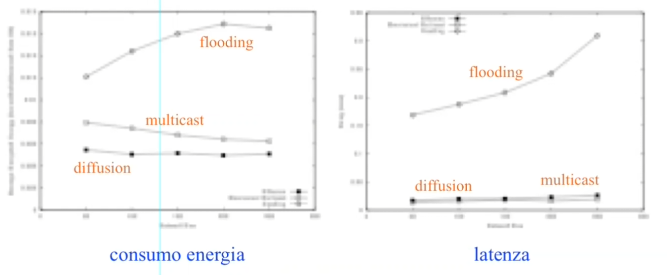
\includegraphics[width=93mm]{img/prestazion.PNG}
\caption{prestazioni metodi di propagazione notifiche}
\label{fig:pres}
\end{figure}
Sulle ascisse numero di nodi. \\
Figura sx: il flooding ha un consumo energetico maggiore, $O(n^2)$, quando i nodi sono tanti il flooding inizia a decrescere (avere tanti nodi comporta che i segnali interferiscano tra loro e alcuni nodi non ricevano e re-inoltrino i messaggi perché sono rumore. Il nodo che non riceve e non inoltra risparmia energia). Il multicast avviene calcolando i percorsi ottimi con l'algoritmo di Dijkstra inizialmente (i nodi sono fissi), è multicast perché un nodo potrebbe dover mandare una notifica a più sink. La differenza tra multicast e diffusion è data dall'aggregazione: un nodo che deve mandare la notifica verso più sink figli nell'albero ottimo, lo manda per tutto l'albero. In diffusion viene usato downconvert, se un gradiente ha un data-rate più basso gli viene mandato un sottoinsieme delle notifiche.  \bigbreak
\noindent Figura dx: nel caso di flooding la latenza è alta, se qualche nodo si rende conto che i messaggi non passano per colpa di collisione, iniziano ad essere fatte ritrasmissioni. Multicast e diffusion si assomigliano, diffusion alla fine trova path corti molto simili a quelli dell'albero ottimo calcolati con Dijistra. 
\begin{figure}[h]
\centering
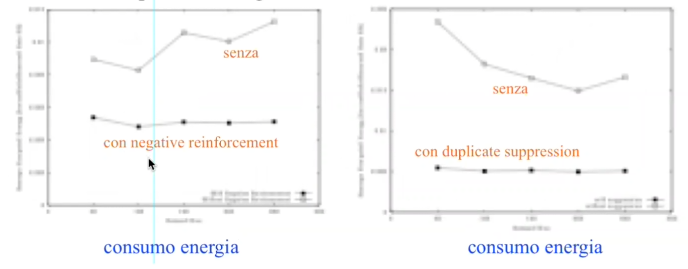
\includegraphics[width=95mm]{img/prestazion2.PNG}
\caption{prestazioni metodi di propagazione notifiche}
\label{fig:pres}
\end{figure}
\bigbreak
\noindent Figura sx: il consumo di energia senza rinforzo negativo è quasi casuale, con rinforzo negativo è più basso ma soprattutto indipendente dal numero di nodi. 
\bigbreak
\noindent Figura dx: senza soppressione dei duplicati il consumo energetico è più alto, togliendo i duplicati diventiamo indipendenti dal numero di nodi (il sistema è scalabile). 
\bigbreak
\noindent \textbf{Riassunto} \\
Direction Diffusion rientra nella categoria degli algoritmi basati sul paradigma di Reverse Path Forwarding, costruisce un cammino dai sink ai sensori e le notifiche seguono questi cammini. \textbf{Il problema di questo approccio è che non viene tollerata la mobilità dei sink, per l'approccio reverse path}. 


\section{Cost-field}
\label{sec:cf}
Concetti generali:
\begin{itemize}
    \item non vengono creati loop, considero cammini più corti. Considerando il costo fino a qualcosa, se prendessi un loop la distanza sarebbe infinita.
    \item Rumor routing supporta la mobilità del sink
    \item servizio di push (affine a mail)
    \item mantiene un'informazione di gradiente per arrivare al punto, i vicini ci dicono la distanza e la direzione dell'evento e del sink
\end{itemize}

Sono algoritmi basati su informazioni di costo per arrivare a qualche cosa: in Gradient Routing e Gradient Broadcast i nodi sanno chi è il sink e quanto costa arrivare ad esso, mentre Rumor Routing indica la distanza dall'evento. Lo stato mantenuto ai nodi è uno scalare che denota la distanza e non vengono creati loop, questo perché si costruiscono i cammini più corti (se mi accorgo della presenza di un loop, taglio il percorso in modo da renderlo più breve). Rumor Routing supportata la mobilità del sink tra una query e l'altra. 
\bigbreak
\subsection{Rumor Routing}
\noindent \textbf{Come funziona Rumor Routing?} \\
Il tentativo di un progettista di WSN, tenendo conto di star impiegando oggetti fragili e con poca energia, è cercare di ottimizzare il bilanciamento tra gli aggiornamenti e le query. Le query sono generate dalle entità interessate all'accadere di un evento in una zona dove la WSN è piazzata, gli aggiornamenti sono le risposte date dai sensori in loco in risposta alle query. Ciò dipende fortemente dall'applicativo, il primo esempio riguarda sensori che ogni mezzora riportano il dato di temperatura contro sensori che rilevano la presenza di fumo per monitoraggio degli incendi, nel primo caso ho eventi periodici - nel secondo caso potrebbe essere che per settimane, mesi o anni il sensore non si attivi mai. 
\begin{itemize}
    \item Data Flooding - pochi eventi ma tante query: è il caso del monitoraggio degli incendi (i guardia parchi dopo un'estate torrida monitorano spesso la presenza di eventi che portano ad incendi, ma gli eventi di per sé potrebbero essere pochi)
    \item Query Flooding - tanti eventi ma poche query: periodicamente un evento è mandato ai sink, i sink potrebbero anche non generare una query. 
\end{itemize}
In generale se dobbiamo fare flooding di qualcosa, scegliamo di fare flooding di ciò che è meno. Nel primo caso scegliamo di fare un flooding di eventi (costa meno perché gli eventi sono sporadici) e in questo modo portiamo l'evento in tutta la rete, magari qualche nodo è interessato. Nel secondo caso vale il contrario: viene fatto flooding delle query, i sink chiedono sporadicamente ma quando questo succede c'è alta probabilità di trovare almeno una notifica dell'evento che si sta verificando (porto le query per tutta la rete, probabilmente vicino a dove l'evento si sta verificando). 
\bigbreak
Rumor Routing cerca di bilanciare query/eventi senza sapere quanti saranno. In RR i sensori funzionano sempre (in DD i sensori non facevano nulla fino a che non ricevevano un interest), hanno codice a bordo che gli dice che cosa osservare e quando notificare (o in alternativa hanno dell'intelligenza a bordo), non è necessario che gli arrivi un interest che comunichi a che evento e ogni quanto interessarsi. 
\bigbreak
Con tecniche di diffusione random Rumor Routing distribuisce sia query che notifiche, senza però sprecare risorse. In RR il concetto di notifica non è una descrizione completa di un evento, è una traccia (briciola di pollicino) che ci dice "se vuoi avere informazioni sul movimento di quadrupedi, devi andare in quella specifica direzione". La diffusione casuale di queste notifiche è una diffusione di messaggi molto piccoli (che cosa, in che direzione, a che distanza). 
\bigbreak 
Diffusione casuale, ci sono due estremi:
\begin{itemize}
    \item Uni-cast: i due estremi sono due nodi. Il messaggio, che sia query o traccia, percorre un cammino casuale all'interno del grafo che è sempre uni-cast. Esiste una sola copia del messaggio.
    \item Flooding: non viene scelta una strada da far percorrere ai miei dati, le scelgo tutte. Genero tante copie di messaggio a seconda di a quanti vicini voglio mandarlo
\end{itemize}
Come progettisti dobbiamo decidere come muovere la diffusione casuale all'interno di questi estremi. Questo ci permette di trovare il compromesso query/notifiche. \\ L'obiettivo è che i nodi mantengano delle rotte all'evento, comprensive di costo. I nodi devono essere capaci di mantenere una lista di vicini, in RR vogliamo sapere prima chi sono i vicini. La mia strategia randomica risparmia, non arrivando a fare flooding, scegliendo un sottoinsieme di vicini al quale inoltrare le notifiche - anche se usa un canale wireless intrinsecamente broadcast - l'indirizzamento non è broadcast. Se scelgo un sottoinsieme metto nel messaggio l'indirizzo dei vicini a cui lo sto mandando, non sono loro a palesarsi, è il nodo mittente che deve conoscere i suoi vicini (ad esempio è possibile usare il beaconing: piccolo messaggio che un dispositivo manda per farsi conoscere, contenente il proprio indirizzo). 
\bigbreak
Teoricamente la diffusione di query e notifiche dovrebbero scontrarsi: nel momento in cui viene mandata la query, con alta probabilità, dovrebbe inciampare in una notifica di evento, potendo seguire quella traccia. Se RR non da una risposta, c'è un paracadute di sicurezza: uso Direct Diffusion. Se ho un forte sospetto che l'evento si stia verificando ma non ricevo nulla dai sensori tramite RR, faccio flooding una volta con DD. 
\bigbreak
\noindent \textbf{Idea generale} 
\begin{figure}[h]
\centering
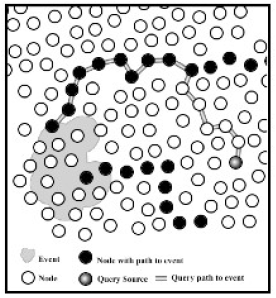
\includegraphics[width=50mm]{img/rumor.PNG}
\caption{idea generale di RR}
\label{fig:rr}
\end{figure}
\bigbreak
La macchia grigia corrisponde all'area dove l'evento si sta verificando. I puntini bianchi sono sensori, i punti bianchi dentro la chiazza grigia sono sensori già programmati per osservare il verificarsi di uno specifico evento, per questo sono in grado di mandare notifiche riguardanti quell'evento (non vuol dire che le mandano necessariamente, componente randomica). \\ Nella chiazza grigia ci sono due nodi - uno in alto e uno interno in basso, in nero - che hanno osservato l'evento e hanno tirato una moneta (con moneta è al 50\%, in realtà decide il progettista), se il risultato del lancio è positivo avviene la creazione di una notifica. Gli altri nodi interni bianchi hanno lanciato una moneta e conseguentemente a ciò che è uscito, non hanno propagato la notifica. La componente randomica è nel nodo che decide se generare una notifica o meno. 
\bigbreak
\noindent Il nodo che genera una notifica sceglie casualmente solo uno dei suoi vicini al quale inoltrarla (viene mandato un messaggio del tipo "a un hop da me si è verificato l'evento", il ricevente memorizza quindi che quella è la strada per arrivare all'evento e che si trova a due hop da esso), il nodo ricevente fa la stessa cosa scegliendo a caso un suo vicino e via così. 
\bigbreak
\noindent Il nodo grigio sferico genera una query: sceglie un vicino casuale, gli manda una copia della query, il nodo bianco che ha ricevuto la query non ha risposte ma sa di essere a un hop dal nodo che ha generato la richiesta, esso genera a sua volta una scelta casuale tra i suoi vicini e manda una copia della query. I restanti nodi bianchi ricevono la query registrando la loro distanza dal nodo grigio che l'ha generata ma nessuno ha una risposta, scelgono ciascuno un proprio vicino fino a trovare un nodo nero. Il nodo è nero in quanto è stato attraversato dalla traccia. 
\bigbreak
\noindent La query è inciampata in una traccia, la query inizia a viaggiare deterministicamente (il nodo nero sa di essere a 9-hop dall'evento e conosce chi è il nodo dal quale gli è arrivata la notifica) seguendo il reverse path verso l'evento. Il nodo nero interno alla chiazza grigia, riceve la query, genera la descrizione completa dell'evento e la fa viaggiare indietro fino alla sorgente della query. 
\begin{figure}[h]
\centering
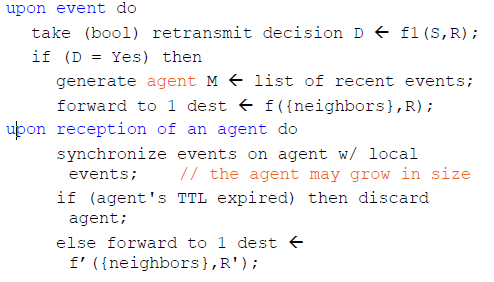
\includegraphics[width=100mm]{img/pse.PNG}
\caption{pseudo-codice}
\label{fig:ps}
\end{figure}
\bigbreak
La parte superiore è relativa a un sensore che sta nella chiazza grigia e quindi osserva l'evento (upon event). Quando vede l'evento prende una decisione di ritrasmissione booleana (l'outcome è 0 o 1), questo è il risultato di una funzione $f1(S,R)$ dove R è parametro casuale ed S è stato del nodo. Se la risposta è si, il nodo genera un agente con payload una lista di eventi osservati di recente (il nodo si è svegliato perché ha visto l'evento, ma posso riempire con eventi recenti). Il nodo inoltra a una sola destinazione utilizzando una funzione $f(\{neigh\}, R)$ con R componente casuale e {neigh} insieme di vicini (i vicini cambiano nel tempo, pesco da quelli attivi). 
\bigbreak
La parte inferiore riguarda i nodi che ricevono una notifica ma non hanno osservato l'evento. Questi nodi sincronizzano gli eventi sull'agente con gli eventi locali (in figura in basso, l'agente grigio chiaro incontra la traccia color scuro. L'agente grigio viene caricato anche con l'evento grigio scuro). \\ Tutti gli eventi che il nodo non conosce vengono memorizzati dal nodo, da chi proviene e la distanza. Oltre a questo, se nell'agente ricevuto c'è ancora spazio nel payload e il nodo che ha ricevuto l'agente conosce/vede degli eventi non notificati nell'agente, può caricarli sull'agente. L'agente può crescere in taglia perché si carica di altre notifiche. 
\bigbreak
Dopo di che se il TTL dell'agente è scaduto, ha fatto tutti gli hop che poteva fare, scarto l'agente. Se ci sono ancora hop fattibili, l'agente è inoltrato a una sola destinazione tramite una funzione $f'(\{neigh\}, R)$. 
\bigbreak
Le funzioni di scelte casuali possono essere diverse per ogni nodo, vengono scelte dal progettista come le variabili randomiche R. Le variabili randomiche R potrebbero esserlo non del tutto: ad ex. posso scegliere una sorta di peso di probabilità in base a quanto bene sento i miei vicini, oppure - in una rete non omogenea, 3tier - assegno peso maggiore a nodi più potenti. 
\begin{figure}[h]
\centering
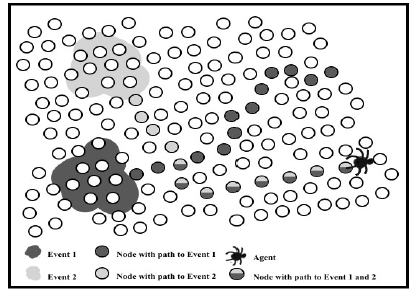
\includegraphics[width=80mm]{img/agent.PNG}
\caption{pseudo-codice}
\label{fig:ps}
\end{figure}

\bigbreak
Se la query non intercetta mai la notifica? L'analisi ci dice che la probabilità di intersezione query/traccia non è bassa. \\ Ci sono due tipi di percorsi casuali in una rete:
\begin{itemize}
    \item random walk: il movimento casuale è generato scegliendo la direzione di movimento, la velocità e la distanza o il tempo da percorre. Così raggiungo la mia nuova posizione, quando arrivo genero una nuova direzione, velocità e tempo/distanza e così via. Se la direzione e il tempo mi fanno raggiungere un bordo dell'area che sto considerando, o l'oggetto torna indietro oppure esce - con angolo speculare - dal bordo opposto. Se scelgo questa politica per gli agenti, l'agente si raggomitolerà in una zona e si sposterà poco, sprecando il proprio TTL.
    \item random waypoint: scelgo un punto di arrivo esistente (uno dei pallini bianchi) e mi muovo verso quella direzione. Quando arriva in quel punto, può avere un punto di off e sostare un po', dopo di che sceglie un altro punto esistente verso il quale dirigersi. Non ha il problema dei bordi e distribuisce meglio all'interno dello spazio. Le tracce lasciate dal RWaypoint sono molto diverse dal RWalk, si distribuisce molto più uniformemente sull'area. 
\end{itemize}
In entrambi i casi è possibile formalizzare con leggi statistiche, la probabilità di intersezione non è bassa. 
\bigbreak
\noindent \textbf{Loop e cammini} \\
Non è consentita la presenza di loop, infatti ogni nodo esprime la distanza dall'evento, in Rumor Routing, se ci fossero loop questa distanza diventerebbe massima, cioè infinita. 
\begin{figure}[h]
     \centering
     \begin{subfigure}[b]{0.3\textwidth}
         \centering
         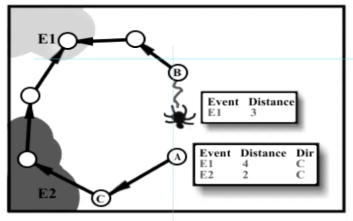
\includegraphics[width=50mm]{img/prima.PNG}
         \caption{Step 1}
     \end{subfigure}
     \hfill
     \begin{subfigure}[b]{0.3\textwidth}
         \centering
          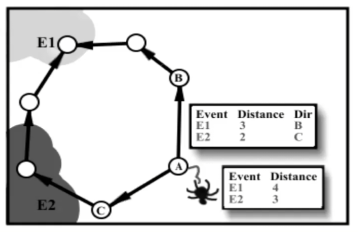
\includegraphics[width=50mm]{img/prima2.PNG}
          \caption{Step 2}
     \end{subfigure}
    \caption{Cammini }
    \label{fig:camm}
\end{figure}
\bigbreak
Figura sx: il nodo A che non sta osservando un evento, ha delle informazioni (raggiunge evento E2 in due hop passando per il nodo C) e nel passato ha incontrato un agente che gli ha detto che può raggiungere l'evento E1 che sta a distanza 4-hop passando per il nodo C. 
Il nodo nell'evento E1 si sveglia e vede che l'evento si sta ancora verificando, lancia la moneta e - nel caso - genera un agente e lo manda al nodo alla sua destra. L'agente è inoltrato fino al nodo B, questo memorizza l'informazione per raggiungere l'evento E1 e la distanza e manda avanti l'agente verso il nodo A (l'agente contiene l'informazione sull'evento E1 a distanza 3).  
Quando il nodo A riceve l'agente generato da B deve sincronizzarsi: l'agente non porta informazioni riguardo all'evento E2 che invece A conosce. Il nodo A carica sull'agente le informazioni sull'evento E2.
\bigbreak
Figura dx: il payload dell'agente contiene informazioni sia sull'evento E1 che sull'evento E2, per la sincronizzazione. Inoltre, quando A riceve l'agente generato da B, sa già come raggiungere l'evento E1. Tuttavia la distanza che aveva il nodo A era di 4-hop, mentre l'agente gli sta comunicando che c'è un cammino diverso a distanza 3-hop. Il nodo A si aggiorna. \\ Il vecchio cammino non è eliminato, sarebbe problematico dire a tutti i nodi di cancellarlo, inoltre è comodo perché permette, ad ex. al nodo C se mai riceverà una query per l'evento E1, di avere indicazioni per arrivare all'evento. 
\bigbreak
\noindent \textbf{Query processing} \\
\begin{figure}[h]
\centering
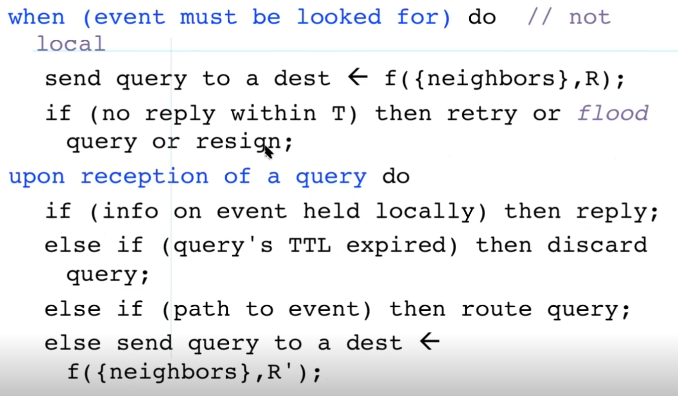
\includegraphics[width=90mm]{img/qyeru.PNG}
\caption{Esecuzione query}
\label{fig:eq}
\end{figure}
\bigbreak
Quando un nodo cerca un evento (\textit{event must be looked for}), prima di tutto guarda se localmente sa come raggiungerlo. Se non ha questa informazione, sceglie uno tra i suoi vicini attivi con una politica di scelta casuale, e gli manda la query. Questo nodo aspetta per un tempo T, se non riceve una risposta può generare un'altra query scegliendo un nodo diverso al quale inoltrarla oppure fa flooding della query (la prima soluzione la si usa quando si ritiene che l'evento non si stia verificando oppure si hanno vincoli meno stringenti, ex: devo vedere un quadrupede non importa se non ne vedo qualcuno. La seconda soluzione la si usa quando si ha una forte esigenza di essere notificati della presenza dell'evento oppure se si ha una forte evidenza che questa cosa si stia verificando, allora si può fare flooding. La terza soluzione è rinunciare). \\ La seconda parte riguarda un nodo che riceve una query generata da qualcun' altro (\textit{upon reception of a query}). Il nodo può aver osservato direttamente l'evento (\textit{info on event held locally}) e genera una notifica con la descrizione completa dell'evento. Se il nodo invece vede che il TTL (Time To Live) della query è scaduto, la query viene scartata. Se il nodo ha informazioni sul cammino per l'evento (\textit{path to event} instrada deterministicamente la query lungo quel cammino. Se non è nessuno di questi casi, allora il nodo manda la query a un destinatario scelto, con politica casuale, tra i suoi vicini attivi in quel momento. 
\bigbreak
In generale, quindi stiamo facendo vagare la query e gli agenti a caso nello spazio, siamo felici e fortunati se le due inciampano tra loro, vogliamo quindi che ci sia una probabilità alta di intersezione. Per fare questo usare la tecnica Random Walk non è il massimo: la query e l'agente si raggomitolano dove partono senza fare grandi salti che consentano di espandersi ampiamente per la rete, devo scegliere saggiamente la legge statistica. Usare Random Waypoint porta a risultati migliori.
\bigbreak
\noindent \textbf{Rumor: discussione e ottimizzazione sull'aumentare probabilità di incontro tra query/agenti} 
\begin{itemize}
    \item vogliamo massimizzare la probabilità di intersezione tra agenti e query. Per far questo potrei far muovere in linea retta query e agenti: un sensore che genera un agente lo manda in direzione sud o nord e un nodo che genera una query la manda in direzione est o ovest. I cammini sono ortogonali, prima o poi si forma una "griglia" e si incontrano query e agenti. Come faccio?
    \begin{itemize}
        \item[-] Antenna uni-direzionale e bussola, la bussola mi dice dove sta il nord e l'antenna mi permette di sparare il segnale in quella direzione
        \item[-] Aggiungo nella rete la capacità di conoscere la posizione di nodi. Il nodo necessita un algoritmo di localizzazione a bordo, inoltre è necessario,quando i nodi mandano i loro beacon per farsi conoscere, che aggiungano anche la propria posizione. 
        \item[-] Posso provare ad approssimare una linea retta: un messaggio (agente/query) viaggiando, carica una lista dei nodi visitati. Quando un nodo riceve uno di questi messaggi e deve re-inoltrarlo, sceglie un suo vicino che non compare nella lista (visito un nodo nuovo e sposta il messaggio più lontano e rompe anche i loop). Posso fare qualcosa di più drastico, non solo ricordo la propria lista dei vicini, ricorda la lista dei vicini dei vicini. Dove salvo questa informazione? lo metto nel payload dell'agente, ma questo mi serviva per caricarci tutti gli agenti che poteva imparare in più dai nodi che visita. Come mi gioco lo spazio nel payload dell'agente?
    \end{itemize}
    \item Configuro i nodi della rete in modalità promiscua, sono spenti e si accendono quando ricevono un frame indipendentemente dall'indirizzo a cui sono destinati. La sorgente dell'agente manda l'agente in uni-cast a un nodo, ma questo viene sentito e registrato in cache da tutti i nodi vicini della sorgente e così via. Creo delle "strade più larghe", quando viene beccato un nodo al limite di questa strada, quello reindirizza il cammino al centro della strada. 
    \item I costi dipendono dal numero di query ed eventi. Dobbiamo moltiplicare il TTL per il numero di query/agenti.
    \item Gli agenti dovrebbero avere un TTL grande (tanti hop a disposizione) in modo da avere il tempo di viaggiare e spostarsi sensibilmente nella rete, visitando tanti nodi.\textbf{Il decremento del TTL quando l'agente trova la traccia viene sospeso}.
    \item Gli agenti potrebbero essere ritrasmessi per evitare collisioni, per aggiungere affidabilità. 
    \item Se ci sono pochi eventi ma tante query conviene fare flooding degli eventi e viceversa. RR usa un approccio intermedio, non facendo flooding di nessuno dei due: RR può decidere tra inoltrare in unicast o inoltrare a un sottoinsieme di nodi (che possono essere tutti).
\end{itemize}
\bigbreak
\noindent \textbf{Tuning dei parametri e prestazioni} \\
Devo cercare la combinazione di parametri che mi restituisce risultati migliori. Vengono usati dei SW simulatori di reti, specificando la topologia di rete, algoritmi e protocolli che sono in esecuzione su ogni nodo. Il simulatore  genera del traffico facendolo girare nella rete fittizia, misurando le prestazioni.
\begin{figure}[h]
\centering
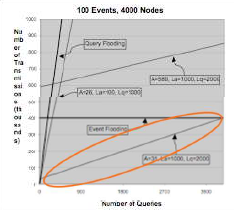
\includegraphics[width=70mm]{img/presta.PNG}
\caption{prestazioni e parametri}
\label{fig:prestazioni}
\end{figure}
 Ad ex: rete unplanned simulata con 4000 nodi, vengono generati 100 eventi - vediamo che parametri mi ridanno le prestazioni migliori in risparmio energetico. Per gestire 100 eventi e permettere ai sink di trovarli, se facciamo query flooding (Directed Diffusion) molto presto, cioè al crescere di numero di query per raggiungere gli eventi, il numero di trasmissioni diventa molto alto. Facendo event flooding, intesto come descrizione completa dell'evento, quando un nodo genera una query trova il risultato localmente, per cui il numero di trasmissioni è indipendente dal numero di query generate. \\ Le rette inclinate hanno associate tre etichette, la prima indica il numero di agenti che vengono generati da ogni sensore che sta osservando l'evento come attivo, la seconda indica il TTL degli agenti e la terza indica il TTL delle query. \\ La retta evidenziata in arancio è ottima perché permette di utilizzare RR risparmiando in prestazioni rispetto a tutte e due le politiche di flooding. Sui sensori reali mettere del codice eseguibile con i parametri trovati, 31 agenti, TTL agenti = 1000, TTL query = 2000 hop. 

\section{Ma non solo}
\label{sec:solo}
\begin{itemize}
    \item Ci sono anche approcci gerarchici: più semplice, perché assumo di poter dare più lavoro a nodi con più risorse, computazione, memoria, antenna, batterie.
    \item Ci sono anche algoritmi che danno garanzie real-time, nell'industria 4.0 questo è essenziale.
    \item Oppure ci sono algoritmi che sfruttano la localizzazione, ad ex: abbiamo già usato la posizione per direzionare il flooding di DD verso un'area target. Oppure far viaggiare agenti/query in linea retta conoscendo le coordinate dei vicini in RR.  
\end{itemize} 

\chapter{PSFQ (Pump Slowly, Fetch Quickly)}
\label{cap:ptaw}
Bibliografia - si trovano in lezione e materiali didattici: 
\begin{itemize}
    \item[-] Chieh-Yih Wan, Andrew T. Campbell, Lakshman Krishnamurthy, \textit{Pump-Slowly, Fetch-Quickly (PSFQ): A Reliable Transport Protocol for Sensor Networks}
\end{itemize}
\bigbreak
Ci potrebbero essere vincoli molto stringenti sia in latenza che in affidabilità, ad esempio vale per l'industria 4.0: ci sono device, controllori che prendono i dati dal sink e li analizzano, a questo punto possono mandare direttive ai sensori o agli attuatori cambiandone il codice o i parametri per fare in modo che operino in modo diverso. Vorrei che una notifica di questo tipo - in un impianto industriale - avesse una possibilità del 99.9\% di arrivare a destinazione. Vorrei un protocollo affidabile dall'EDGE ai sensori, se perdo la notifica mandata da un sensore, oltre che essere probabilmente meno grave, ci saranno tanti altri sensori nell'area che mi mandano una notifica simile. Se perdo la query del sink, tutti i sensori in area non sanno di dover monitorare l'evento. 
\bigbreak
In reti wired il protocollo affidabile è TCP, esso aspetta degli ACK o degli NACK. Se questi non sono ricevuti, allo scadere del timeout TCP richiede la ritrasmissione del dato. L'affidabilità di TCP andrebbe benissimo per il contesto industriale, quello che non funziona è la latenza (devo richiedere e aspettare la ritrasmissione di messaggi, se voglio ottenere affidabilità devo perdere tempo a fare qualcosa. In alternativa non setto nemmeno la comunicazione e uso UDP, perdendo in affidabilità). Inoltre TCP è usato da due solo entità che comunicano, in una WSN ho molti sensori, molti attuatori e possono essere molte anche le sorgenti. Se dovessimo usare TCP, la sorgente dovrebbe raccogliere molteplici ACK dalle varie destinazioni. La sorgente manda in broadcast i dati, indirizzamento broadcast, mettiamo che riceva solo un sottoinsieme di ACK dalle destinazioni. Come mi comporto? Ritrasmetto solo a chi non mi ha risposto? Ritrasmetto a tutti? \\ E' difficile perché non c'è conoscenza delle destinazioni, non so chi siano e non so quante siano. Inoltre mi baso sullo scadere del timeout con cui attendo l'ACK, ma potrebbero esserci nodi destinazione in zone periferiche della rete oppure altri molto vicini al sink, ho problemi nel setting del timeout. \\ Crying baby: un algoritmo con questa caratteristica aspetta il bambino che si lamenta maggiormente - il device con meno banda, batteria e memoria - che rallenta tutto il sistema. \\ Un altro problema è il Bit Error Rate su canale wireless, le politiche di TCP di ritrasmissione non sono adeguate perché tendono a rallentare per non congestionare la rete. Ma in un canale wireless dovrebbe diventare più aggressivo per ovviare a interferenze e collisioni. 

\begin{figure}[h]
\centering
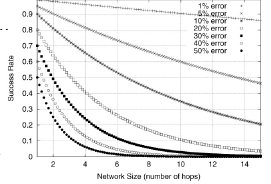
\includegraphics[width=90mm]{img/grafico.PNG}
\caption{Influenza tasso di errore}
\label{fig:gre}
\end{figure}
Sulle ascisse c'è la misura del diametro della rete, numero di hop necessari per andare tra i due nodi più lontani. Sulle ordinate vediamo l'affidabilità di portare un messaggio. Il grafico è fatto assumendo che non ci siano politiche di ritrasmissione. Le diverse curve ci dicono che abbiamo una probabilità di errore tra due apparati, che sono nello stesso raggio radio, di mandarsi un messaggio uguale a \textit{p}. \\ Suppongo che la destinazione sia a \textit{n} hop dalla sorgente, dobbiamo fare successo(1hop) and successo (2hop) and ... and successo (nhop), ottenendo che la probabilità che il messaggio arrivi è $(1-p)^n$. 
\bigbreak
La probabilità, andando avanti di hop in hop, diventa sempre più piccola. L'idea per risolvere il problema è di garantire affidabilità non sull'intero percorso, non lasciando tutto il lavoro a sorgente e destinazione, ma su ciascun hop. Questo permette anche di correggere il problema appena si presenta e non quando arriva a destinazione. \\ Se abbiamo migliaia di nodi è un problema la trasmissione di ACK: dobbiamo mettere in preventivo di far gestire al sink migliaia e migliaia di ACK, aumentando il rischio di collisioni e interferenze. \\ Sarebbe meglio operare con dei NACK e intervenire subito quando si presenta il problema.
\bigbreak
PSFQ nasce dall'analisi critica di TCP e dai suoi limiti sulle WSN. Questo algoritmo inietta lentamente i dati nella rete ma cerca di recuperarli molto velocemente quando vede un problema. 
\bigbreak
\noindent Obbiettivi:
\begin{itemize}
    \item Affidabilità nella consegna dei dati: non può essere del 100\% a causa della fragilità della rete. Potremmo ritrasmettere il messaggio un certo numero di tentativi, dopo di che sospendo. Il sensore destinazione sa che non ha ricevuto qualcosa e si auto-spegne, fino all'arrivo della configurazione successiva. 
    \item Minimo supporto dall'infrastruttura sottostante: si richiede che la rete sappia fare broadcast one-hop e che ci sia un algoritmo di routing, RR o DF o derivati, a livello 3.
    \item Minimo scambio di messaggi di controllo per affidabilità: uso le energie del sistema per scambiare i dati e non per informazioni di controllo.
    \item Correttezza anche con qualità canale molto bassa
    \item Latenza ridotta: se stiamo ri-configurando sensori o attuatori vorrei che avvenisse nel giro di secondi, non giorni (in più ci sono sensori lontani e vicini, vorrei che commutassero tutti insieme)
\end{itemize}

\noindent \textbf{User node} sono i nodi che generano dati che devono essere mandati e ci sensori destinatari che li ricevono. 
\bigbreak
\noindent Organizzato in 3 (4) fasi:
\begin{enumerate}
    \item \textbf{PUMP}: iniezione dei dati, direttive o riconfigurazioni, nella rete. Lo user node invia lentamente i dati con associato un numero di sequenza. Lo user node li manda in modo che il tempo che intercorre tra un messaggio inviato e il successivo, permetta - ai nodi della rete - di recuperare il dato perso se si è verificato un errore. Questo mi permette di non riempire il buffer del nodo con messaggi in attesa di ACK, questo ad un certo punto potrebbe portare alla perdita di messaggi. Permetto al nodo di avere del tempo di processare i dati e svuotare il buffer. 
    \item Il nodo che riceve messaggio $m-1$ e poi $m+1$, capisce che gli manca un messaggio e passa alla fase di fetch
    \item \textbf{FETCH}: cerca di recuperare il messaggio che si aspettava. Questo viene fatto usando i NACK, non vengono mandati fino alla sorgente (magari il problema è vicino al nodo, è uno spreco di energia ritornare fino alla sorgente), li mando ai vicini, tentando di sopprimere i duplicati che mi arrivano dai vicini
    \item \textbf{REPORT}: se abbiamo bisogno di passare da un approccio con NACK a un approccio con ACK (facoltativo)
\end{enumerate}

\section{PUMP}
\label{sec:pUMP}
Supponiamo che lo user node abbia un insieme di dati da mandare (ex. nuovo codice eseguibile completo da mandare ai nodi - non possiamo mandarlo tutti insieme, lo spezziamo in più messaggi), manda il dato in broadcast ai suoi vicini ogni \textit{T\_min}. I nodi intermedi mantengono cache dei messaggi ricevuti, il numero di sequenza mi permette di scartare messaggi che il nodo ha già in cache oppure di capire se il dato è nuovo. A questo punto il nodo elabora localmente il dato e lo distribuisce broadcast dopo un tempo casuale nell'intervallo \textit{[T\_min, T\_max]}. I nodi intermedi potrebbero essere più lenti della sorgente.  
\begin{itemize}
    \item T\_min per il controllo di flusso: la sorgente più veloce di così non va e anche i nodi intermedi non re-inoltrano prima di questo tempo. 
    \item T\_max per de-sincronizzazione: entro quanto tempo devo recuperare. Siamo in una rete unplanned densa, se ho una collisione i dati si perdono: la de-sincronizzazione consiste nel far ricevere ai nodi un dato dallo user node e di non ri-trasmetterlo subito. Teniamo conto che lo user node ha mandato il dato in broadcast ai suoi vicini, se nodi vicini mandano i messaggi dopo lo stesso tempo, i messaggi collidono. Pescare casualmente permette di non sovrapporre i segnali dei nodi. 
\end{itemize}
Possiamo stimare un upper bound per far arrivare una sequenza di \textit{n} dati su un cammino con un certo numero di hop è
\begin{equation}
    D(n) = T_{max}*n*num_{hops}
\end{equation}

\section{FETCH}

\begin{figure}[h]
\centering
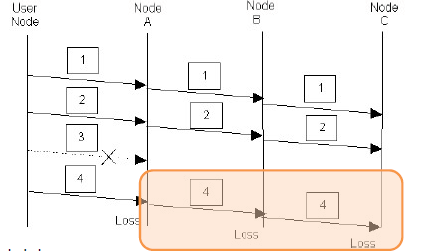
\includegraphics[width=100mm]{img/espsfq.PNG}
\caption{Idea generale}
\label{fig:gre}
\end{figure}
A sinistra c'è un nodo utente che manda i suoi messaggi a tutti i suoi vicini, il nodo vicino A riceve i messaggi, li salva in cache e li manda in broadcast ai propri vicini. Il nodo B e il nodo C fanno la stessa cosa del nodo A. \\ Il problema sta che viene perso il messaggio con numero di sequenza 3: il nodo A ha una certa tolleranza temporale nel ricevere i messaggi, ma quando riceve 4 capisce che qualcosa è andato male. Il nodo A genera un NACK e lo manda - con TTL = 1 - hop richiedendo il messaggio 3 mancante. 
\bigbreak
Il nodo A non inoltra il messaggio 4 ai suoi vicini. Supponiamo che questo avvenga (riquadro arancione in figura): i messaggi non possono essere consegnati all'applicazione sovrastante perché manca un messaggio, viene iniziata la procedura di recupero del messaggio 3. Il nodo A potrebbe iniziare a mandare il messaggio 4 al nodo B, il nodo B non ha nemmeno lui ricevuto il messaggio 3. A questo punto anche il nodo B dovrebbe entrare nella fase di FETCH, generando un NACK. 
\bigbreak
Stiamo parlando di reti WSN unplanned e dense, c'è un'alta probabilità che la trasmissione del NACK del nodo A si sovrapponga alla trasmissione del NACK del nodo B, questo crea interferenza per tutti i nodi vicini di A e B (compreso il nodo che ha il messaggio 3). Se non riceve un NACK, lo user node pensa che stia andando tutto bene. 
\bigbreak
Quello che accade è che il nodo A riceve il messaggio 4 e lo memorizza nella propria cache senza passarlo ai nodi vicini. Fa partire la fase di FETCH e solo dopo che avrà ricevuto il messaggio 3, passa il messaggio 3 e messaggio 4 alla propria applicazione, e poi manda in broadcast il messaggio 3 e 4 ai propri vicini. Nel nodo B non succede nulla, non ricevono più messaggi dopo il messaggio 2, aspettano che il messaggio gli arrivi (senza generare NACK e quindi senza interferire e senza usare energia per trasmettere). 
\bigbreak
Se un nodo ha visto un gap nella sequenza di messaggi inizia la fase di fetch. \\ $\Phi(i)$ mi dice che probabilità ho di recuperare un messaggio che mi manca alla $i-esima$ ritrasmissione (mandando $i$ volte un NACK). \\ $p$ è la probabilità di errore sul canale, quindi $1-p$ è la probabilità che io riceva un messaggio mandato da un mio vicino.
\begin{itemize}
    \item $\Phi(0) = 0$: se non genero nessun NACK, non richiedo il messaggio e non lo avrò più
    \item $\Phi(1) = (1-p)^3$: ci sono tre eventi: arrivo del messaggio successivo che mi rivela il gap in sequenza, l'invio del mio NACK e l'invio della ritrasmissione (tutti avvengano su un hop e ciascun ha $(1-p)$ di successo).
    \item $\Phi(n) = (1-p)^2 * [1-p-\Phi(1)-\Phi(2) - ... - \Phi(n-1)]$: nella parentesi quadra considero la probabilità di successo $1-p$ alla quale tolgo il fatto di non aver successo in $\Phi(1), \Phi(2) ... \Phi(n-1)$ (ad ex. può essere che il NACK è stato mandato ma nessun ha ritrasmesso il messaggio mancante)
\end{itemize}. 
Considero ora $\omega(n)$ cioè la probabilità di avere successo entro $n$ tentativi. Ce la posso fare o al primo tentativo oppure al secondo fino al tentativo n-1, $\omega(n) = \Phi(1) + \Phi(2) + ... + \Phi(n)$. 
\bigbreak
$(1-p) + (p + \Omega(n))$ mi indica la probabilità di recupero in $n$ tentativi. La parte $p*\Omega(n)$ mi dice che qualcosa va male con probabilità $p$ sui tentativi precedenti. $(1-p)$ è la probabilità che all'ennesimo colpo riesco ad ottenere il recupero.
\bigbreak
Dal grafico della slide 8, sulle ordinate ho la probabilità di successo, nelle ascisse probabilità di perdita di un pacchetto su un hop. La retta più in basso è quando non faccio ritrasmissioni, alla crescita della probabilità di perdita di un pacchetto, la probabilità di recuperarlo ricresce linearmente. Se faccio ritrasmissioni, le curve sopra la retta, la probabilità di successo si alza. Le curve più in alto sono sovrapposte. 
\bigbreak
Il numero magico è 4 (se facessi più di 4 ritrasmissioni non aggiungerei un granché al success rate). La curva con 3 ha un success rate più alto delle curve con 5 e 7, le curve con 5 e 6 sono sovrapposte. E' un compromesso tra 3 ma senza andare a 5,7 ritrasmissioni massime consentite. 

\subsection{Numero magico 4}
Il numero magico 4 viene usato in fase di PUMP: un nodo riceve un messaggio da qualche suo vicino, guarda se il messaggio è in cache, se così è lo scarta. Se il messaggio non è in cache ed è in sequenza, metto il messaggio nella cache, genero un tempo casuale tra $t_{min}$ e $t_{max}$ e quando questo tempo scade, faccio il broadcast del messaggio. Ci sono delle volte in cui questo non è vero, introduciamo il numero magico 4. Il nodo pesca un tempo casuale e non ha null'altro da fare che aspettare che questo timeout scada per rifare broadcast. In una WSN unplanned e densa, il nodo ha tanti vicini e uno di loro mi ha mandato il messaggio. Questo nodo sarà a monte, vicini all'user node, rispetto a me. Gli altri nodi vicini potrebbero aver ricevuto lo stesso messaggio. Mentre aspetto che il mio timeout scade, vedo che alcuni miei vicini mandano un messaggio che io ho ancora pending, cioè sto aspettando che scada il mio timer relativo a quel messaggio. Una volta che conto 4 vicini, sono arrivata al numero magico. Se faccio 4 volte la ritrasmissione mi basta così, so che se aggiungo ritrasmissioni non aggiungo niente di significativo al success rate, anzi occupo il canale, spreco energie e risorse. Così sopprimo il mio timer, mantengo il messaggio in cache (per rispondere ad eventuali NACK). 
\bigbreak
Come uso il numero magico 4 nella fase di fetch? 
\begin{itemize}
    \item un nodo rileva un gap nella sequenza crea un messaggio NACK che aggrega tutti i gap rilevati (il nodo manda nel NACK (3 - 5 - 6 - 9 - 11) quindi individua i messaggi mancanti 4 - 7 - 8 - 10). \textit{Abbiamo detto che non vengono passati messaggi fino a che non rispettano la sequenza, può darsi che sia proprio questo il nodo vicino allo user node che riceve frammenti}. Il NACK aggrega i gap rilevati e manda gli estremi per indicare dove ha individuato il gap: se il nodo non ha i messaggi 15, 16, 17 manda un NACK con (14, 18) indicando che gli mancano quei tre, questo metodo per indicare i messaggi mancanti mi permette di occupare meno spazio. 
    \item il nodo genera un ritardo casuale in $[0, \Delta]$ con $\Delta$ piccolo (se i nodi iniziano a mandare NACK tutti insieme creo problemi di interferenza, per questo motivo decido un ritardo casuale), dopo il quale invia il primo NACK se non ne sente altri per medesimi gap (il nodo nel frattempo ascolta e sente dei nodi vicini che mandano con successo dei NACK e questi coprono tutti i gap di cui il nodo aveva bisogno. Il nodo non manda il NACK, se i suoi nodi vicini riceveranno una risposta probabilmente anche il nodo considerato otterrà i messaggi che gli mancano. Se i NACK non coprono tutti i gap del nodo considerato, il nodo manda un NACK con solo il gap che non è coperto da altri nodi vicini). 
    \item il NACK può non ottenere risposta, per interferenze, collisioni o nessun ha la risposta. Se il nodo dopo il primo NACK non riceve una risposta che soddisfa i suoi gap entro un tempo $T_r$, rimanda il NACK. Il tempo di recovery è molto più grande di $\Delta$ ma più piccolo di $T_{max}$. E' minore di $T_{max}$ perché vorrei completare la procedura di recupero prima che venga mandato un nuovo messaggio (il nodo a monte deve memorizzare tutti i messaggi dopo quello mancante, ma le code dei nodi sono limitate). Re-invio il NACK al massimo 4 volte, se non ottengo quello che necessito, continuare ha poco senso perché non aumento di molto il success rate. 
    \item un nodo che riceve un NACK e possiede uno o più messaggi nei gap segnalati (non è necessario che risponda a tutti i gap) si predispone a mandare i messaggi ai nodi che li hanno richiesti. Il nodo genera un tempo casuale in $[1/4T_r, 1/2 T_r]$, allo scadere di questo timer manda la propria risposta. La risposta non è mandata unicast a chi ha generato il NACK - potrebbe succedere che ad altri nodi mancano quei messaggi ma hanno fatto soppressione di duplicati e quindi non ha mandato il NACK - la risposta è mandata broadcast one-hop. Nel caso il nodo sente reply di altri nodi che coprono gli stessi messaggi o un sottoinsieme, il nodo non rimanda tutti i messaggi ma solo quelli a cui nessun nodo ha ancora risposto. 
\end{itemize}

NACK, casi particolari:
\begin{itemize}
    \item Miglioro efficacia: mando i NACK broadcast one-hop, può darsi che ci siano vicini due-hop che sono in grado di recuperare i messaggi. L'ultima volta che re-inoltro il NACK, metto una soglia a due-hop. 
    \item Miglioro efficienza (pago costi più bassi): posso misurare la qualità del segnale con la quale ricevo dai miei vicini, quando devo chiedere qualcosa posso generare un NACK solo quando ho un gap generato in trasmissione con genitore preferito. Se ricevo trasmissioni a pezzi da un nodo dal quale storicamente ricevo male, non mi preoccupo, non mando NACK e aspetto di ricevere da nodi più "affidabili". 
    \item Miglioro efficienza: il NACK è mandato in broadcast ma nel payload dichiaro di preferire il genitore preferito, i nodi che ricevono il NACK ma non sono il genitore preferito posso raddoppiare il tempo di risposta. Questo cerca di evitare collisioni in trasmissioni con la risposta del genitore preferito.
\end{itemize}

\begin{figure}[h]
\centering
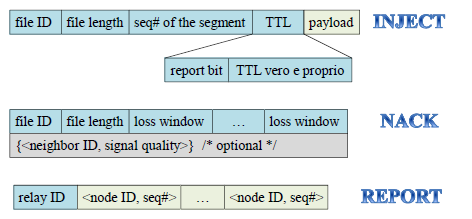
\includegraphics[width=80mm]{img/formato.PNG}
\caption{formato dei messaggi}
\label{fig:form}
\end{figure}
\noindent Fase di REPORT: fase opzionale di PSFQ. Serve se lo user node decide di passare da un approccio con ACK negativo ad uno con ACK positivi. Il coordinatore, lo user node, vuole sapere che messaggi hanno ricevuto gli altri nodi. Il problema è che avevamo scartato una soluzione TPC-like perché può portare a saturazione del canale.
\newpage
\noindent INJECT: messaggio mandato dal coordinatore nella rete, questo è poi ridiffuso da tutti i nodi nel loro vicinato. \\ Contiene:
\begin{itemize}
    \item file ID: nome arbitrario 
    \item file length: permette ai nodi di controllare, alla fine, che la sequenza di messaggi sia arrivata tutta
    \item number of segment - numero di sequenza
    \item TTL: il bit più significativo di questo campo è un report bit. L'inject è fatta dallo user node, esso specifica in questo report bit se vuole usare il paradigma positive ACK rispetto al negative ACK. Il resto è TTL vero e proprio, questo valore è deciso dallo user node. 
    \item Payload: carico di dati vero e proprio
\end{itemize}
\noindent NACK:
\begin{itemize}
    \item file ID: a che file si riferisce questo NACK
    \item file length
    \item loss window: i gap sono rappresentati da finestre che rappresentano il limite sinistro e destro del gap. 
    \item {neighbor ID, signal quality}: parametri opzionali, contengono insieme di coppie {vicino, qualità del segnale da lui ricevuto}. Mi può servire per indicare il vicino genitore preferito, oppure per fare un ranking dei miei vicini one-hop: chi è in alto in classifica pesca timer più bassi per mandarmi la risposta. 
\end{itemize}
In generale file length ci permette di affrontare il problema del last ACK. Il controllore sta mandando messaggi agli attuatori, un nodo destinatario riceve un messaggio con numero di sequenza $k$ e poi più niente. Se non indico la file length, il nodo potrebbe pensare che sia finita la trasmissione. Introdurre il campo file length in messaggi di tipo INJECT permette ad un nodo di capire se gli manca qualcosa.

\section{REPORT}
Un nodo che ha ricevuto un REPORT risponde in un tempo casuale $[0, \Delta]$ (se i report stanno viaggiando dalle foglie alla radice del grafo rischio che collidono, ho bisogno di tempi casuali), indirizzandolo al proprio genitore. Ogni nodo intermedio aggiunge la propria coppia < ID, $s_{last}$ > e reindirizza al proprio genitore. 
\bigbreak
\noindent Il tempo $T_{report}$ dev'essere due volte la distanza, in numero di hop, dal nodo che sta entrando in report mode fino al nodo più lontano da questo nel lato opposto allo user node (devo dare tempo al messaggio di INJECT fino al nodo foglia più lontano e consentire al REPORT lì creato di risalire). 
\bigbreak
\noindent Cosa succede se un REPORT si riempie? Genero un nuovo record in cui mettere le mie informazioni aggiuntive. Inoltro prima il mio nuovo REPORT e poi quello pieno (se lasciassi andare prima quello pieno, anche il nodo upstream vede un report pieno e genera un altro nuovo REPORT). 

\section{Problemi vari in PSFQ}
\begin{itemize}
    \item Problema uno: un nodo perde gli ultimi segmenti fino alla fine del file, non può sapere se ci sono gap perché non gli arriva più nulla, non sa se il problema è sopra di lui o è un problema suo. Osservando file length si rende conto che qualcosa gli manca. PSFQ prevede che un nodo che non ha ricevuto tutto possa eseguire un \textbf{recupero proattivo}. Ogni volta che un nodo riceve un messaggio fa partire un timer $T_{pro}$, alla scadenza del quale manda un NACK. 
    \begin{equation}
        T_pro = min{\alpha (S_max - S_last) T_max, \alpha n T_max} 
    \end{equation}
    $\alpha$ è una misura di affidabilità del canale, lo scelgo tanto più alto quanto il canale non è affidabile, questo perché mi preoccupo meno se il canale è inaffidabile e aspetto meno tempo. Se il canale è più affidabile, probabilmente c'è un problema davvero. \\ $S_{max}$ numero di sequenza che dovrebbe avere l'ultimo messaggio (lo calcolo dividendo file length/dimensione payload). \\$S_{last}$ ultimo segmento ricevuto. Se ho ricevuto pochi segmenti $S_{max} - S_{last}$ è molto grande, rendendo grande anche $T_{pro}$, prima di agitarmi mi concedo di aspettare un po' più di tempo e vedere come si evolve la situazione. Se ho ricevuto quasi tutti i segmenti, mi allarmo prima e adotto una comportamento proattivo prima. \\ $\alpha n T_{max}$ dove $n$ è numero massimo di messaggi immagazzinabili in cache (so quanti messaggi possono memorizzare i nodi, se inizio a recuperare quando le cache sono in overflow, alcuni messaggi andranno persi). \\ Tra i due vince il minore, l'esigenza più forte (ho più esigenza di recuperare prima che qualche buffer sia pieno? Oppure i buffer sono molti grandi e a me interessa recuperare agilmente upstream?). 
    
    \item Tutti i dati stanno in un segmento solo, il coordinatore manda un INJECT, ma qualche nodo non riceve proprio questo messaggio. E' una situazione scomoda, alcune destinazioni non conoscono nemmeno file length. Il coordinatore porta il report bit = 1 nel messaggio di INJECT, questo comporta che i nodi a valle entrino in una fase di reporting (non posso mandare un NACK per un solo messaggio, perché non sapevo nemmeno di doverlo ricevere). Ci saranno alcuni report che non arrivano allo user node, lo user node deve ritrasmettere per arrivare anche ai nodi che si sono persi. \\ Gli ACK positivi vengono raccolti per la rete in modo aggregato: un nodo foglia vedrà un messaggio di INJECT con report bit = 1 e TTL = 1 (il nodo è foglia e il messaggio a fine corsa), il nodo risponde con il proprio ID e $S_{last}$ upstream al nodo genitore. Per mandarlo in upstream, specifica l'indirizzo del nodo da cui ha ricevuto l'INJECT nel campo relay ID del REPORT. Il nodo genitore ha visto passare il messaggio INJECT con report bit alzato ma non avevo fatto nulla se non inoltrare l'INJECT, quando riceve il REPORT dal nodo figlio aggiunge il proprio ID e $S_{last}$ e cambia il relay ID con il proprio predecessore. Questo significa che i REPORT che partono sono uno per ogni foglia del grafo, non uno per nodo. 
\end{itemize} 

\section{Prestazioni}
I progettisti di PSFQ hanno cercato di realizzare un protocollo affidabile di trasporto per reti di sensori. 
\bigbreak
E' stato fatto un paragone con SRM (Scalable Reliable Multicast). SRM con il tasso di errore crescente inizia ad accumulare un ritardo esponenziale, PSFQ rimane "indifferente" all'aumentare del tasso di errore e del diametro. 
\bigbreak
PSFQ con il 30\% di errore è confrontabile con SRM con il 30\% di errore. Se il tasso di errore si alza un pò, PFSQ riesce ad avere un'affidabilità del 90\% circa, mentre SRM scende sotto il 50\%. Con un tasso di errore intorno al 70\% SRM ha prestazioni molto basse mentre PFSQ riesce ad arrivare a quasi un 70\% di affidabilità. 
\bigbreak
Fino a 70\% sul tasso di errore, il tasso di consegna è praticamente del 100\% per destinazioni fino a 7-8 hop da user. 

\chapter{Localizzazione in reti di sensori}
\label{cap:positioning}
Bibliografia - si trovano in lezione e materiali didattici: 
\begin{itemize}
    \item[-]A. Savvides, M. Srivastava, L. Girod, D. Estrin 
    \textit{Localization in sensor networks - Ch. 15}
    \item[-]N. McWilliam, R. Teeuw, M. Whiteside, P. Zukowskyj
    \textit{The Global Positioning System (GPS): Principles and Concepts” - solo 6.4, 6.5, 6.6}
    \item[-]N. Bulusu, J. Heidemann, D. Estrin
    \textit{GPS-less Low Cost Outdoor Localization for Very Small Devices - pp 28-34}
\end{itemize}
\bigbreak
Si tratta di far capire ai sensori dove stanno nel mondo:
\begin{itemize}
    \item in Direct Diffusion il sink può aver bisogno di notifiche di eventi che accadono in una particolare area geografica 
    \item capire dove stanno gli altri nodi per capire a che potenza trasmettere. Inizio a trasmettere a corto raggio, se posso capire la posizione dei miei vicini, capisco quanti ne ho intorno. Se sono pochi, posso aumentare il raggio per capire quando raggiungo abbastanza vicini
\end{itemize}
In reti non deployed ci chiediamo come fa un sensore a sapere dove si trova?
\begin{itemize}
    \item localizzazione assoluta: coordinate geografiche standard (latitudine, longitudine, altitudine)
    \item localizzazione relativa: considero punto (0, 0) dove si trova il sink, dopo di che esprimo le posizioni dei sensori con coordinate negative, positive.
\end{itemize}
In una rete non deployed, potrebbe essere difficile avere una posizione assoluta (GPS non è una soluzione facile e spesso non è utilizzabile). 
\bigbreak
Requisiti per la localizzazione:
\begin{itemize}
    \item operatività in varie condizioni (avverse) che ostacolano la comunicazione tra nodi (ostacoli fisici sul terreno, pioggia, oggetti metallici). La presenza di ostacoli fa in modo che due nodi non si vedano come vicini per la loro impossibilità di comunicare, anche se sono ad una distanza entro al raggio radio della trasmittente. 
    \item dispendio energetico da limitare: i nodi devono mandarsi segnali per capire come sono posizionati reciprocamente. Se i sensori sono fermi questo lavoro avviene una volta sola, ma non è detto che i sensori siano fermi o che essi non vengano spostati per sbaglio. 
    \item accuratezza della misura, granularità: quanto devo essere precisa nell'esprimere la posizione di qualcosa (qualche metro, centimetri)
    \item disponibilità o meno di infrastruttura: esistono dei nodi che sanno fornire coordinate assolute dal quale stabile le coordinate degli altri nodi. Posso usare GPS oppure nodi deployed che sono stati posizionati e configurati con la loro posizione assoluta (sono chiamati \textbf{anchors}).
    \item l'oggetto di cui stiamo cercando la posizione, coopera? Tracciare i percorsi dei camosci, i camosci sono cooperanti perché montano un localizzatore, invece ci sono oggetti che non cooperano (oggetti che devo cercare con un sonar, un radar, un drone che sorvola una certa area). 
    \item mobilità o meno dei nodi. Se sono fermi effettua la localizzazione una sola volta, se sono mobili devo stabile una frequenza. Inoltre dipende anche dalla velocità alla quale i nodi si muovono. 
\end{itemize}

\section{Relazioni tra due sensori}
Vedremo le tecniche per calcolare la distanza tra due nodi, questo ci permetterà di dare un peso agli archi che li connettono.

\subsection{Prossimità}
Due sensori sono prossimi se sono in reciproco raggio radio. Non ci fornisce nessuna stima di distanza, è binario (on/off). Se non sono prossimi non abbiamo la più pallida di dove siano i sensori, se sono prossimi non abbiamo un'idea precisa di dove sono piazzati. 
\begin{figure}[h]
\centering
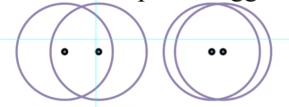
\includegraphics[width=60mm]{img/prox.PNG}
\caption{formato dei messaggi}
\label{fig:form}
\end{figure}
Per la prossimità le due situazioni sono uguali, inoltre non è possibile dire se il secondo sensore è a nord, a sud, a est o ovest dell'altro. 
\bigbreak
La prossimità ci può dare una stima imprecisa di un nodo solo se esistono degli anchor points. Nella figura sopra, pongo che il nodo di sinistra abbia delle coordinate in latitudine e longitudine, il nodo di destra avrà delle coordinate compatibili con quelle. 
\bigbreak
Posso migliorare: se un nodo sente più di un anchor point, posso migliorare la stima della posizione. Più anchor point sento, maggiormente precisa sarà la mia posizione. 
\begin{figure}[h]
     \centering
     \begin{subfigure}[b]{0.3\textwidth}
         \centering
         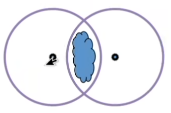
\includegraphics[width=40mm]{img/prox2.PNG}
         \caption{nodo sente due anchor point}
     \end{subfigure}
     \hfill
     \begin{subfigure}[b]{0.3\textwidth}
         \centering
          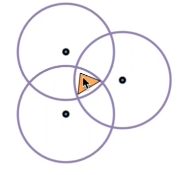
\includegraphics[width=40mm]{img/prox3.PNG}
          \caption{nodo sente tre anchor point}
     \end{subfigure}
    \caption{stima della posizione con più di un anchor point}
    \label{fig:ancopoin}
\end{figure}
\noindent \textit{Una soluzione possibile è usare un solo anchor mobile che si muove nell'area in cui ci sono i sensori ed è dotato di conoscenza della propria posizione assoluta (sono oggetti grossi, posso montarci GPS), esso rileva la presenza di un oggetto e inizia a spostarsi nella sua prossimità. Spostandosi intorno all'oggetto, inizia a restringere l'area in cui l'oggetto si sposta.}

\subsection{Distanza con RSSI}
Posso utilizzare RSSI (Receveid Signal Strength Indicator), misura la potenza del segnale ricevuto. 
\begin{figure}[h]
\centering
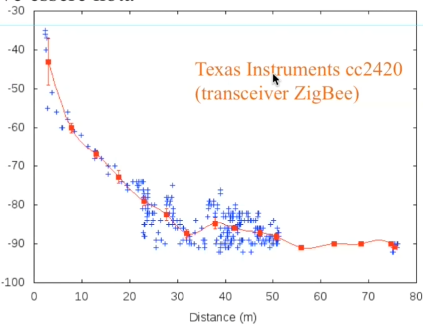
\includegraphics[width=60mm]{img/dist.PNG}
\caption{RSSI - in ascissa distanza dalla sorgente del segnale, in ordinata la potenza del segnale ricevuto}
\label{fig:rssi}
\end{figure}
Ci sono dei problemi, alcune hanno stessa ascissa ma ordinate diverse. Molte crocette sono ad ascissa 22, quindi 22 metri dalla sorgente, ma il segnale viene ricevuto in modo diverso, varie volte. Ricevere a 83 dB mi potrebbe corrispondere ad un range da 22 a 43, a che distanza mi trovo esattamente? 
\begin{itemize}
    \item dipende fortemente da fattori ambientali (multipath fading): il segnale rimbalza in giro e quando viene ricevuto non è una misura effettiva
    \item potenza trasmissiva dev'essere nota (se sento molto una sorgente che emette un segnale debole sono molto vicino, se viceversa sento poco una sorgente con un segnale molto potente, sarò lontano)
    \item la ricezione dipende dall'HW, mi cambia la precisioni di stima della distanza
    \item problemi di stima della distanza, più nodi ricevono il segnale con la stessa potenza, ma i nodi si trovano a distanze diverse dalla sorgente
    \item c'è un decadimento esponenziale, circa come $1/R^2$
    \item dipende da dove sono piazzati i sensori: in guide d'onda $1/R^{1/2}$, siccome il terreno assorbe diventa $1/R^4$
\end{itemize}

\subsection{Distanza TOA/TOF}
Time Of Arrival/Time Of Fligh.

Ragioniamo in una rete wireless, considero due nodi che sono one-hop, posso calcolare il tempo di propagazione. Dal momento in cui viene immesso un bit sul canale, il tempo di propagazione ci indica quanto tempo è stato impiegato perché quel bit sia stato ricevuto dall'altro nodo. 
\bigbreak
Il tempo di propagazione dipende da: velocità di propagazione che è quella della luce per tecnologie wireless e fibra ottica e $2/3$ di $c$ nel rame (ha una resistenza non nulla), e dalla lunghezza del mezzo trasmissivo (nel nostro caso la distanza tra le antenne radio dei due nodi). 
\begin{equation}
    d = t x c
\end{equation}
Avendo già la velocità, devo ottenere il tempo di propagazione. La stazione sorgente emette un beacon a un tempo determinato e il ricevente deve avere un orologio perfettamente sincronizzato con quello della sorgente. A questo punto, quando il ricevente ottiene il beacon sa a che ora gli è stato mandato dalla sorgente e conosce il tempo in cui lo ha ricevuto, facendo la differenza tra i due tempi, posso ottenere il tempo di propagazione. 
\bigbreak
Abbiamo problemi di precisione: è richiesto che gli orologi siano perfettamente sincronizzati e devo calcolare tempi estremamente piccoli. \\ \textit{gli orologi di apparati informatici sono orologi al quarzo, molto precisi ma l'ora dipende dalle vibrazioni di una lamella di quarzo. Innanzitutto sono fatti da madre natura, quindi un cristallo può essere non perfettamente puro, la lamella è fabbricata e questo potrebbe creare altre imprecisioni. Tutto ciò comporta la deriva dei clock: anche se sincronizzo due orologi, nel tempo si sfaseranno.}. 
\bigbreak
\noindent \textbf{Round trip time} \\
\noindent C'è un alternativa, possiamo calcolare il \textbf{round trip time}. Prima misuravamo il tempo di percorrenza in una sola direzione, ora misura il tempo di andata e ritorno. In questo moto diventiamo indipendenti dalla sincronizzazione degli orologi: la sorgente manda un messaggio ad una certa ora, dopo qualche tempo riceve una risposta per quel messaggio, esegue quindi la differenza tra l'ora di ricezione della risposta e l'ora in cui ha mandato la richiesta.  
\bigbreak
Il problema è quando viene mandata indietro la risposta. Sono pacchetti di controllo che non portano in giro dei dati, potrebbe essere che il destinatario decida di occuparsi di altri pacchetti dati e quando non ha nulla da fare, risponde al messaggio per il calcolo del RTT. 

\subsection{Distanza con TDOA}
Time Difference of Arrival. \\ Prendo un HW particolare per cui tutti i nodi hanno un'interfaccia trasmettente e ricevente di due tipi di segnali che vanno a velocità diverse (uno segnale radio a velocità luce, altro a ultra-suoni che vanno a velocità suono). 
\bigbreak
La sorgente fa partire, su entrambe le schede trasmissive, il proprio segnale. Il ricevente riceve i due segnali, prima quello a onde radio e poi quella a ultra-suoni. Il ricevente calcola la differenza tra i due tempi, a questo punto conosce le due velocità di propagazione e il $\Delta$ del tempo di propagazione, la distanza è uguale e quindi può calcolarla. 
\bigbreak
Mi risolve che non devo sincronizzare i clock e calcolare tempi molto molto piccoli (il $\Delta$ tra i due tempi è dell'ordine di $10^3$. I problemi con questa tecnologia sono: l'uso di ultrasuoni che possono infastidire animali e il montare queste interfacce che rende il sensore più "ciaciotto":

\subsection{Angolo - Uniform Linear Array}
Mi serve un array di antenne a distanza fissa e nota una dall'altra. La sorgente emette il segnale che viaggia verso le varie antenne del ricevente. Il segnale percorre distanza diverse a seconda dell'antenna che deve raggiungere. Possiamo così calcolare ciascuna distanza, ed avere una stima della distanza media. 
\begin{figure}[h]
\centering
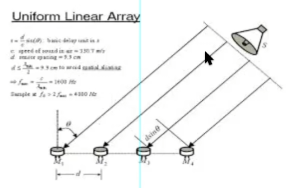
\includegraphics[width=60mm]{img/angolo.PNG}
\caption{Uniform Linear Array}
\label{fig:ula}
\end{figure}

\subsection{Segnali acustici}
Posso usare segnali acustici, non soffrono il multipath fading, hanno un comportamento regolare ($1/R^2$) ma soffrono ostacoli. Gli emettitori/ricevitori sono di grandi dimensioni.

\section{Positioning}
Finora abbiamo visto come calcolare la distanza tra due nodi, ma non abbiamo ancora trovato modi per determinare la topologia della rete né la posizione effettiva dei nodi.
\subsection{Trilaterazione}
Usata in cartografia dal 6° secolo A.C e usato tuttora per GPS. 
\bigbreak
Abbiamo un punto di cui conosco la posizione, anchor point, il sensore - con una delle tecnologie indicate sopra - riesce a calcolare la distanza dall'anchor point, quindi si trova sulla circonferenza. Se calcoliamo la distanza da due anchor point, troviamo che il punto può essere nell'intersezione tra le due circonferenze. Se il nodo riesce a vedere anche un terzo anchor point, ne calcola la distanza, e capisce di essere nell'intersezione delle tre circonferenze. 
\bigbreak
Mi servono tre punti perché ho tre equazioni di secondo grado in due incognite, ogni equazione ci ridà quindi due soluzioni. La terza equazione ci identifica solo una di queste soluzioni. 
\begin{itemize}
    \item richiede calcolo della distanza dagli anchor point
    \item se vogliamo altitudine, passiamo in geometria sferica (interseco 4 sfere) 
    \item devo garantire che ogni nodo senta almeno tre anchor point. \\ Posso, in alternativa, usare un anchor point mobile che si muova sull'area, dotato di GPS, e per ogni nodo misura da tre punti la distanza tra sé e il nodo. 
\end{itemize}

\noindent \textbf{GPS (Global Positioning System)} 
\bigbreak
\noindent GPS utilizza la trilaterazione sfruttando una costellazione di 24 satellite in orbita non geostazionaria per fornire segnale orario e posizione (un satellite in orbita geostazionaria si muove in solido con la terra e il satellite punta sempre sulla stessa porzione di crosta terrestre. Possiamo sempre parlare con lo stesso satellite). Un orbita non geostazionaria è un'orbita bassa, richiede meno batteria e risorse, e non comunichiamo sempre con lo stesso satellite. 
\begin{itemize}
    \item precisione entro 15m il 95\% delle volte
    \item non funziona indoor
    \item costoso in termini di energia: può avere senso non tenere sempre accesso GPS, se i sensori sono fermi lo uso una volta sola, se sono mobili una volta ogni tanto. 
    \item richiede line of sight: il segnale che arriva dal satellite è già debole, se questo incontra ostacoli (pioggia, fogliame, edifici) la ricezione è minima. 
\end{itemize} 
Il ricevente deve riuscire ad individuare 4 satelliti con segnale forte nel proprio "cielo". Una volta trovati questi 4 satelliti, il ricevente li blocca e  deve ricevere le effemeridi da ogni satellite (ora del satellite, forma dell'orbita che sta seguendo e in che posizione è sull'orbita). 
\bigbreak
Le 4 effemeridi sono memorizzate in un almanacco per misure future fino a 2 mesi o se mi muovo in una area di al più 100km, dopo di che il "cielo" è cambiato e devo lockare altri satelliti. 
\bigbreak
Il ricevente calcola il valore medio dei quattro segnali orari che gli arrivano e lo setta come orario proprio. A questo punto viene usata la tecnica TOF (Time of Flight): il ricevitore decodifica l'effemeride di un satellite ed è in grado di capire l'istante di emissione del segnale da parte del satellite, successivamente registra l'ora di ricezione del segnale in base al proprio clock (ottenuto dalla media dei 4 satelliti). Viene calcolata la differenza tra questi tempi e ottiene il Time Of Flight ($d = t*c$) la velocità è nota, il tempo l'ho calcolato - posso calcolare la distanza). Ripeto il calcolo della distanza per i 4 segnali dei satelliti per poter effettuare trilaterazione.

\subsection{Centroide}
Se il GPS non è utilizzabile, posso usare i centroidi. Non mi preoccupo di dover aver una rete di satelliti in orbita, non mi preoccupo di dover piazzare anchor point sul territorio e non mi preoccupo di avere droni, robot mobili sulla superficie in modo che sia possibile stimare la posizione dei sensori. 
\bigbreak
Ipotizziamo di riuscire a vedere delle antenne che periodicamente inviano \textit{beacon} con cui comunicano la propria posizione: 
\begin{itemize}
    \item assumiamo che la propagazione del segnale radio sia ideale, sferica e senza ostacoli (muri, rilievi)
    \item ogni nodo ha lo stesso raggio radio
    \item reference point vicini cercando di de-sincronizzare i propri beacon (per fare sì che il device che si trova nell'area di sovrapposizione tra le due antenne, sente entrambi i beacon e non rumore a causa di interferenza)
    \item non adatto indoor: modello inaccurato a causa di multipath fading. Inoltre si basa sull'assunzione che la propagazione del segnale sia sferica e non ostacolata, indoor ci sono molti ostacoli.
    \item problema: dobbiamo pre-piantare nel terreno gli anchor point. Per accuratezza meglio che essi siano densi, ma la densità porta anche al fatto di dover de-sincronizzare i beacon.
\end{itemize}
Il metodo del centroide usa il metodo della prossimità. Il device sente le antenne intorno a lui e stima l'area in cui si trova, la posizione corrisponde al baricentro. 
\bigbreak
Un problema potrebbe essere che il device può sentire anche beacon di antenne che non sono effettivamente nel suo raggio radio e spostano la posizione apparente del nodo (a causa di guide d'onda ad ex). Devo capire quali antenne sono land-mark, cioè antenne significative per la stima della posizione (ad ex. se sento un segnale debole probabile che l'antenna non sia molto significativa). 
\bigbreak Il device cerca di capire chi e quante antenne sente, per fare ciò raccoglie campioni. Il device aspettare un tempo sufficiente al land-mark per mandare S campioni, conto che il land-mark manda un campione ogni periodo T. 
\begin{equation}
    t = (S + 1 + \epsilon)T
\end{equation}
In teoria, nella situazione ideale, potrebbe bastare $t = S*T$, in realtà ci sono una serie di problemi che mi portano ad aggiustare l'equazione. Aggiungo 1 per ovviare alla situazione in cui il device si mette in ascolto un attimo dopo che il primo beacon è stato mandato, quindi deve aspettare T per vedere il primo e 2T per vedere il secondo. $\epsilon$ viene aggiunto ad ex. per problemi di sincronizzazione tra orologi. 
\bigbreak
Per il tempo $t$, il nodo che vuole determinare la propria posizione, ascolta tutti i beacon che riesce a raccogliere, questi gli permettono di sapere quali anchor point vede. Per ogni sorgente segna che ha ricevuto dei beacon e quanti ne ha ricevuto nel periodo $t$. Dopo ciò compie una selezione, sceglie gli anchor point di cui, nel periodo $t$, ha sentito almeno il 90\% del beacon. Questi diventano i reference point del nodo.La posizione del nodo è il baricentro, posizione media, dei reference point che il nodo ha scelto nella selezione effettuata prima.
\bigbreak
Sperimentalmente funziona: con 20 campioni sentiti dagli anchor point, l'errore medio è sotto i 2 metri. 

\subsection{Fingerprint - Signal Pattern Rematching}
Vengono pre-piazzati dei dispositivi, anchor point che mandano i loro beacon. In questo caso non mi interessa che nei beacon sia presente la posizione dei device, gli anchor point mandano solo il proprio identificativo. 
\bigbreak
La superficie di interesse è mappata tramite una griglia, in ogni punto di intersezione piazzo un dispositivo, uguale a quelli di cui devo trovare la posizione, che registra gli anchor point che sente e la potenza del segnale in quel punto (RSSI). All'ingresso dell'area metto un totem, gli utenti scaricano da questi la mappa e i fingerprint dei vari punti di intersezioni della mappa. Una volta che gli utenti entrano nell'area considerata, il dispositivo utente registra i beacon e la potenza degli anchor point che vede. A questo punto posso paragonare ciò che vede il dispositivo utente alle finger print dei punti di intersezione, sono in prossimità del punto più simile alle mie caratteristiche. 
\bigbreak
\noindent In alternativa, possiamo sfruttare prossimità con dispositivi a raggio breve (RFID). Ad ex. dispositivi a infrarossi che non superano i muri, questo mi consente di capire in che stanza mi trovo

\chapter{VANET - vehicular ad hoc networks}
Bibliografia - si trovano in lezione e materiali didattici: 
\begin{itemize}
    \item[-]S. Al-Sultan, M.M. Al-Doori, A.H. Al-Bayatti, H.Zedan
    \textit{A comprehensive survey on veichular ad hoc networks - pp. 380-392}
    \item[-]D.Jiang, L.Delgrossi
    \textit{towards an international standard for wireless access in vehicular environments - pp. 2036-2040}
\end{itemize}
Rete costituita da dispositivi wireless a bordo di veicoli (ed eventuali apparati a lato strada). 
\bigbreak
\noindent \textbf{Intelligent Transport System (ITS)} 
\bigbreak
\noindent Integrazione delle conoscenze nel campo delle telecomunicazioni, elettronica e informatica con l'ingegneria dei trasporti per la pianificazione e la progettazione dei sistemi di trasporto.
\begin{itemize}
    \item Comunicazione in-vehicle (oggetti sul veicolo: sensori di parcheggio, altoparlanti bluetooth, sensori che non hanno bisogno di comunicare all'esterno).
    \item comunicazione tra i veicoli (auto-veicoli, macchine industriali che sanno comunicare e cooperare per svolgere i propri compiti). 
    \item comunicazione tra veicoli e infrastruttura 
\end{itemize}
Infrastruttura VANETs:
\begin{itemize}
    \item AU (Application Unit): apparati a bordo che implementano applicazioni per veicoli e passeggeri 
    \item OBU (On Board Unit): sono a bordo, comunicazioni sui veicoli per comunicare con altri veicoli e unità lato strada. Sono usate da AU per mandare dati ad altre macchine, sono responsabili di gestione di mobilità e networking. 
    \item RSU (Roadside Unit): sono unità fisse a lato strada, non hanno problemi di mobilità, danno connessione ad Internet ed estendono range di comunicazione tra veicoli (due veicoli potrebbero non essere nello stesso raggio radio, il veicoli davanti potrebbe lasciare informazioni alla RSU quando le passa vicino e la RSU scarica le informazioni sul veicolo che passa successivamente). 
\end{itemize}

\noindent Domini di comunicazione:
\begin{itemize}
    \item[-] comunicazione in-vehicle: comunicazione tra sensori e parti del veicolo (AU), sfruttando OBU. Sfrutta tecnologie a corto raggio: wireless USB, ZigBee. 
    \item [-] comunicazione ad hoc: comprende due tipi di infrastutture: V2V (vehicle to vehicle) cioè comunicazione tra OBU e V2I (vechicle to Infrastracture) cioè comunicazione tra OBU e RSU. Solitamente vengono utilizzate tecnologie WiFi (IEEE 802.11p, tecnologia creata apposta).
    \item [-] comunicazione infrastrutturale: connessione di RSU o OBU a Internet, usano tecnologie 3G, 4G, WiMax. 
\end{itemize}

\noindent \textbf{Standard 802.11} 
\bigbreak
\noindent Insieme di standard di trasmissione per reti WLAN, sviluppato dal gruppo 11 dell'IEEE 802, con particolare riguardo al livello fisico e MAC, specificano sia l'interfaccia tra client e base station (o access point) sia le specifiche tra client wireless. 
\bigbreak
Nell'infrastruttura VANET abbiamo comunicazione V2V o V2I, la prima è una rete completamente mobile mentre la seconda è più simile a una WiFi con un Access Point a cui gli apparati si connettono. \\ Questi gruppi che stanno sotto un AP vengono definiti dall'antenna stessa, tramite due identificatori SSID e BSSID. Il primo è un nome che specifica cosa accade nel gruppo (ex. parcheggi disponibili nel quartiere), il secondo è il MAC address dell'antenna che fa da AP. \\ Normalmente è l'antenna l'iniziatore del gruppo, i device utente vedono che gruppi esistono e decidono se aderire o meno. 
\bigbreak
Un gruppo di può estendere su più celle: gli AP devono farsi carico di passare traffico dagli utenti che stanno in una cella fino agli altri. \\ Inoltre è possibile creare gruppi ad-hoc senza AP fisso costituiti unicamente da apparati utenti, in questo caso l'identificativo è IBSS e un BSSID casuale. L'iniziatore di un gruppo ad hoc genera un numero casuale e lo usa come BSSID del gruppo
\bigbreak
In una rete di questi tipi, se l'iniziatore si sposta o si spegne, l'intero gruppo cessa di esistere e i device in quella cella non possono più parlare. \\ C'è un'eccezione in cui è possibile usare una \textbf{wildcard BSSID} (con 48 bit a 1) per creare un gruppo, ma è usato solo per gestione (coordinamento degli AP).
\bigbreak
Il problema di usare 802.11 nelle VANET è importante: ci vuole troppo tempo per realizzare i gruppi, per far scoprire al device utente che gruppi esistono, per prendere BSSID e SSID, per decidere come farlo parlare sul canale fisico sincronizzandosi con gli altri. 

\section{Standard 802.11p WAVE} 
La mobilità richiesta dalle VANET è considerevole: gli apparati hanno una velocità non trascurabile, le velocità relative dei mezzi sono ancora maggiori e conseguentemente ci sono molti cambi nella topologia di rete. \\
Per rispondere a queste nuove necessità, si sono cercate nuove soluzioni: nel 1999 negli USA,  hanno incominciato a capire come far funzionare un livello fisico e MAC dedicato alla sicurezza stradale, lo hanno chiamato Dedicated Short Range Communication (DSRC). Questo si occupa di comunicazione a corto raggio, come su veicoli sulla stessa strada o veicoli che scambiano informazioni con un apparato a lato strada. Successivamente la ricerca viene estesa fuori dagli Stati Uniti e nasce uno standard internazionale, 802.11p WAVE (Wireless Access in Vehicular Environments). 
\bigbreak
WAVE individua un particolare standard dialetto di 802.11 che doveva andare bene per reti veicolari, particolarmente a livello fisico e livello MAC, sono state eliminate alcune caratteristiche di 802.11 che richiedevano alta latenza e ritardi. \\
Funziona nello spettro dei 5.9 Ghz, banda classificata come "free but licensed": chiunque può produrre dispositivi che emettono in questo range senza pagare un fio annualmente, ma tutti quei dispositivi devono avere una licenza. La licenza è fornita da un comitato internazionale che controllo che il dispositivo sia conforme allo standard WAVE. 
\bigbreak
Il canale fisico di WAVE si compone di 7 sotto-canali, ognuno con un'ampiezza di 10MHz:
\begin{figure}[h]
\centering
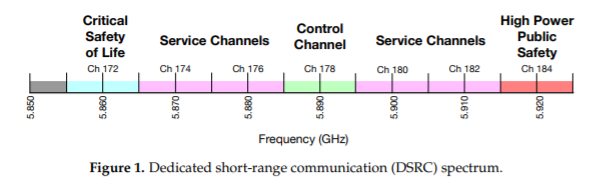
\includegraphics[width=100mm]{img/wavespec.PNG}
\caption{Divisione in 10MHz}
\label{fig:ulfrfrwar}
\end{figure}
\begin{itemize}
     \item [-] canale 178 - canale di controllo: usato solo per comunicazioni di safety, è l'unico canale accessibile da tutti in qualunque momento perché tutti sono già nel canale senza dover accedervi o configurarsi.
    \item [-] canale 172 - canale di safety: comunicazione a corto raggio per messaggi critici per la sicurezza (evitare una collisione tra due veicoli vicini)
    \item [-] canale 184 - canale di safety: comunicazione per la sicurezza del traffico tipicamente multi-hop (segnalare che si sta avvicinando ad un incrocio o l'arrivo dell'ambulanza e quindi bisogna spostarsi)
    \item [-] canali rosa: applicazioni utente che non hanno a che vedere con sicurezza del traffico (pubblicità, entertainment, giochi, cose commerciali)
\end{itemize}
Per accedere un canale in 802.11 normali ho bisogno di tempo: devo scambiare beacon, capire chi ho intorno, capire come accedere al canale (FHSS, DHSS) etc. Non posso permettermelo in comunicazioni di safety (non posso aspettare secondi prima di segnalare un incidente), per fare questo tutti i veicoli devono essere già connessi al canale di controllo 178 e, perciò, devono avere radio multiple (una radio sempre sintonizzata sul canale di controllo e le altre su altri canali)
\bigbreak
Esiste una \textbf{wildcard BSSID} in WAVE che non è utilizzata esclusivamente per gestione come in 802.11. In WAVE è usata per consentire sempre a tutti, in qualunque momento, l'accesso al canale di controllo 178. Tutti gli apparati di una rete WAVE avranno perennemente una radio sintonizzata sul canale 178. 
\bigbreak
Gli altri canali funzionano con BSSID più simili a 802.11 ma non uguali, chiamati WBSSID. L'idea è che ogni nodo in una WBSSID periodicamente manda un SOLO beacon con informazioni sui contenuti scambiati e sui servizi offerti nel gruppo e con informazioni utili per fare configurazione di canale per entrare nel gruppo (senza ulteriore negoziazione di parametri, come in 802.11, per permettere al nodo di entrare).\\ Ci va molto bene 

\section{Caratteristiche delle VANET}
\begin{itemize}
    \item mobilità caotica: vincolata dalla topografia delle strade (in autostrada andrà in linea retta, negli edifici non si passa e viabilità, segnali stradali). 
    \item velocità alte, specie quelle relative tra veicoli
    \item non abbiamo problemi di batteria e memoria: le prime si ricaricano andando e ho abbastanza spazio per montare CPU e memorie grandi
    \item alto numero di dispositivi ($10^3$, $10^4$)
    \item densità variabile in funzione delle condizioni del traffico
    \item bilanciamento tra connettività e contesa: posso trasmettere con potenza maggiore ma creo contesa tra maggior numero di nodi (in una rete densa possiamo decidere di usare una potenza radio bassa in modo che il segnale non venga sentito molto lontano, ma essendo densi lo sentono comunque ma creo meno collisioni. In una rete sparsa alzo la potenza così da raggiungere più nodi)
    \item disponibilità informazioni di locazione (GPS)
\end{itemize}

\noindent Requisiti delle applicazioni
\begin{itemize}
    \item comunicazioni d'emergenza: sono le più toste perché hanno due requisiti in contrasto uno con l'altro. Il primo requisito è che i dati vengano trasmessi affidabilmente e il secondo è che questo avvenga con bassa latenza (se voglio affidabilità ho bisogno di tempo, ma così alzo la latenza. Inoltre il canale wireless ha un bit error rate più alto delle reti fisse in generale e il fatto che sia broadcast porta anche a collisioni, tutto ciò va contro l'affidabilità e garantire l'affidabilità aumenta la latenza).
    \item privacy: dati sul movimento dei veicoli possono dischiudere informazioni sensibili ("il veicolo XXX va spesso nel quartiere a luci rosse").
    \item scalabilità
\end{itemize}

\subsection{Pattern di comunicazione:}
\begin{itemize}
    \item unicast: indirizzando specifico destinatario
    \item multicast/anycast: ci sono due alternative possibili
         \begin{itemize}
             \item [-] indirizzamento di gruppo IP-like
             \item [-] indirizzamento guidato da contenuto (data centrico) o tipo veicolo (tutte le pattuglie in zona XXX, qualunque ambulanze a distanza inferiore a 10 metri)
         \end{itemize}
        Con multicast intendiamo il far recapitare il messaggio a tutti i componenti di un gruppo,a priori i nodi che vogliono ricevere una particolare tipologia di traffico, si registrano in uno specifico gruppo. \\ Con anycast intendiamo diffondere il messaggio a qualcuno: per alcune applicazioni è sufficiente mandare un dato, non a tutti i membri di un gruppo, ma ad uno solo qualunque dei membri di quella comunità (non vogliamo chiamare tutte le ambulanze in zona, ce ne basta una sola). \\ Fare ciò IP-like è scomodo, dovrei pre definire i membri di un gruppo (ma se c'è un incidente, non so che macchine passeranno di lì). E' più comodo un approccio basato sul contenuto, i veicoli ad una distanza minore di tot metri dal punto considerato. 
    \item \textbf{geographic routing}: unicast, trovare il percorso verso un nodo che si trova in determinate coordinate geografiche (non usando l'indirizzo IP)
    \item \textbf{geocast}: multicast, sono interessata a mandare un dato ad un insieme di nodi che sono identificati come destinatari dal fatto che si trovano in una determinata area 
\end{itemize}

\chapter{Location Service}
Bibliografia - si trovano in lezione e materiali didattici: 
\begin{itemize}
    \item[-]J. Li, J.Jannotti, D.S.J. De couto, D.R.Karger
    \textit{A scalable Location service for geographic ad hoc routing}
\end{itemize}
Servizio che permette, in modo distribuito, ai nodi delle rete di localizzare gli altri nodi della rete. 
\bigbreak
Gli algoritmi di routing (AODV) per MANET sono poco efficaci, alto overhead (monitoring continuo, flooding) e informazioni presto obsolete (alta mobilità, i percorsi trovati e che devono essere percorsi a ritroso spesso scompaiono dopo poco).
\begin{figure}[h]
\centering
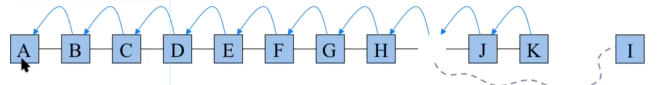
\includegraphics[width=90mm]{img/aodv.PNG}
\caption{percorso interrotto}
\label{fig:perinte}
\end{figure}

Quello che possiamo osservare è che abbiamo un problema se si parlano due nodi lontani, se guardiamo a breve distanza - devono parlare A, B,  ad ex - ho meno complicazioni. Inoltre un nodo non sa cosa sta succedendo lontano da lui, ma conosce la situazione dei suoi vicini. C'è una sorta di effetto relativistico: tanto più lontano è un nodo, tanto più è obsoleta e imprecisa l'informazione. \\ \textbf{La precisione con cui la posizione di una destinazione dev'essere nota per prendere decisioni di routing dipende dalla distanza.} \\Possiamo anche però osservare che non siamo interessati ad avere informazioni estremamente precise sulla topologia della rete anche in punti remoti di essa (so che un veicolo era in un quartiere, arrivo fino là e poi chiedo esattamente in che via trovare quel veicolo). 
\bigbreak
Con alta mobilità non ha senso costruire una conoscenza totale di topologia, la quale cambia molto spesso. Allora l'idea potrebbe essere questa: un nodo prende l'informazione più recente sulla posizione della destinazione e guarda i propri vicini per scegliere quello più vicino alla posizione della destinazione. Il nodo scelto è un poco più vicino alla destinazione del nodo iniziale, guarda i suoi vicini e sceglie quello più vicino alla destinazione e così via. 
\bigbreak
\noindent Caratteristiche innovative del routing:
\begin{itemize}
    \item [-] on demand (reattivo): questo protocollo non scambia periodicamente vettori di distanza per avere già rotte, nel momento in cui un nodo ha un dato da spedire il protocollo si preoccupa di come instradare. 
    \item [-] non vengono costruite rotte intere: un nodo guarda solo lo stato locale e i suoi vicini quando ha un messaggio da inoltrare (non quando una sorgente da qualche parte della rete genera un messaggio, ma solo quando questo messaggio arriva al nodo intermedio)
    \item [-] conoscenza delle caratteristiche dei vicini: dove stanno, dove vanno (posizioni, interessi), chi frequentano (devo mandare un messaggio a qualcuno in Città Studi, lo inoltro ad un mio vicino che frequenta spesso quella zona).
\end{itemize}

\section{Geographic forwarding}
Non parliamo di routing, routing consiste nel trovare una rotta valida, corretta e senza loop. Parliamo di forwarding perché in queste reti non esiste una rotta, è un inoltro locale di ciascun nodo verso un altro.
\begin{figure}[h]
\centering
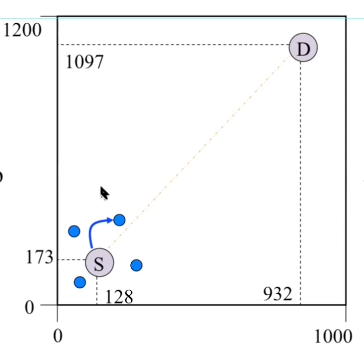
\includegraphics[width=60mm]{img/geofor.PNG}
\caption{percorso interrotto}
\label{fig:geofor}
\end{figure}
\bigbreak
In figura, copriamo un'area di circa 1000km. La sorgente S genera un messaggio per la destinazione D. Dobbiamo scoprire a che coordinate si trovava D l'ultima volta, la sorgente S conosce solo i suoi vicini (tramite beacon condividono la loro posizione), sapendo come sono piazzati i suoi vicini sa scegliere quello più vicino a D. \\ Può darsi che i vicini di S siano mobili, il segnale viaggia alla velocità della luce e i vicini sono in prossimità, riusciamo a battere il problema della mobilità. 
\begin{itemize}
    \item Mano a mano che ci allontaniamo dalla sorgente troveremo delle informazioni più recenti e corretti riguardo alla posizione di D, aggiustiamo la rotta mano a mano che ci avviciniamo alla destinazione
    \item  Le decisioni sono chiaramente locali, la vista di ciascun nodo e le sue decisioni sono limitate ai suoi vicini one-hop.
    \item L'approccio di questo algoritmo è store and forward (come i ruoter in Internet, memorizzo il pacchetto e guardo a chi inoltrarlo): se un nodo non trova un vicino in posizione migliore della propria rispetto alla destinazione, butta via il messaggio
\end{itemize}
Quando scelgo il next-hop posso fare una scelta che consideri anche la topografia: i veicolo sono solo nelle strade (se un vicino di S è sulla strada retta che conduce a D, potrebbe essere la scelta migliore. Ma devo considerare che le strade potrebbero non essere dritte: anche se un vicino è più prossimo alla linea retta che congiunge S a D, devo valutare la topografia delle strade e la direzione dei nodi vicini). 
\bigbreak
C'è un altro tipo di problema: se non ci sono vicini in posizione migliore, il pacchetto viene buttato via. 
\begin{itemize}
    \item posso usare qualche tecnica per trovare una rotta sub-ottima, che è una rotta peggiore (viene scelto un vicino magari più lontano) ma spero che prima o poi si arrivi a destinazione
    \item posso passare ad un paradigma store, carry and forward. Il nodo non butta via il pacchetto né sceglie qualcuno che è peggio di lui, questo approccio usa la mobilità. Il nodo tiene il pacchetto e muovendosi può succedere che, in futuro, si trovi in una posizione migliore e a quel punto inoltra il pacchetto. \\Queste sono dette reti opportunistiche, il nodo inoltra il messaggio quando incontra un nodo che ha più probabilità di lui di far arrivare il pacchetto a destinazione. 
\end{itemize}

\section{Location service}
Servizio che consente ad un nodo di scoprire le coordinate di un altro nodo (devo scoprire le coordinate della destinazione D)
\begin{figure}[h]
\centering
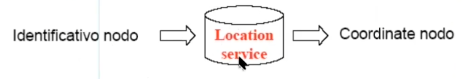
\includegraphics[width=90mm]{img/locserv.PNG}
\caption{location service come blackbox}
\label{fig:locser}
\end{figure}
\bigbreak
Sembra un DB, esegue una query e ricevo una risposta. Non posso avere un DB centralizzato, perché sarebbe un approccio fragile (bottleneck, single point of failure). 
\bigbreak
Noi sappiamo trovare la posizione locale di un nodo: GPS, trilaterazione con anchor point, beacon per conoscere i vicini. Ma qui si tratta di un nodo che ha bisogno di conoscere le coordinate di un altro nodo della rete. 
\bigbreak
\noindent Sia il geographic forwarding che il location service hanno bisogno di un assunto:
\begin{itemize}
    \item assunzione di mobilità: i dati si muovono più velocemente dei nodi. Se così non fosse la consegna sarebbe impossibile: la sorgente S manda un messaggio a D, ma D si sta spostando. Per consegnare stiamo inseguendo D, considerando valida l'assunzione, i messaggi sono sempre più vicini alla destinazione, anche se questa si sta spostando. 
    \item dovrei anche assumere che un nodo che è in un parte della rete, non compaia improvvisamente dall'altra parte della rete (non è sempre valido perché un nodo potrebbe spegnere la radio, diventando invisibile, e riaccenderla nella parte opposta della rete). 
\end{itemize}
L'assunzione di mobilità, nelle sue due declinazioni, va bene per le VANET (la prima declinazione è soddisfatta e per la seconda, non avrebbe senso spegnere la radio, la batteria è potente). 

\subsection{Richiamo su modelli di mobilità}
Si usano due modelli semplici:
\begin{itemize}
    \item Random Walk: nodo si muove in direzione casuale, per un certo tempo o fino a coprire una certa distanza. Una volta terminato il moto, viene ripreso in un'altra direzione casuale. \\ E' un moto casuale e caotico. Se un nodo urta un confine quando ancora non ha finito il moto può: rimbalzare (i veicoli non lo fanno) o peggio re-ingresso nel lato opposto (nemmeno questo è fatto dai veicoli). \\ Inoltre potrebbe darsi che un nodo stiamo sempre intorno al punto iniziale. \\ E' un moto facile da descrivere statisticamente ma poco realistico.
    \item Random Waypoint: nodo sceglie punto di arrivo a caso, e si muove in linea retta verso di lui a velocità stabilità. Terminato il moto, c'è un tempo di attesa prima di generare un nuovo punto di arrivo e una nuova velocità. \\ Non ci sono confini, tutti i punti di arrivo sono all'interno della superficie. E' meglio distribuito sull'area rispetto a RW. 
\end{itemize}
Ma vanno bene questi modelli? Gli umani si muovo randomicamente? \\
Sono stati fatti dei modelli più realistici, tengo conto delle code sulle strade, tengo conto che alcuni veicoli possono superarsi e si possono incontrare semafori. Posso anche tenere conto di traiettorie regolari (i mezzi pubblici ad ex.).

\subsection{Soluzione statica per location service}
Ogni nodo della rete ha una posizione home (un access point vicino al garage di casa o lavoro). La home mantiene informazioni aggiornate sulle posizioni dei suoi nodi. 
\begin{figure}[h]
\centering
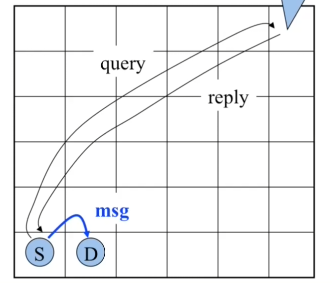
\includegraphics[width=50mm]{img/home.PNG}
\caption{griglia home}
\label{fig:home}
\end{figure}
\bigbreak
Ogni quadratino in figura corrisponde a una home, in questa tipologia di soluzione all'interno di ogni quadratino c'è un'antenna responsabile dei nodi all'interno del quadratino: i nodi comunicano alla home qual è la loro nuova posizione quando si spostano. Una sorgente che deve parlare con una destinazione, determina qual è la home della destinazione tramite funzione di hash (mi permette di distribuire il carico di lavoro sulle celle, antenne). 
\bigbreak

Problemi: 
\begin{itemize}
    \item [-] soluzione centralizzata: se cade l'antenna non ho più informazioni dei nodi che la usano come home
    \item [-] costo scorrelato dalle posizioni: in figura S e D sono in celle vicine, ma la sorgente deve mandare una richiesta fino alla home in alto a destra per poi accorgersi che D era molto vicino a lei
\end{itemize}
C'è un modo di renderlo distribuito, i nodi all'interno di una cella mantengono informazioni su tutti i nodi che entrano nella cella (ma ci dev'essere sempre almeno un nodo in ogni cella)

\subsection{Soluzione triviale per location service}
Non riusciamo a risolvere i problemi della soluzione statica, ricorriamo al \textbf{flooding}. Non scegliamo un'antenna che mantiene informazioni di nodi, vogliamo che tutti mantengano informazioni di tutti.
\begin{itemize}
    \item position query: chiediamo a tutti se conoscono la posizione della nostra destinazione (molto costoso)
    \item position updates: ogni volta che un nodo si sposta in modo significativo (parametro a scelta dell'algoritmo) quel nodo comunica a tutti nella rete dove si è spostato (con mobilità alta flooding continui ed inutili)
\end{itemize}

\section{Soluzione GLS per location service}
Per ogni nodo c'è un pool di location service che conosce la sua posizione nel sistema. Questo garantisce robustezza (un server si guasta non è un problema), inoltre questi server sono anche scelti con un criterio in modo che nessun server sia sovraccarico di nodi da gestire e con un criterio geografico, in modo che un nodo possa trovare un location server vicino a me per qualunque destinazione.
\bigbreak
\noindent \textbf{Goal:} ricerche di un nodo vicino devono trovare risposta nel vicinato
\bigbreak
\subsection{Assunzioni e osservazioni}
\noindent Assunzioni:
\begin{itemize}
    \item [-] ciascun nodo sa fare inoltro geografico per qualunque cosa (query di locazione, reply se è location server di qualunque, location update e dati delle applicazioni). Non è un'assunzione difficile
    \item [-] routing su piccola area intorno ad un nodo (un nodo conosce i suoi vicini 2-hop, ad ex. con approccio distance vector). Posso parlare di routing, creo delle piccole rotte (per farlo, quando mando i beacon carico anche i beacon dei miei vicini. Non è molto difficile)
    \item [-] conoscenza comune di griglia sovrimposta all'area (possiamo mettere RSU che scaricano sul navigatore delle macchine le informazioni della griglia, non molto difficile). 
    \item [-] clock sincronizzati (è presente GPS, non molto difficile da ottenere)
    \item [-] nodi densi, in modo che non ci siano partizioni e massimi locali (in realtà non è un evento molto probabile). 
\end{itemize}
\bigbreak
\noindent Osservazioni:
\begin{itemize}
    \item [-] l'assunzione (c) è risolta scaricando la griglia all'ingresso dell'area urbana
    \item [-] la griglia è \textbf{gerarchica}: abbiamo la nostra area relativa che parte da un'origine che decidiamo noi. La gerarchia nasce ora, il quadrato totale è diviso, con granularità più fine, in quadrati di ordine 1. Poi ripartendo dall'origine i quadrati di ordine 1 sono raccolti in gruppi di quattro (due per ascisse che aumentano, due per ordinate che aumentano). Quattro quadrati di ordine uno diventano un quadrato di ordine 2, ripartendo la stessa operazione quattro quadrati di ordine 2 formano un quadrato di ordine 3, così fino a che non copriamo tutta l'area.
    \begin{figure}[h]
    \centering
    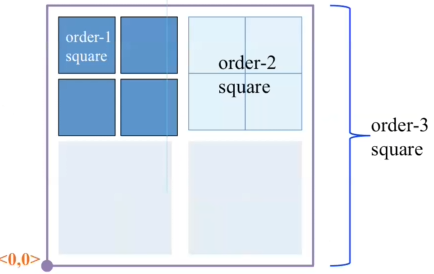
\includegraphics[width=55mm]{img/gergrid.PNG}
    \caption{griglia gerarchica}
    \label{fig:home}
    \end{figure}

    \item [-] l'assunzione (b) è risolta prendendo i quadrati di ordine 1 con un lato tale per cui i due nodi più lontani nel quadrato (sulla diagonale) siano al più a distanza due-hop (considero la tecnologia radio che uso, 802.11p ha un raggio in condizioni ideali di 300m, prendo una diagonale al più di questa distanza) 
\end{itemize}

\noindent \textbf{Come piazziamo i location server? come li aggiorniamo quando il nodo si sposta? come fanno i nodi a trovare le informazioni di locazioni di altri nodi?} 

\subsection{Operazioni}
\noindent \textbf{Operazioni in un quadrato di ordine 1} 
\bigbreak
Ogni coppia di nodi nello stesso 1-quadrato è a distanza massima di due-hop: le tecnologie wireless usano un beacon periodico, con il quale il nodo manda il proprio ID e la propria posizione (in VANET ottenibile da GPS). Ciascun nodo può aggiungere al beacon l'ID e la posizione dei propri vicini, così ogni nodo conosce ID e locazione di ogni altro nodo nel proprio 1-quadrato. 
\bigbreak
\noindent \textbf{Lemma 1:} se query da sorgente S per destinazione D, con S e D nel medesimo 1-quadrato, allora query arriva a D in 1 step
\begin{itemize}
    \item [-] Se D è un vicino di S: la sorgente ha ricevuto il beacon e ha già un cammino. 
    \item [-] Se D è a 2-hop da S: la destinazione ha mandato i beacon ai suoi vicini, basta che la sorgente ne abbia ricevuto almeno uno. Nel caso peggiore sono due periodi di aggiornamento di beacon
    \item[-] Se sorgente deve trovare una destinazione vicina, non succede che deve chiedere ad un location server lontano per poi tornare indietro
    \item[-] Uno step (passaggio da sorgente al relay1, al relay i al relay i+1 fino ad arrivare alla destinazione) può essere formato da più di un hop.
\end{itemize}

\noindent \textbf{Operazioni in un quadrato di ordine k$>$1} 
\bigbreak
 Questo mi racchiude più di una situazione: i nodi possono essere in due 1-quadrati diversi ma nel medesimo 2-quadrato (in nero in figura), oppure due nodi in due 1-quadrati diversi in due diversi 2-quadrati ma che sono nello stesso 3-quadrato (in rosso in figura).
\begin{figure}[h]
\centering
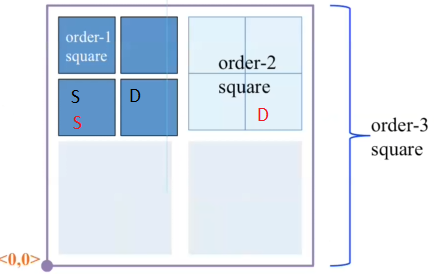
\includegraphics[width=50mm]{img/gergridmod.PNG}
\caption{diverse situazioni}
\label{fig:home}
\end{figure}
Un nodo che mette le proprie informazioni di locazione sui location server non sa chi siano i proprio LS e un nodo che cerca informazioni su un nodo D, non sa chi siano i LS della destinazione D. 
\bigbreak
Il goal è il costo per trovare un nodo sia proporzionale alla distanza tra chi lo cerca e il nodo stesso, dobbiamo piazzare LS a varie distanza dal nodo in modo tale che sorgenti vicino al nodo trovino LS vicini e sorgenti lontane dal nodo trovino LS nel loro vicinato o non oltre la distanza tra sorgente e destinazione.
\bigbreak
\noindent \textbf{Per ogni k-quadrato in cui si trova il nodo n $\longrightarrow$ il nodo mette un LS in ogni (k-1)-quadrato, appartenente al k-quadrato, in cui il nodo non si trova}
\begin{figure}[h]
     \centering
     \begin{subfigure}[b]{0.4\textwidth}
         \centering
         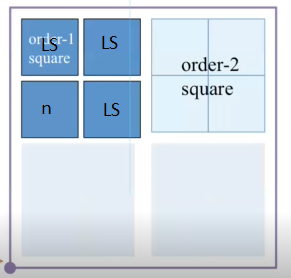
\includegraphics[width=40mm]{img/gridgerls2.PNG}
         \caption{k=2: n mette un LS in ogni 1-quadrato in cui non si trova}
     \end{subfigure}
     \hfill
     \begin{subfigure}[b]{0.4\textwidth}
         \centering
          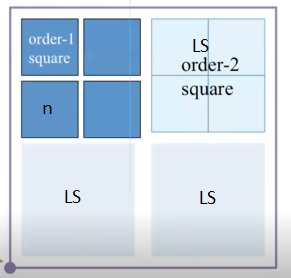
\includegraphics[width=40mm]{img/gridgerls3.PNG}
          \caption{k=3: n mette un LS in ogni 2-quadrato in cui non si trova}
     \end{subfigure}
    \caption{rappresentazione grafica della locazione dei LS}
    \label{fig:gewgnmer}
\end{figure}
\bigbreak
\noindent Il location server di \textit{n} in un k-quadrato è il nodo con ID più vicino a \textit{n} con ID $>$ ID(\textit{n}), tra tutti quelli nel quadrato. Stiamo assumendo che ci siano ID completamente ordinabili, considero l'ordinamento circolare: quando arrivo al più grande ma ho bisogno di un LS, il LS diventa il più piccolo. 
\newpage
\begin{figure}[h]
\centering
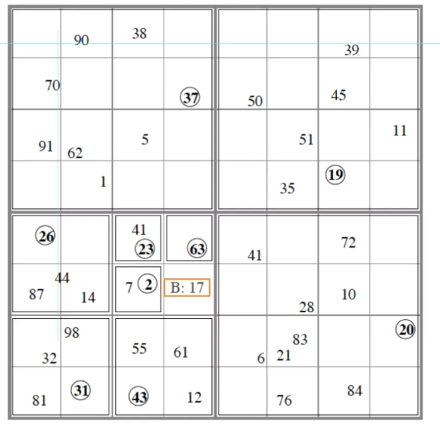
\includegraphics[width=60mm]{img/LSex.PNG}
\caption{esempio posizione LS}
\label{fig:hhtrhrt}
\end{figure}
\noindent Stiamo considerando il nodo B:17. Questo nodo deve avere un LS in ogni 1-quadrato del 2-quadrato in cui si trova. 
\begin{itemize}
    \item [-] 1-quadrato in alto a dx ha LS = 63 perché è l'unico presente
    \item [-] 1-quadrato in alto a sx ha LS = 23 perché è il più piccolo dei maggiori di 17
    \item [-] 1-quadrato in alto a sx ha LS = 23 perché è il più piccolo maggiore di 17
\end{itemize}
Non abbiamo bisogno di far conoscere ai nodi i LS di un nodo \textit{n}, nemmeno ad \textit{n} stesso. L'assunzione (a) ci garantisce che ogni nodo sappia fare inoltro geografico e l'assunzione (c) mi garantisce che la griglia sia condivisa. \\ Poniamo caso, nell'esempio sopra, che il nodo B debba mandare un update di posizione nel 3-quadrato in alto a sx e quindi trovare il LS, non ha però idea di che nodi si trovino al suo interno. Il nodo B manda l'update alle coordinate (tramite inoltro geografico (a) ) al baricentro del 3-quadrato (B conosce il baricentro perché la griglia è condivisa (b) ). 
\bigbreak
L'inoltro geografico verso il baricentro del quadrato in cui LS deve risiedere, passa per i nodi vicini a B: B manda l'update al nodo 23, al nodo 41, al nodo 1 e qui si ferma. Il nodo 1 vede che sta inoltrando un pacchetto di location update per un 3-quadrato in cui lui si trova. 
\bigbreak
I location update sono inoltrati geograficamente anycast (basta prendere un qualunque nodo all'interno del quadrato target). Quando ho trovato almeno un nodo, questo nodo (il nodo 1 nell'esempio) incapsula il location update in un messaggio che sembra una query (\textit{fake query}) per trovare il LS di B. La query cerca il LS inizialmente nell'1-quadrato, se non lo trova cerca nel 2-quadrato e così via finché non lo trova. La query si ferma perché contiene un'informazione che dice di cercare il LS in k-quadrato, 3-quadrato nell'esempio, quando la query dovrebbe entrare nel 4-quadrato, si ferma.

\subsection{Diffusione della query}
\begin{figure}[h]
\centering
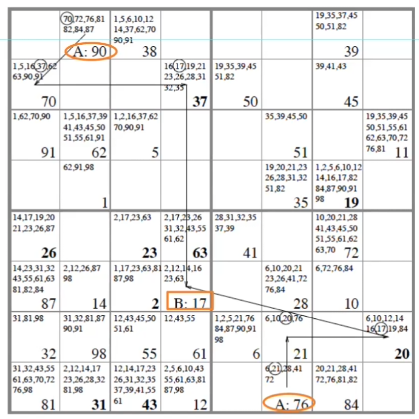
\includegraphics[width=60mm]{img/diffqueryls.PNG}
\caption{esempio diffusione query}
\label{fig:hhtrhrffrt}
\end{figure}
La figura è semplificata: in ogni quadrato vediamo un nodo solo, le scritte indicano per quali nodi fa da LS. 
\bigbreak
Un nodo, ad ex A:90, vuole mandare un pacchetto al nodo B:17, prima di tutto, deve arrivare a conoscere la posizione del nodo B.
\begin{enumerate}
    \item il nodo A guarda se B è nel suo 1-quadrato (conosce tutti i nodi all'interno del suo 1-quadrato, per il lemma 1 ci metto solo 1 step)
     \item il nodo A non è all'interno, bisogna allargare la visione. Il nodo A sceglie, all'interno del 1-quadrato, il nodo più predisposto ad essere il LS di B:17 - nodo con ID minore tra i maggiori di 17 - e gli inoltra la query
     \item nell'esempio, c'è solo lui nell'1-quadrato, il nodo A manda a sé stesso la query di B
     \item quando il nodo predisposto riceve la query, guarda i nodi per cui è LS:
        \begin{itemize}
            \item [-] se è LS di B: siamo a posto
            \item [-] se non è LS di B: guarda tra i nodi di cui è LS, qual è più predisposto ad essere il LS di B (nel nostro ex. il migliore è il nodo 70).
        \end{itemize}
    \item il nodo A fa inoltro geografico della query di B verso il nodo 70 (lo sa fare in quanto A è il LS di 70, quindi ne conosce la posizione)
    \item il nodo 70 esegue lo stesso procedimento: guarda se tra i nodi di cui è LS c'è di 17, nel caso siamo a posto, se no sceglie quello più predisposto ad esserlo e inoltra geograficamente a lui la query di B (nel nostro ex. è il nodo 37)
    \item il nodo 37 fa la stessa cosa, guardando tra i nodi di cui è LS si accorge che c'è B:17. 
    \item il nodo 37 NON risponde a 90 con la posizione che conosce di B:17. ma inoltra la query alla posizione di B che conosce.
    \item il nodo B quando riceve la query per sé stesso, risponde ad A:90 tramite inoltro geografico (nella query di A, c'è dentro la posizione di A)
\end{enumerate}
Nel passaggio 8, il nodo 37 non risponde direttamente ad A poiché il nodo B potrebbe essersi spostato nel mentre (A e B sono lontani, effetto relativistico). Arrivo nella zona dove dovrebbe trovarsi B e i nodi che sono lì aggiustano la mia rotta
\bigbreak
Nel passaggio 9, la query ritorna ad A. Il nodo B carica la sua posizione nella richiesta che manda ad A. Ogni messaggio inviato e risposta migliorano le rispettive rotte da un nodo all'altro.
\bigbreak
Nel caso generale, non ho solo un nodo in ogni 1-quadrato. Nel passaggio 3 la sorgente è anche il primo LS, poniamo che la sorgente sia S:4 nell'1-quadrato dove c'è A:90. La sorgente non guarda i nodi di cui è LS, delega la query ad A:90 e sarà questo nodo a controllare i nodi di cui è LS e inoltrare la query. 
\bigbreak
Prendiamo stessa immagino, altro esempio in basso. Poniamo che nell'1-quadrato di A:76 ci sia la sorgente S:15 che vuole mandare un messaggio a B:17
\begin{enumerate}
    \item 15 cerca se 17 è nel suo 1-quadrato, non c'è
    \item 15 guarda tutti i nodi nel suo 1-quadrato chi è il più piccolo ID maggiore di 17, che quindi potrebbe essere LS papabile di 17
    \item tra 15 e 76, il candidato LS è 76
    \item la query è passata a 76
    \item il nodo 76 guarda tra i nodi di cui è LS, il papabile è il nodo 21
    \item il nodo 76 manda, tramite geographic forwarding, la query al nodo 21
    \item il nodo 21 guarda i nodi di cui è LS, il più piccolo più grande di B è 20
    \item il nodo 20 trova che è il LS di B:17 e gli inoltra la query
    \item il nodo 17 scopre che S:15 gli vuole parlare, memorizza la posizione di 15 che è contenuta nella query. Con inoltro geografico manda la risposta verso le coordinate di S:15 e i dati possono iniziare a fluire. 
\end{enumerate}

\begin{figure}[h]
\centering
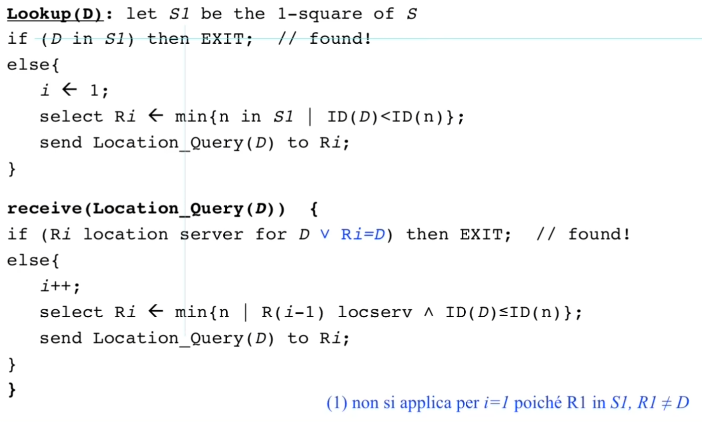
\includegraphics[width=100mm]{img/pseudocoddiffqu.PNG}
\caption{pseudocodice dell'inoltro della query - 1:14 della lezione locsrv2}
\label{fig:pseudo}
\end{figure}
\bigbreak
\noindent \textbf{Lemma 2}: se query da sorgente S a destinazione D, con S e D nello stesso k-quadrato, allora query arriva a D in al più k step.
\bigbreak
\noindent \textbf{Dimostrazione:} \\
Per quanto riguarda k = 1, guardare lemma 1 \\
Per quanto riguarda k $>$ 1: \\
\begin{figure}[h]
\centering
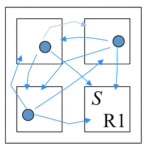
\includegraphics[width=40mm]{img/dimlemma2.PNG}
\caption{dimostrazione}
\label{fig:ferf}
\end{figure}
\bigbreak
\noindent In figura: vediamo un 2-quadrato con i quattro 1-quadrati che lo compongono. Il nodo S deve trovare un nodo D ma non lo vede nel suo 1-quad, S seleziona nel proprio 1-quad il prossimo relay (ID minore tra i maggiori dell'ID di D, R1 è il primo relay). \\ I nodi degli altri 1-quad, dove non c'è la sorgente, devono piazzare un LS in ogni 1-quad in cui non stanno. \\ Consideriamo i nodi \textit{n} negli 1-quad in cui non c'è la sorgente, per cui $ID(D) < ID(n) < ID(R1)$. Se R1 non è LS di D, i nodi che stiamo considerando potrebbero essere dei migliori LS per D rispetto a R1 (hanno un ID maggiore di D ma minore di R1). \\ Se la sorgente sceglie come primo relay R1 è perché R1 è il più piccolo dei più grandi di D in quel 1-quad: nel 1-quad dove c'è la sorgente non esiste altro nodo con ID maggiore di D ma minore di R1. \\ A questo punto, i tre nodi azzurri negli altri 1-quad, quando scelgono il proprio LS devono scegliere il più piccolo dei più grandi di D nell'1-quad in basso a dx, ma è proprio R1 perché non c'è ne è un altro. Questo significa che, all'interno del 2-quad, R1 è LS di tutti i nodi con $ID(D) > ID(n) < ID(R1)$. \\ Questo ci dice che se la destinazione D non ha messo un LS nell'1-quad ma lo ha messo nel 2-quad, allora tutti i nodi che meglio di R1 possono essere LS di D nel 2-quad, stanno in uno dei 1-quad e hanno scelto R1 come LS perché hanno scelto il più piccolo dei più grandi di loro nell'1-quad in basso a dx.

\begin{enumerate}
    \item La sorgente S è nel 1-quad s1 e conosce tutti i nodi all'interno di s1
    \item R1 in s1 è scelto da S in modo che nessun altro nodo \textit{n} in s1 ha $ID(D) < ID(n) < ID(R1)$ (S ha guardato tutti gli n che soddisfano $ID(n) > ID(D)$ e sceglie R1 come il minore tra questi $ID(n) < ID(R1)$).
    \item R1 è LS, nel 2-quad che contiene questo 1-quad, per tutti i nodi \textit{m} che hanno $ID(D) < ID(m) < ID(R1)$ (consideriamo i nodi \textit{m} che stanno nello stesso 2-quad della sorgente, essi hanno un LS in s1 come da criterio nel piazzamento dei LS. Ma il LS di questi nodi \textit{m} è R1 poiché non esiste un nodo \textit{n} in s1 tale che $ID(D) < ID(n) < ID(R1)$).
    \item se non c'è nessun altro nodo intermedio, R1 è LS di D arrivati (D è parte dei nodi \textit{m} che hanno scelto R1 come LS).
    \item altrimenti scegliamo tra i nodi \textit{m}, R2 tale che $ID(D) < ID(R2) < ID(R1)$, cioè R1 sceglie R2 come il più piccolo degli \textit{m} che conosce. 
    \item R2 è LS, nel 3-quad che contiene questo 2-quad, per tutti i nodi \textit{m} che hanno $ID(D) < ID(m) < ID(R2)$. Dopo di che ricomincia lo stesso procedimento. 
\end{enumerate}
Quello sopra è un progressivo avvicinamento nello spazio degli indicatori, $ID(D) < ID(R1)$ poi $ID(D) < ID(R2) < ID(R1)$ e $ID(D) < ID(R3) < ID(R2) < ID(R1)$ etc. Dato che abbiamo assunto che ogni coppia di ID è ordinata e che i veicoli sono in numero finito, se abbiamo l'identificatore di D e mano a mano che scegliamo un nuovo relay ci avviciniamo a quello di D, prima o poi troviamo il LS di D o troviamo direttamente D.  
\bigbreak
\noindent \textit{Se vuoi rivederti la spiegazione della dimostrazione, lezione locsrv3}

\subsection{Efficacia ed efficienza}
\begin{itemize}
    \item [-] Ad ogni step decresce in modo monotono l'id del relay che sto usando
    \item [-] Gli identificatori sono discreti e in numero finito, prima o poi la ricerca si deve fermare, perché arrivo a D
    \item [-] Per le considerazioni precedenti, ad ogni passo salgo di (almeno) 1-ordine di square (in realtà si può dimostrare che si sale esattamente un ordine)
    \item [-] Quando scelgo un $R_x$ nello x-square che contiene D, allora D deve avere scelto $R_x$ come LS perché non c'è altro nodo intermedio migliore
    \item [-] Arrivo a $R_x$ in al più in $x$ passi
\end{itemize}

\subsection{Selezione location server}
\begin{itemize}
    \item [-] location update contiene il quadrato target (quello dove il nodo vuole piazzare un'informazione aggiornata della propria posizione), il location update è inoltrato geograficamente anycast
    \item [-] il primo nodo (RO) incontrato nel quadrato target, mette l'update in una fake query per la destinazione. R0 genera la fake query ed è quindi sorgente.
    \item [-] cerca nel suo 1-quad un nodo R1 migliore di sé, se lo trova gli passa la query con dentro l'update. Se non lo trova il migliore è lui, R0 è location server di D
    \item [-] altrimenti si itera, avvicinandosi ogni volta a ID(D) da sopra
    \item [-] inoltro si ferma quando $R_x$ non conosce nessuno migliore di lui e diventa LS, oppure $R_x$ conosce qualcuno migliore ma fuori dal quadrato target e diventa LS perché i quadrati di ordine inferiore sono già stati scartati
\end{itemize}

\subsection{Strutture dati e messaggi}
\noindent Location table: un nodo deve mantenere una tabella in cui si ricorda tutti gli ID e la posizione dei nodi di cui fa da location server. 
\noindent Location cache: vengono tenute delle informazioni che il nodo origlia, uno step è formato da più di un hop fisico, se nel corso di uno step un nodo intermedio tra due relay, vede passare un messaggio che contiene la posizione di un nodo, è utile che se la ricordi. 

\begin{figure}[h]
\centering
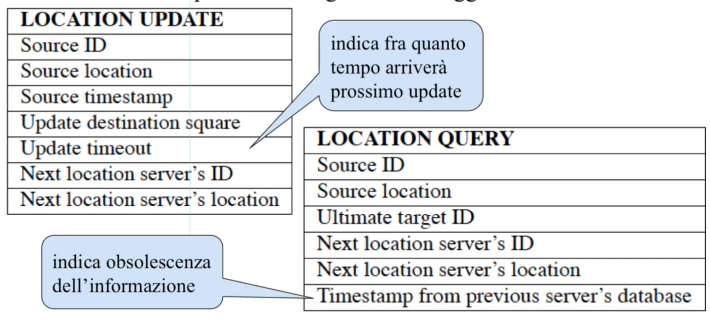
\includegraphics[width=100mm]{img/strdagls.PNG}
\caption{messaggi con parametri}
\label{fig:pseudofefre}
\end{figure}
\noindent In figura, location update: contiene l'id, la posizione e il timestamp (veicoli con GPS) della sorgente, il quadrato di destinazione dell'update, un timeout (indica tra quanto tempo partirà un nuovo update, se questo update non gli arriva può pensare che un altro veicolo, con ID maggiore della sorgente ma più piccolo del suo, sia entrato nel quadrato e quindi sia diventato lui LS), in ultimo ci sono next location server's ID e next location server's location (servono per passare la query da un relay all'altro, cambiando indirizzo e ID del relay destinazione). 
\bigbreak
\noindent In figura, location query: contiene l'ID e la posizione della sorgente (quando la query arriva, la destinazione deve poter rispondere alla sorgente), ultimate target ID (ID della destinazione che stiamo cercando), next location server's ID e next location server's location (come sopra) e timestamp (ci dice quanto è vecchia l'informazione sulla posizione, può servire per raddrizzare la query confrontandola con l'informazione contenuta nella cache). 

\subsection{Gestione mobilità}
\begin{itemize}
    \item [-] se un nodo si muove nello stesso 1-quad non manda update a nessuno 
    \item [-] fissata distanza d, aggiorna i LS in un i-quad quando si sposta di una distanza maggiore $2^{i-2}*d$ dall'update precedente (esponenziale)
    \item [-] l'informazione sulla posizione è messa in piggybacked su ogni pacchetto (permette aggiornamento delle cache)
    \item [-] se non ricevo una risposta, può essere successo che la query sia bloccata in un massimo locale o che ci sia partizione. Viene dato un po' di tempo al nodo per far partire un nuovo update, do' un po di tempo alla rete perché si sistemi la topologia (la prima volta aspetto t, la seconda 2t, la terza 4t - esponenziale). 
    \item [-] quando D si muove tra due 1-quad adiacenti, s1 e s2, potrebbe darsi che non ha ancora aggiornato i suoi LS perché la distanza è molto piccola. Prima di attraversare il confine, faccio partire un messaggio diretto a tutti i nodi del 1-quad (forwarding pointer) di partenza dicendo di inoltrare in s1 i pacchetti diretti a lui. I FP vengono imparati dai nodi che entrano in un 1-quad e dimenticati da chi ne esce. 
\end{itemize}

\subsection{Prestazioni}
GLS con simulazione con fino 600 nodi su un'area 2900x2900m, è stato scelto un raggio radio che è uguale a lato dell'1-quad (250 metri), la densità è circa 100 nodi per $km^2$ cioè circa un nodo per ogni 100x100m. La mobilità è random waypoint.
\bigbreak
Il confronto è stato effettuato con DSR (Dynamic Source Routing, algoritmo per instradamento per mobile ad hoc network, reti più vecchi con meno mobilità, è un algoritmo reattivo che manda in flooding delle route request)
\bigbreak
Con 300 nodi in un'area più piccola garantendo la densità $100/km^2$, la path length della query è poco al di sopra della lunghezza del response path. Le query non fanno cammino molto più lunghi della distanza tra sorgente e destinazione, abbiamo un numero buono di hop, GLS è efficiente. 
\bigbreak
Dopo di che è stato fatto un confronto tra l'instradamento dati di GLS + algoritmo di instradamento geografico e DSR. Con GLS fino alla massima espansione dell'area (2900x2900) circa il 90\% dei dati è consegnato, DSR cala subito dopo i 300 nodi (dipende dall'alto carico imposto sulla rete dal flooding).


\chapter{Inoltro geografico}
Bibliografia - si trovano in lezione e materiali didattici: 
\begin{itemize}
    \item[-]S.Giordano, I.Stojmenovic, L.Blazevic 
    \textit{Position-based routing algo for ad hoc networks:a taxonomy - fino a pagina 9 incluse}
    \item[-] B.Karp, H.T.Kung
    \textit{GPSR: Greedy Perimeter Stateless Routing for Wireless Networks}
\end{itemize}

\section{Position Based Routing}
Siamo sempre in una rete con alta mobilità e velocità alte (considerando le velocità relative tra veicoli), non ha molto senso imparare la topologia della rete in un dato momento. Dobbiamo trovare un metodo per far arrivare un pacchetto da un nodo sorgente S ad una destinazione D, conoscendone la posizione. 
\bigbreak
In generale: quando un nodo riceve un pacchetto rivolto a lui, guarda se la destinazione è nei propri vicini. Nel caso non fosse fa un tentativo di inoltro a nodi che sono più vicini alla destinazione.
\bigbreak
\noindent Assunzioni:
\begin{itemize}
    \item i nodi devono conoscere la propria posizione (GPS)
    \item i nodi devono conoscere la posizione dei vicini (beacon, HELLO message)
    \item i nodi devono conoscere la posizione della destinazione (location service)
\end{itemize}
\bigbreak
\noindent Numerose politiche proposte in letteratura:
\begin{itemize}
    \item [-] flooding direzionale: una delle prime soluzioni pensate quando la mobilità è molta alta. Il LS ci da la posizione della destinazione e viene fatto un flooding ma direzionato (a un insieme $k$ di vicini) che permette di avvicinarsi alla destinazione. \\ Il fatto che ci siano più copie di pacchetto, una per ogni $k$ vicino, offre robustezza (se un cammino si rompe, ne ho altri) \\ Può funzionare bene per il geocasting, trovare nodi in una determinata area. \\ In generale è un approccio con alto costo. 
    \item [-] unicast a vicino appropriato (on-demand): sono il tipo di soluzioni che affrontiamo in questo corso
\end{itemize}

\subsection{Indici di prestazione}
Di cosa mi preoccupo e cosa devo tener presente quando progetto algoritmo:
\begin{itemize}
    \item [-] i cammini non devono avere loop (mi occupano canale), consegna garantita (modalità promiscua dei nodi che possono origliare se un messaggio è stato inoltrato), scalabilità, robustezza ai fallimenti (in una rete wireless, fragile è molto utile)
    \item [-] operazioni distribuite (più la rete è distribuita meglio è), stateful o stateless (guadagno in scalabilità se non mantengo informazioni di stato, meglio stateless)
    \item [-] strategia da usare per creare path (single path, c'è una sola copia di pacchetto che passa da un nodo all'altro. Flooding prevede di mandare una copia a tutti i nodi, multi-path è una via di mezzo)
    \item [-] metrica usata (meno hop possibili, metodo che risparmia più energia possibile, metodo che risparmia in costo oppure in qualità)
    \item [-] requisiti fisici (caratteristiche delle tecnologie radio dei veicoli o dei sensori - ad ex. avere GPS), requisiti aggiuntivi di sistema (devono conoscere una mappa condivisa)
    \item [-] quanto spesso abbiamo bisogno di aggiornare la posizione dei nodi (dipende dalla mobilità), QoS (dobbiamo vedere se abbiamo vincoli di qualità, dati di safety devono arrivare con bassa latenza ad ex), problematiche di congestione e scheduling delle attività dei nodi (de-sincronizzare i nodi mi aiuta a non creare interferenze tra i segnali).
\end{itemize}

\section{Politiche greedy}
Sono euristiche, non ci garantiscono niente, fanno del loro meglio per consegnare i pacchetti. Molte politiche greedy sono basate sull'idea di \textbf{progresso}.
\bigbreak
\noindent Progresso: il nodo S ha in mano un pacchetto da inoltrare, S ha un determinato raggio radio rappresentato dal cerchio. Tracciamo il segmento che unisce S e D, dopo di che proiettiamo A sul segmento. La perpendicolare individua un punto A' sul segmento SD, il progresso di A è la lunghezza del segmento A'D. 
\begin{figure}[h]
\centering
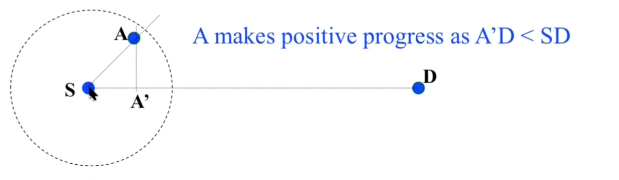
\includegraphics[width=90mm]{img/progress.PNG}
\caption{rappresentazione del progresso}
\label{fig:pseuopefre}
\end{figure}
\bigbreak
Il vicino A ha progresso positivo: devo guardare le distanza, sulla direttrice, dei nodi considerati dalla destinazione. Guardo SD e A'D, il progresso è positivo se A'D $<$ SD (l'attuale nodo trasmittente è 1000m da D, A' dista 700m da D, allora il progresso è positivo). Se poniamo di avere un nodo B dall'altra parte rispetto ad A, proietto e ottengo B'D, in questo B'D $>$ SD per cui il progresso sarebbe negativo. 
\bigbreak
L'idea  di molte strategie greedy è di scegliere uno dei vicini che ha un progresso positivo, non necessariamente quello con il progresso maggiore. 

\subsection{Selezione greedy dei vicini}
\begin{itemize}
    \item [-] \textbf{RPM} (Random Progress Method): guarda tutti i vicini con progresso positivo, se sono più di uno, ne sceglie uno a caso.
    \bigbreak
    La componente randomica è utile perché risolve il problema di aver scelto una volta un nodo che ha perso il pacchetto, la volta successiva ne viene scelto un altro sicuramente. La randomness mi aiuta anche per difendermi da attaccanti malevoli.
    \item [-] \textbf{MFR} (Most Forward within Radius): tra tutti i vicini con progresso positivo, sceglie quello con il maggior progresso. Possiamo anche dire che è quello che minimizza la distanza tra la proiezione e la destinazione (se ci fosse un punto C' tra S e A' allora $SD > C'D > A'D$, sceglierebbe A perché ha la minore distanza tra A' e la destinazione). 
    \bigbreak
    Compie salti lunghi e meno frequenti, i ritardi si accumulano hop per hop per questo MFR riduce la latenza. MFR tende a far parlare nodi distanti, potrebbe darsi che tra questi nodi ci siano molti altri nodi in mezzo e creo collisione. 
    \item [-] \textbf{NFP} (Nearest with Forward Progress): tra i vicini con progresso positivo, viene scelto il nodo con distanza minore dal nodo trasmittente (guarda se SA $<$ SB o se SA $<$ SC). 
    \bigbreak
    Parlano nodi molto vicini, tendo a fare hop corti e frequenti (parlo con bassa potenza, minore probabilità di collisione ma latenza più alta). 
    \item [-] \textbf{Greedy scheme}: prende il vicino con la minima distanza dalla destinazione, indipendentemente dalle proiezioni.
    \item [-] \textbf{DIR} (Compass Routing): sceglie il vicino del nodo corrente tale che la direzione nodo corrente-vicino è la più vicina alla direzione nodo corrente-destinazione. Compasso è perché si guardano gli angoli tra le direzioni, vorrei lo scostamento d'angolo minore. 
    \bigbreak
    Il lato positivo è che ci perdiamo meno, andiamo quasi sempre in direzione della destinazione. Il compass routing però incorre spesso i cammini con loop che non arrivano alla destinazione.
\end{itemize}

\subsection{Problemi approcci greedy}
Abbiamo la sorgente S del messaggio, S ha capito dal location service le coordinate della destinazione D, S usa una delle politiche greedy spiegate sopra. 
\begin{figure}[h]
\centering
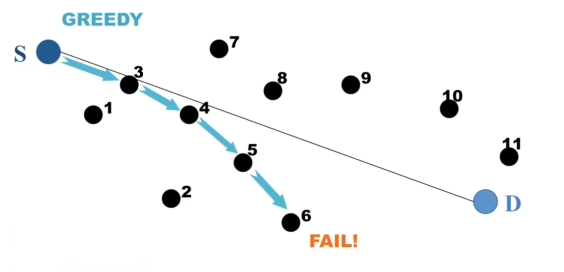
\includegraphics[width=90mm]{img/probgreed.PNG}
\caption{problema di massimo locale}
\label{fig:ferger}
\end{figure}

\noindent In figura: il nodo 6 è quello che ha raggiunto la distanza minima da D, siamo in un punto cieco e il nodo 6 butta via il messaggio (approccio store and forward). \\ Questa situazione si verifica con tutte le politiche greedy spiegate sopra. 
\bigbreak
La soluzione è trovare una strada alternativa per aggirare l'ostacolo: posso tornare indietro fino al nodo 4, il nodo 4 sceglie una strada alternativa che passa per il nodo 8, 9, 10, 11 e arriva D. Quest'altra strada magari è più lunga e va in una direzione lontana rispetto alla destinazione, ma alla fine ci permette di raggiungere la destinazione. 

\subsection{Strategie di recupero - euristiche}
Posso applicarle a qualsiasi delle politiche greedy sopra dette.
\begin{itemize}
    \item [-] \textbf{Flooding}: sono in un massimo locale, il nodo replica il pacchetto a tutti i suoi vicini (nell'ex. il nodo 6 manda il pacchetto a tutti i suoi vicini). I vicini se possono scegliere un vicino buono rispetto a una politica greedy, inoltrano al vicino buono, se il vicino buono è quello che gli ha mandato il pacchetto in flooding, il vicino fa flooding a sua volta.
    \bigbreak
    Non ho più il controllo del flooding, molte copie in giro, collisioni e uso di banda massiccio
    \item [-] \textbf{Alternate}: il vicino nel massimo locale inoltra il pacchetto ai $k$ vicini meno peggio (ad ex. un nodo con progresso negativo ma non eccessivamente grande). 
    \item [-] \textbf{Disjoint}: il nodo ha inoltrato ad un vicino, il vicino gli ha rispedito il pacchetto, allora il nodo inoltra ad un suo vicino diverso (alternate manda in parallelo a $k$ vicini, disjoint manda sequenzialmente).
\end{itemize}

\subsection{Strategie di recupero - GPSR}
Strategia formalmente più solida, si basa su teoria dei grafi. 

\section{GPSR (Greedy Perimeter Stateless Routing)}
La rete è stateless (non vengono tenute informazioni di stato sulla topologia intera della rete), ho informazioni sul mio vicinato e ci ragiono un po' meglio. \\ Fino a che va tutto bene è usata una delle politiche greedy, nel momento in cui la politica greedy mi porta in un massimo locale uso un meccanismo di recovery. \\ Devo trovare il modo per superare l'area vuota intorno al massimo locale, GPSR cerca di capire di più sul vicinato dei nodi e cerca un modo per percorre il perimetro dell'area vuota per aggirarla. 
\bigbreak
\noindent GPRS garantisce di: 
\begin{itemize}
    \item [-] trovare un percorso sul perimetro dell'area vuota per poterla aggirare
    \item [-] altrimenti di trovare un loop e fare in modo che il messaggio torni indietro su questo percorso. Questo tornare indietro segnala ai nodi che il cammino sicuramente non c'è, se no GPRS l'avrebbe trovato (il pacchetto viene buttato perché la rete è partizionata e non c'è modo di consegnarlo). 
\end{itemize}
\noindent Assunzioni GPRS:
\begin{itemize}
    \item [-] link bidirezionali e presenza location service
    \item [-] beacon periodici tra vicini con ID e posizione (ogni nodo mantiene una tabella dei vicini, informazioni di stato locali)
    \item [-] ogni pacchetto carica sia la posizione della destinazione sia la posizione corrente del mittente (il destinatario può rispondere alla sorgente e i nodi intermedi possono sniffare la posizione della sorgente e metterla in cache). 
    \item [-] le schede di rete dei nodi sono in modo promiscuo (possono origliare pacchetti non diretti a loro)
 \end{itemize}
 
La politica di recovery potrebbe venir usata fin dall'inizio, ma richiede un po' più di calcolo ai nodi e non garantiscono di trovare il cammino più breve (posso farlo se voglio forti garanzie sul fatto che il pacchetto arrivi a destinazione, non mi interessa che percorra un cammino più lungo, basta che arrivi alla destinazione o che mi venga notificato il contrario)
 
\subsection{Funzionamento}
\begin{figure}[h]
\centering
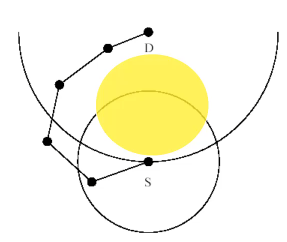
\includegraphics[width=40mm]{img/gpsr.PNG}
\caption{GPSR esempio}
\label{fig:fergerfrr}
\end{figure}
\noindent In figura: c'è un nodo trasmittente S che deve inoltrare un pacchetto. Il nodo S è arrivato al massimo avvicinamento possibile rispetto alla destinazione (l'unico vicino che ha nel suo raggio radio è più lontano dalla destinazione).
\bigbreak
Le strategie di recupero euristiche generano copie difficili da controllare, cerchiamo di mantenere un approccio unicast che permetta di trovare un path che aggira l'area vuota gialla. 
 \begin{figure}[h]
\centering
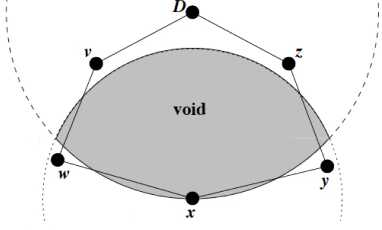
\includegraphics[width=60mm]{img/gpsr2.PNG}
\caption{GPSR teoria dei grafi}
\label{fig:fergerfrffr}
\end{figure}
\bigbreak
\noindent In figura: il nodo $x$ ha il pacchetto diretto alla destinazione D. 
\bigbreak
\noindent L'idea è di definire dei poligoni, aperti o chiusi, percorrendone tutti i lati arriviamo alla destinazione e se continuiamo torniamo alla sorgente $x$. Anche se il poligono è visivamente aperto, essendo i link bidirezionali è come se il poligono fosse chiuso. 
\bigbreak
\noindent \textbf{Face}: regione poligonale chiusa tra archi
\bigbreak
\noindent \textbf{Regola mano destra}: nei labirinti esiste una regola di percorrenza che consiste nell'appoggiare una mano ad un muro e tenerla sempre così mentre ci si muove. Nella teoria dei grafi, la regola della mano dx, garantisce di tornare al punto iniziale in cui si è appoggiata la mano sul muro (non è garantito di arrivare al centro, di percorrere la strada più corta né di percorrere tutti i path disponibili). 
\bigbreak
Arrivo in un punto del mio grafo da un arco (percorro arco \textit{yx} e mi trovo in x), guardo chi è il path ancora non percorso più vicino in senso antiorario, trovo \textit{xw} e lo percorro arrivando in w. Guardo chi è il path più vicino in senso antiorario e trovo \textit{wv} e lo percorro e così via.
In questo modo percorro tutta la face, se non trovo il nodo destinazione ad un certo punto mi ritroverò nel nodo iniziale (capendo che sono in loop) mentre se trovo la destinazione, blocco il tour e consegno il pacchetto. 
\bigbreak
GPSR funziona con qualsiasi politica greedy come strategia di instradamento di base. In presenza di massimo locale si entra in modalità perimetro, in figura entriamo in modalità perimetro nel nodo \textit{x}.
\begin{figure}[h]
\centering
\includegraphics[width=50mm]{img/gpsr3.PNG}
\caption{GPSR come funziona}
\label{fig:gpsrmodper}
\end{figure}
\newpage
\begin{itemize}
    \item [-] il pacchetto entra in modalità perimetro in \textit{x} (nell'header è marcato come perimeter mode).
    \item [-] il nodo \textit{x} segna le sue coordinate nel pacchetto, utili perché tutti i nodi devono sapere calcolare il segmento \textit{xD}.
    \item [-] il nodo \textit{x} costruisce il grafo planare proprio e dei suoi vicini 
    \item [-] considera la direttrice \textit{xD} e si muove in senso antiorario prendendo il primo arco che incontra e inoltra il pacchetto a quel vicino (regola della mano destra dove il muro è la direttrice).
    \item [-] il vicino scelto si vede arrivare un pacchetto: vede che GPRS è in perimeter mode, vede che deve arrivare alla destinazione D e vede le coordinate del nodo \textit{x}.
    \item [-] il vicino controlla se è possibile passare in greedy mode, se è così inoltra il pacchetto al suo vicino "migliore"
    \item [-] se non è possibile passare in greedy mode continua in perimeter.
    \item [-] il vicino crea il suo grafo planare, successivamente deve "trovare" la direttrice: procedendo in senso anti-orario, vede se ha un arco con un suo vicino che attraversa la direttrice oppure, se così non fosse, proietta sé stesso sulla direttrice. A questo punto gira in senso anti-orario fino a trovare l'arco da percorre.
\end{itemize}
E' possibile dimostrare che la regola della mano destra in un grafo planare trova un cammino fino alla destinazione, se un cammino esiste. 

\subsection{Grafi planari}
Abbiamo quindi la questione di determinare le faces. Per fare questo devo eliminare gli archi che si incrociano, determinando un \textbf{grafo planare}, cioè un grafo in cui ogni coppia di archi non si incrocia. Questo va fatto con attenzione, è come dire ad alcuni nodi che non devono sentire alcuni loro vicini, ma vuol dire anche potare la possibilità di due nodi di sentirsi, magari creando anche partizioni se lo faccio male. Il grafo planare è ottenuto attraverso computazione locale di ciascun nodo, cancello archi senza disconnettere nodi, inoltro va ricalcolato ad ogni cambio di vicinato (parte onerosa di GPRS)
\bigbreak
\noindent \textbf{Relative Neighborhood Graph}
\begin{figure}[h]
\centering
\includegraphics[width=30mm]{img/RNG.PNG}
\caption{RNG}
\label{fig:fffeg}
\end{figure}
\bigbreak
\noindent In figura: poniamo che ci sia un arco tra il nodo \textit{u} ed il nodo \textit{v}. Traccio un cerchio con centro in \textit{u} e raggio pari alla distanza tra \textit{u} e \textit{v} e faccio la stessa usando come centro il nodo \textit{v}. Osserviamo se all'interno della lunetta di intersezione tra le due circonferenze ci sia un altro nodo, se c'è un nodo (ad ex. \textit{w}) posso eliminare l'arco \textit{uv}. Posso dirlo anche così: se $d(u,v) <= max[d(u,w), d(v,w)]$ allora non elimino l'arco \textit{u,v}.
\bigbreak
\noindent \textbf{Gabriel graph}
\begin{figure}[h]
\centering
\includegraphics[width=30mm]{img/gabriel.PNG}
\caption{Gabriel graph}
\label{fig:ffbeg}
\end{figure}
\bigbreak
\noindent In figura: poniamo che ci sia un arco tra il nodo \textit{u} ed il nodo \textit{v}. Traccio le due circonferenze allo stesso modo di Relative Neighborhood Graph, traccio anche la circonferenza ombreggiata. Per disegnare quest'ultima, considero come centro della circonferenza il punto medio \textit{m} dell'arco \textit{uv} e il raggio come la distanza \textit{mv}. Considero l'area ombreggiata, se ho un altro nodo \textit{w} all'interno allora possiamo eliminare l'arco \textit{uv}. \\
RNG elimina più archi rispetto a gabriel graph. 

\subsection{Prestazioni}
Valutate in simulatore, con 802.11p con radio range di 250m, mobilità scelta è random waypoint, confrontiamo con DSR (Dynamic Source Routing per MANET). DSR arriva a circa 97\% di pacchetti consegnati, mentre GPRS ha valori più alti. Abbiamo alta affidabilità, alta garanzia di consegna dei pacchetti.  

\chapter{Internet of things}
Bibliografia - si trovano in lezione e materiali didattici: 
\begin{itemize}
    \item[-] L.Atzori, A.Iera, G.Morabito 
    \textit{The internet of Things: a survey - pp.2787-2805}
\end{itemize}
"A world-wide network of interconnected objects uniquely addressable, based on standard communication protocols". 
\bigbreak
Il mondo IoT è visto come diviso in tre piani: semantic-oriented (tecnologie per ragionare sfruttando la grande mole di dati generata), things-oriented (molto piccoli e pervasivi) e Internet-oriented (parte di comunicazione).
\bigbreak
\section{LLNs (Low-power Lossy Networks)}
Siamo in un contesto di reti fragili, wireless che potrebbero portare a perdere pacchetti e a spezzare link tra nodi. Devo riuscire a mettere in comunicazione queste reti con l'Internet. Gli oggetti usati in queste reti sono device integrati su altri oggetti quotidiani (cyber-physical systems), sono device con potenza, memoria e risorse limitate. 
\bigbreak
C'è differenza tra full function (device di rete che implementano per intero lo stack di protocolli IPv6 e magari hanno anche interfacce verso oggetti non full function) e reduce function (oggetti molto semplici, con risorse limitate che non riescono a implementare tutto lo stack). Dobbiamo responsabilizzare i full function device perché aiutino device più limitati. Non tutti i nodi hanno lo stesso ruolo, un po' alla three-tier architecture. 
\bigbreak
Gli smart object hanno un minimo insieme di funzioni di comunicazione, possiedono un identificatore univoco (se sono full function IPv6) e un nome. Il nome deve anche fornire una descrizione human-readble che indica le funzioni, non cerco tanto l'ID ma piuttosto il servizio (publish-subscribe). 
\bigbreak
\noindent \textbf{Eterogeneità}: device eterogenei, per cui si punta molto sul voler standardizzare in modo da offrire interoperabilità
\bigbreak 
\noindent \textbf{Ricerca e composizione}: non è detto che tutti gli standard siano implementati da tutti gli oggetti, oggetti diversi implementeranno parti diversi di standard a secondo delle loro possibilità. Dovrò fare composizione di servizi e funzionalità differenti.
\bigbreak
\noindent \textbf{Machine to Machine (M2M)}: si elimina la parte umana, comunicano solo le macchine
\bigbreak
Tutto ciò richiede nuove soluzioni a livello di network (6TiSCH) e applicazione (MQTT). Richiede ovviamente scalabilità su milione di nodi.
\bigbreak
\noindent \textbf{Industry 4.0}: parte di IoT con requisiti particolari. Tutti gli oggetti sono connessi attraverso IoT o IoP, sono oggetti autonomi (operano senza ausilio umano), voglio che siano deterministici e con bassa latenza, ma voglio anche molta affidabilità. Solitamente ci troviamo in ambienti difficili (calore, umidità, sabbia, interferenza), in più in comune all'IoT devono offrire scalabilità, resistenza ai fallimenti, eterogeneità dei device. 

\chapter{6TiSCH}
\section{Concetti base}

\subsection{CSMA/CA}
CSMA/CD è lo standard di accesso al canale usato da Ethernet, Ethernet è uno standard per reti cablate. Collision Detection perché le schede di rete stanno in ascolto del canale, mentre trasmettono, per capire se c'è stata interferenza. CSMA/CA è un protocollo di accesso multiplo che utilizza il rilevamento della portante ma in cui i nodi tentano di evitare a priori il verificarsi di collisioni. Una volta iniziata, la trasmissione prosegue fino al termine del pacchetto (viene spesso usato in reti senza fili). Questo perché nelle tecnologie wireless è impossibile fare collision detection, queste schede di rete non posso ascoltare il canale mentre trasmettono (potrebbero ma costerebbero molto).
\bigbreak
\noindent CSMA/CA:
\begin{itemize}
    \item [-] CS (Carrier Sense): prima di trasmettere ascolto il canale per capire com'è la situazione, se lo vedo occupato aspetto un tempo casuale, se nessuno sta trasmettendo, ci provo io
    \item [-] MA (Multiple Access): a uno stesso canale possono accedere contemporaneamente più stazioni
    \item [-] CA (Collision Avoidance)
\end{itemize}

\noindent CSMA/CA funziona così: la stazione fa sensing, ascolta il canale per un po' di tempo, se è libera, sta in ascolto ancora per un piccolo range di tempo (DIFS). Terminato DIFS fa di nuovo sensing del canale, se il secondo sensing dice che il canale è libero, manda il frame. Se il primo o il secondo sensing dicono che il canale è occupato, la stazione ricorre alla procedura di bakeoff (aspetta un tempo casuale per de-sincronizzare). 

\subsection{Slotted Aloha}
Protocollo che prevede di trasmettere quando si vuole trasmettere, se ci riesci bene se no prima o poi riproverai. Le stazioni sono \textbf{sincronizzate} (orologi sincronizzati - tutte le stazioni sono d'accordo su quando inizia uno slot) e il passare del tempo è suddiviso in slot temporali, ogni slot è lungo abbastanza per l'invio di un frame di livello 2. Una stazione può mandare solo all'inizio del time slot, se il frame non è pronto all'inizio di uno slot, la stazione mette il frame nel buffer perché non può trasmettere a metà slot. Se due stazioni scelgono due slot diversi per trasmettere, non ci saranno sovrapposizioni. 

\subsection{Time Division Multiplexing}
Tecnica di accesso deterministico al canale.
\begin{figure}[h]
\centering
\includegraphics[width=40mm]{img/TDA.PNG}
\caption{Time Division Multiple Access}
\label{fig:tda}
\end{figure}
Suppongo di avere 4 stazioni (discriminate per colori in figura), assegno ad ognuna di loro un quanto di tempo abbastanza lungo per trasmettere un frame. Adotto una politica Round Robin dicendo che nel primo slot parla la lilla, nel secondo la gialla, nella terza la verda, nel quarto la blu e nella quinta la lilla e via così ricominciando. Abbiamo una grande equità di suddivisione del canale tra le varie stazioni. Nel momento in cui una stazione trasmette usa l'intero spettro di frequenze utilizzabili, tutta la banda trasmissiva a disposizione. 

\subsection{Frequency Division Multiplexing}
Tecnica di accesso deterministico al canale.
\begin{figure}[h]
\centering
\includegraphics[width=40mm]{img/FDM.PNG}
\caption{Frequency Division Multiple Access}
\label{fig:fdma}
\end{figure}
Ciascuna stazione può trasmettere per tutto il tempo che vuole, ma solo su $1/n$ (con n stazioni connesse alla rete) delle frequenze disponibili sul canale. Nel primo quarto di frequenza disponibili trasmette la stazione blu, nel secondo quarto parla la verde, nel terzo la gialla e nel quarto la lilla. Non c'è collisione, parlano nello stesso tempo ma usano frequenze diverse.  
\bigbreak
Sono entrambe deterministiche perché sappiamo chi accede al canale. Garantiscono bassa latenza, non ci sono tempi di bakeoff, quando una stazione deve mandare qualcosa ha uno slot di tempo o uno spettro di frequenza assegnata. Garantiscono alta affidabilità, eliminiamo qualsiasi interferenza tra stazioni. 
\bigbreak
Sono tecnologie un po' vecchie e sono state un po' abbandonate:
\begin{itemize}
    \item [-] TDM: se una stazione non ha nulla da mandare, lo slot di tempo assegnatole va perso perché nessun' altro può trasmetterci sopra.
    \item [-] FDM: se una stazione non ha nulla da mandare, il suo spettro di frequenza rimane inutilizzato e non è riassegnato a stazione che ne avrebbero bisogno
\end{itemize}
\noindent \textbf{FDM + channel hopping}: due stazioni S e D si parlano, la stazione S,ogni volta che manda un frame, usa un sotto-intervallo diverso di frequenza rispetto alla volta precedente. Per fare questo segue uno schema di salto pseudo-casuale (all'inizio della conversazione tra S e D è stato negoziato, si sono accordate le due stazioni). Supponendo di star usando un canale wireless, quindi prono ad errori e interferenze di sorgenti esterne (microonde, motori industriali) su certe frequenze, se S parla proprio a questo frequenze, i suoi dati possono essere distrutti. La mia sorgente deve ritrasmettere, ma facendo channel hopping, il sotto-intervallo di frequenze con il quale trasmette cambierà, evitando collisioni (aumento robustezza). Questo mi risolve anche il problema di assegnare un sotto-intervallo ad una sola stazione (e se a lei non serve, va perso). Le stazioni usano spettri di frequenze diverse e li slottizzano a tempo (prendo un po' di TDM). 

\section{6TiSCH}
Architettura con riferimento a IPv6 per la comunicazione di apparati wireless con memoria, potenza e batteria ridotta. 
\begin{figure}[h]
\centering
\includegraphics[width=40mm]{img/boh.PNG}
\caption{Confronto tra stack IoT e stack standard WSN}
\label{fig:oode}
\end{figure}
Partendo dal basso dello stack:
\begin{itemize}
    \item [-] a livello fisico usiamo lo standard 802.15.4 (working group dedito alle WSN). In generale 802.15 si occupa di Wireless Specialty Networks. 
    \item [-] a livello MAC: prima veniva usata CSMA/CA, adesso viene usato 802.15.4e (TSCH) che è fatto apposta per essere efficiente in latenza e affidabilità. TSCH è protocollo standard di livello MAC dell'architettura 6TiSCH (è qui che avviene frequency e time division e channel hopping)
    \item [-] a livello Logical Link Control: uso 6top che da direttive a TSCH su come accedere al canale
    \item [-] 6LoWPAN HC: middleware che ha il compito di tradurre i pacchetti di formato IPv6 (di grandi dimensioni) per farli stare nei frame di livello inferiore (TSCH) che devono invece essere piccoli perché la banda è ridotta. Ci saranno dei gateway che permettono l'accesso alla rete IoT anche a dispositivi, pacchetti che non usano lo stack 6TiSCH. 
    \item[-] RPL: protocollo di instradamento per standard IoT. Esistono due varianti in accordo alla distinzione full function e reduce function. 
    
\end{itemize}

\section{6TiSCH network structure}
\begin{figure}[h]
\centering
\includegraphics[width=60mm]{img/tschns.PNG}
\caption{Struttura di rete}
\label{fig:oodfffe}
\end{figure}
C'è Internet, classica vecchia rete cablata indirizzata con IPv6, abbiamo una backbone cablata in modo standard. Abbiamo poi dei backbone router (6LBR) che fungono da interfaccia tra Internet cablato e le LLN (Low power Lossy Network), dove 6 sta per 6TiSCH, L per LLN e BR per Border Router. 
\bigbreak
Questi 6LBR possono costruire anche delle LLN federate, le due LLN vogliono costituirsi per rappresentare un'unica LLN (anche se non hanno esattamente gli stessi protocolli), 6LBR deve fungere da intermediario per farle funzionare come un'unica rete LLN. 
\bigbreak
\noindent 6LBR funzioni:
\begin{itemize}
    \item [-] c'è un'idea di slot di temporale: fanno da time source neightbors, cioè danno un orario comune ai nodi. 
    \item [-] sono root dei cammini RPL, protocollo di instradamento
    \item [-] sono entità centralizzate che implementeranno il protocollo 6top che controlla qual è il funzionamento della rete e le richieste delle applicazioni e, in base a questo, da indicazioni su come accedere al canale. 
    \item [-] intermediario tra Internet IPv6 e LLNs
\end{itemize}
Le LLN sono viste come mesh network (non molta mobilità), sono viste come reti multi-hop.

\section{TSCH - Time Slotted Channel Hopping}
Supporta comunicazione LLN anche con possibilità di soddisfare requisiti di qualità (industry 4.0). 
\begin{figure}[h]
\centering
\includegraphics[width=70mm]{img/tsch.PNG}
\caption{Sfruttamento del canale}
\label{fig:tschcanale}
\end{figure}
\noindent In figura: sulle ascisse ho la rappresentazione di TDM e sulle ordinate di FDM. Sulle ascisse ho 0, 1, 2, 3 e poi di nuovo 0 (in accordo a Round Robin per TDM), viene stabilito un numero massimo di time slot per ogni frequenza e poi ricomincio.
\bigbreak
TSCH lavora sopra 802.15.4 e quindi in una banda intorno al 2.4GHz divisa in 16 sottocanali. TSCH utilizza TDM e FDM, il secondo lo usiamo nella variante con channel hopping.  TSCH usa anche il meccanismo di Slotted Aloha per cui un frame deve aspettare l'inizio di uno slot per essere trasmesso. 
\bigbreak
Per fare TDM gli orologi devono essere sincronizzati, posso sincronizzare usando i 6LBR (essendo connessi alla rete Internet, possono chiedere ai server NTP).
\bigbreak
Stazioni che parlano in frequenze diverse, possono parlare contemporaneamente, nello stesso canale dobbiamo impedire le collisioni. Ci sono due tipi di time slot, rossi e blu:
\begin{itemize}
    \item [-] time slot rossi - shared:  possono essere acceduti da chiunque stia trasmettendo/ricevendo su quel sotto-canale, sono slot a contesa, la stazione che accede manda il suo frame all'inizio del time slot shared secondo CSMA/CA.
    \item [-] time slot blu - viene specificata la coppia di nodi che può parlare (sorgente-destinazione): c'è anche specificato un tempo di risposta per permettere alla destinazione di mandare un ACK. Se la destinazione deve mandare dei dati veri e propri dovrà utilizzare un altro time slot. 
    \item [-] time slot bianchi: non sono assegnati e nessuno può parlare
\end{itemize}
Dal punto di vista energetico, in uno slot shared qualunque stazione è sintonizzata su quel canale dev'essere accesa (chi trasmette ovviamente, chi non ha niente da mandare sta acceso perché potrebbe essere la destinazione del messaggio). Le celle shared sono potenzialmente un gran consumo di energia. \\ Nelle celle blu dedicate, le stazioni sanno che nella sotto-frequenza $x$ nel time slot $y$ è la stazione A che manda B, tutte le altre stazioni, che non sono A e B, e che sono sintonizzate su quel canale possono restare spente. Le celle dedicate danno affidabilità (impedendo interferenze), non abbiamo ritardi (non c'è contesa sul canale) e si risparmiano batterie. 

\subsection{struttura dei canali}
La figura sopra mostra una matrice di suddivisione in tempo e frequenze chiamata Channel Distribution and Usage (CDU). Questa viene calcolata da 6hop, protocollo nel livello Logic Link Control e calcolata dai 6LBR. 
\begin{itemize}
    \item [-] I time slot devono permettere la trasmissione di un frame di dimensione massima + trasmissione di un piccolo ACK. 
    \item [-] I time slot sono raggruppati in una slot frame (numero di slot prima che inizino a ripetersi). La lunghezza dello slot frame dipende da qualcosa che viene calcolato da 6hop.
    \item [-] Nodi sono sincronizzati: sanno quando inizia lo slot 0, sanno quanto è lungo lo slot frame e conoscono l'inizio di ogni time slot.
    \item [-] La sincronizzazione è fatto così: il timestamp è messo in piggybacked su qualsiasi pacchetto, sia frame che ACK, questo consente di mantenere la sincronizzazione, anche per device reduce function. Se non c'è scambio dati, 6LBR manda un messaggio per aggiornare e sincronizzare la rete. 
    \item [-] \textbf{Bundle}: individua un canale virtuale tra due stazioni, in ciascuno slot passo $x$ bps, il bundle è composta da $2x$ (gli slot di un bundle possono trovarsi anche in sotto-frequenze diverse). \\ Insieme di celle dedicate (blu) tra A e B in modalità full-duplex. 
\end{itemize}

\subsection{Timeslot}
\begin{figure}[h]
\centering
\includegraphics[width=70mm]{img/timeslot.PNG}
\caption{Composizione dei timeslot}
\label{fig:frefe}
\end{figure}

\noindent In figura sopra:
\begin{itemize}
    \item [-] CCA è il periodo in cui le radio si sintonizzano sul canale (ascoltano il canale e vedono se è utilizzabile). 
    \item [-] In T2 viene mandato il messaggio
    \item [-] Alla fine della trasmissione (prima di T3, nel rettangolo bianco) avviene la commutazione da trasmittente a ricevente per ricevere ACK.
    \item [-] La stazione aspetta per un po' di tempo finché non vede arrivare l'ACK. 
\end{itemize}

\noindent In figura sotto:
\begin{itemize}
    \item [-] TsRrOffset: un periodo è lasciato perché si sintonizzi sul canale e si prepari alla ricezione 
    \item [-] PWT: viene dato un range di sicurezza per l'ascolto, potrebbe esserci una leggera de-sincronizzazione degli orologi. 
    \item [-] In T2 la stazione inizia la ricezione del pacchetto.
    \item [-] Alla fine della ricezione del pacchetto, nel rettangolo bianco, c'è commutazione di radio, si resta sulla stessa frequenza, ma ora questa stazione è in modalità trasmissione per mandare l'ACK.
\end{itemize}
Questo funziona con comunicazione unicast, se abbiamo un time slot blu dedicato per comunicazione broadcast, gli ACK non sono mandati se no il mittente dovrebbe riceverne troppi. Le comunicazione broadcast non sono affidabili in TSCH. 

\subsection{Problemi nell'assegnamento dei time slot - non c'è in esame}
La CDU dev'essere costruita in modo che sfrutti bene la FDM e deve tener presente anche il problema delle hidden station. Diventa un problema di colorazione dei grafi:
\begin{itemize}
    \item [-] due nodi vicini non possono trasmettere sullo stesso time slot sulla stessa frequenza 
    \item [-] due nodi con un vicino in comune non possono trasmette nello stesso time slot sulla stessa frequenza (nel disegno il nodo 1 e 2 sentono sia 0 e 3, se questi ultimi due nodi parlano nello stesso slot sulle stesse frequenze, si crea interferenza)
    \item [-] due nodi lontani, senza vicini in comune possono parlare sullo stesso time slot sulla stessa frequenza (nella colorazione del grafo, hanno lo stesso colore)
    \item [-] minimizzare il numero di colori massimizza il numero di frequenze. Se massimizziamo le frequenze possiamo massimizzare l'uso del canale (moltiplico la stessa frequenza per tutti i nodi dello stesso colore che le utilizzano, molti nodi in parallelo usano la stessa sotto-banda) 
    \item [-] lo scheduling dei time slot e l'organizzazione degli slot frame dipende anche dall'applicativo e da come sono collegati i nodi. E' molto difficile ottimizzarlo per tutti i cammini nel grafo. 
\end{itemize}

\subsection{Channel hopping}
 Da uno slot frame all'altro si rifà la mappatura dei sotto-canali sui canali reali di sotto-frequenze. \\ Quando un nodo entra in una LNN gli vengono date, o da un 6LBR o da un full function device, delle informazioni per poter iniziare: gli viene dato il tempo per sincronizzarsi e un \textbf{ASN (Absolute Slot Number)}, un numero che fa da contatore per ogni timeslot (inizialmente a 0, ogni volta che finisce uno slot frame è incrementato). 
 \bigbreak
 Ogni nodo computa l'ASN come:
 \begin{equation}
     ASN = k x S + t
 \end{equation}
 \noindent dove k è il numero di ripetizioni di slot frame da quando la rete è stata creata, S è il periodo di ogni slot frame e t è offset degli slot (ci sono stati 7 slot frame composti da 10 slot e ora siamo al 3 time slot di questo slot frame, k = 7 - S = 10 - t = 3, quindi ASN = 73). Questo ASN indica a che punto siamo ora, e serve al nodo appena entrato possa iniziare a contare. 
 \bigbreak
Quando un nodo deve usare uno slot su un sotto-canale virtuale (id da 0 a 15) mappa quell'id sulle vere frequenze con una funzione:
\begin{equation}
    F((ASN + channelOffset)mod nFreq)
\end{equation}
\noindent dove channelOffset è il numero del sotto-canale nel slot frame (0 a 15, nelle ordinate nella figura della matrice CDU). 
\bigbreak
Ad ogni iterazioni ASN cambia per cui viene sempre cambiata la frequenza in cui si mappa il sotto-canale. 

\subsection{Discussione}
\begin{itemize}
    \item TDM con solo celle dedicate elimina collisioni - latenze più basse ma se tutte le celle sono schedulate, una sorgente che non usa la sua cella, la spreca. Un nodo che ha molto da mandare deve aspettare le celle a lui dedicate, alzando la latenza. 
\end{itemize}

\chapter{6LoWPAN e RPL}

\section{6LoWPAN}
Considera reti con svariati apparati con scarse risorse di energia, memoria, computazione, con dury cicle e anche mobili. Vengono assunti due tipi di device: reduce functions e full functions (three-tier architecture, nelle WSN ci sono sensori, microserver, sink). Assumiamo anche nodi densi, autonomici (M2M) e si auto-organizzano. 
\bigbreak
LoWPAN è un middleware che sta in mezzo al livello due e tre. Il suo obbiettivo è implementare uno strato uniforme da offrire a tecnologie wireless che non sanno usare IPv6, cioè adattare l'uso di IPv6 sopra 802.15.4
\bigbreak
\noindent Funzionalità:
\begin{itemize}
    \item [-] header compression
    \item [-] gestione frammentazione
    \item [-] protocollo routing sopra mesh
\end{itemize}

\noindent \textbf{Neighboorhood discovery}: traduce indirizzo di rete IPv6 nel MAC address. LoWPAN ND fa questo per i reduce functions device, trova il modo di associare un indirizzo IPv6 fittizio a device che di IPv6 non conoscono nulla. 

\noindent \textbf{IPv6}: il main header è di 40 byte (indirizzo sorgente, indirizzo destinazione e multiplexing) a cui potrebbero essere aggiunti degli extension header per vari scopi. Già così, considerando solo l'header IPV6, ci giochiamo circa il 30\% del payload del frame di 802.15.4. La MTU (maximum transfer unit) di IPv6 è $>1280$ byte, decisamente maggiore della dimensione del frame di 802.15.4

\subsection{Header Compression}
Devo incastrare una Protocol Data Unit IPv6 in una PDU di livello due della LLN (il frame di 802.15.4 è circa 81-102 byte, come detto sopra è molto al di sotto di ciò che viene richiesto da IPv6). La funzionalità di header compression la troviamo sicuramente sui 6LBR che ricevono pacchetti grandi da Internet e devono trasformarli in frame più piccoli che possono viaggiare nelle LLNs. 
\begin{itemize}
    \item [-] eliminazione delle informazioni inutili negli header
    \item [-] informazioni sui flussi sono inutili (difficilmente usiamo TCP sopra una LLN, verosimilmente quello che stiamo mandando è una query a sensori o un comando agli attuatori, l'interazione è tipicamente request-response senza numeri di sequenza). 
    \item [-] l'indirizzamento devo avvenire all'interno di una stessa LLN (sorgente e destinazione sono nella stessa LLN), per questo motivo non ho bisogno di indirizzi estesi (net ID + host ID), posso togliere tutta la parte di net ID. Se la sorgente (o la destinazione) è fuori dalla rete: esprimo uno con indirizzo esteso e l'altro con il ridotto
    \item [-] numero di porta da 16 bit diventano 4 bit
    
\end{itemize}

\noindent \textbf{mesh addressing header} 
\begin{itemize}
    \item [-] tipo: 10 indica la tipologia di pacchetto
    \item [-] flag S e D: indicano quale indirizzamento è usato per i punti terminali (estesi o ridotti)
    \item [-] Hop limit: numero di hop radio che un frame compie prima di essere scartato nella LLN. 
\end{itemize}

\noindent \textbf{fragment header}
gestione dei frammenti di un pacchetto
\begin{itemize}
    \item[-] datagram size, taglia totale dei dati non frammentati
    \item[-] datagram tag, comune a tutti i frammenti di uno stesso dato 
    \item[-] datagram offset
\end{itemize}
  
\section{RPL}
Siamo nel livello 3, all'inizio c'erano due possibilità: mesh under e route over.
\begin{itemize}
    \item Mesh under: la rete è wireless ma possiamo farla sembrare una LAN. \\ Un 6LBR capisce che deve inoltrare un pacchetto nella LLN, 6LBR fa sembrare la LLN come una normale LAN e faccio arrivare il pacchetto a tutti (dominio di broadcast unico).
    \item Route over: lascio che anche all'esterno di veda la mesh di rete della LLN, anche all'esterno sanno che si dovranno fare più hop per raggiungere alcuni nodi. 
    \bigbreak
    E' stato scelto questo approccio: in mesh under metto sotto pressione dei device con risorse limitate per emulare una LAN, devono ricevere pacchetti anche se non sono per loro e rimandarli ai propri vicini inutilmente (aumento banda, aumento collisioni)
\end{itemize}
Parlando di 6LoWPAN abbiamo detto che possiamo eliminare la complessità di IPv6 dicendo che sorgente e destinazione appartengono alla stessa LLN. Posso avere un algoritmo di routing che ragiona usando solo gli identificatori degli apparati all'interno della LLN e che costruisce cammini tra nodi a 1 hop. 
\bigbreak
RPL usa indirizzi ridotti e può funzionare su reduce functions device, ma tagliando fuori IPv6 dobbiamo assicurarci che a ciascun nodo nella LLN sia dato un indirizzo univoco. 

\subsection{Requisiti}
\begin{itemize}
    \item [-] opera sopra link eterogenei e instabili: l'idea è non entrare in panico se sembra che un cammino sia rotto, potrebbe essere momentaneo (magari duty cicle). under-react.
    \item [-] assenza di loop: non vogliamo consumare energia facendo girare pacchetti in loop per la rete
    \item [-] deve consumare meno risorse (dei nodi e banda del canale) possibili
    \item [-] consumo di energie proporzionale all'instabilità della rete (se la tecnologia è molto instabile il routing deve spingere di più, se la rete è più stabile RPL deve regolarsi e consumare meno)
\end{itemize}

\subsection{Caratteristiche}
Approccio Distance Vector, vogliamo costruire una struttura di instradamento: prendo 6LBR come una radice di albero e sulla LLN costruisco una struttura ad albero (da fuori arriva tutto nella radice dell'albero, sfruttando i rami dell'albero instrado all'interno della LLN, se voglio uscire verso Internet passo per la radice dell'albero). 
\bigbreak
Costruisco un grafo aciclico centrato sul 6LBR (DODAG):
\begin{itemize}
    \item [-] orientato alla destinazione (6LBR sa in che direzione andare per raggiungere un nodo e tutti i nodi sanno la direzione per la radice)
    \item [-] diretto: so dove sta la radice, so distinguere tra giù e su all'interno dell'albero
\end{itemize}
L'albero non è unico, siccome 6LoWPAN ci permette di creare diversi contesti (cammino verso i sensori che mi ridanno temperatura, cammino verso webcam di sorveglianza). Creo diversi grafi aciclici in dipendenza da diversi vincoli (il primo cammino deve avere alta banda e senza cifratura, il secondo ha bassa latenza e solo nodi alimentati). 

\subsection{Costruzione e uso del DODAG}
6LBR manda un pacchetto DIO (Dodag Information Object) a tutti i suoi vicini, dicendo che ha bisogno di costruire un arco con specifici vincoli. I nodi sono stati precedentemente istruiti, in fase di messa a terra, sul fatto che possono partecipare al DODAG solo come nodo foglia (host) o come nodo interno. Quando un impostato come host riceve il messaggio DIO, guarda se obbedisce ai vincoli e nel caso risponde con un ACK al 6LBR per accettarlo come padre. Se un nodo può fare da nodo interno, se rispetta i vincoli risponde al 6LBR con un ACK, per poi mandare il messaggio DIO ai suoi vicini, con la differenza che si etichetta come nodo di livello 1 (la radice è nodo di livello 0). Così piano piano riusciamo a costruire l'albero. \\
Può essere che qualche nodo riceva il messaggio DIO da più nodi: il nodo ricevente ne sceglie solo uno dei due, manda solo una risposta per scegliere un padre solo.
\bigbreak
Il rapporto genitore figlio è soft-state: c'è un timer, se l'informazione allo scadere del timer non è stata recuperata, viene cancellata automaticamente. Mi permette di non mantenere informazioni obsolete sulla rete.
\bigbreak
Periodicamente, con frequenza a scelta dell'implementatore, il 6LBR ricostruisce l'albero.
\begin{itemize}
    \item [-] direzione \textbf{UP}: nodi instradano verso root \\
    Un nodo ha necessità di cammino verso la core networks ma non esiste ancora un DODAG adatto per farla. Il nodo deve sapere da che parte è il 6LBR e sapere che suoi vicini gli permettono di arrivarci. A questo punto il nodo manda messaggi DIS verso la root per richiedere costruzione DODAG.
    \item [-] direzione \textbf{DOWN}: comunicazione tra nodi o da core network verso nodi \\
    Un nodo che accetta genitore gli manda un messaggio DAO per notificarsi. \\ Possono essere mandati spontaneamente dai nodi (ogni tot il figlio fa sapere al nodo padre che è ancora suo genitore) oppure è il 6LBR che ricostruisce l'albero e richiede ai nodi un ACK sulla loro presenza. 
\end{itemize}

Per poter instradare all'interno dell'albero devo cercare un progenitore comune. Parto dalla parte sx dell'albero, risalgo fino a un progenitore in comune con la destinazione e poi ridiscendo nella parte dx dell'albero fino a raggiungerla. Questo mi comporta che i nodi e il 6LBR devono avere idea di che nodi stanno sotto di loro, cioè devono conoscere i membri dei propri sotto-alberi. Potrebbe essere fatto in questo modo: un nodo foglia rimanda subito il DAO al proprio padre, un nodo interno prima aspetta le risposte DAO dei suoi figli e poi risponde al proprio genitore fornendogli informazioni sull'intero sotto-albero sotto di lui. 

\subsection{Versioni di RPL}
DAO contengono informazioni di indirizzamento, qualche modo per esplicitare i membri del sotto-albero (posso giocare sui prefissi), inviate verso la root. \\ Esistono due tecniche incompatibili, tutti i nodi adottano la stessa:
\begin{itemize}
    \item \textbf{Storing mode}: ogni nodo interno ha abbastanza memoria per ricordare tutti i nodi che ci possono essere in un sotto-albero nel caso peggiore e per fare computazione per sapere se una destinazione di pacchetto si trova nel suo sotto-albero. \\ In questa modalità indirizzo facendo salire il pacchetto fino a un progenitore comune
    \item \textbf{Non storing mode}: ci sono nodi interni che non sono abbastanza potenti per farlo. \\ Il 6LBR è l'unico che lavora in storing mode e conosce tutte le informazioni della rete. Tutti i messaggi generati da sorgenti interni alla LLN salgono fino alla root, la root scrive il cammino intero che il messaggio deve seguire per arrivare alla destinazione e lo inoltra (mi servono pacchetti di dimensioni maggiore). 
    \bigbreak
    A cosa serve ricordare padre/figlio? previene i loop: i messaggi che girano hanno un flag che mi indica la direzione (up o down) di viaggio. Se un nodo riceve da un figlio un pacchetto marcato DOWN c'è un loop.
\end{itemize}

\subsection{Gestione instabilità link}
Se c'è sospetto che qualcosa sia rotto, RPL applica \textbf{under-react}: non si prodiga a riparare subito, aspetta un po' di tempo e qualche pacchetto in più che non arriva. 
\bigbreak
Se qualcosa non va davvero, inizia la riparazione:
\begin{itemize}
    \item [-] local repair: se ho perso genitore, cerco un vicino che possa sostituirlo (rank uguale o più basso del genitore perso).
    \bigbreak
    Se non riesco a trovare genitore oppure 6LBR capisce che la situazione sta degenerando, 6LBR fa partire una riparazione globale
    \item [-] global repair: ricostruzione totale dell'albero (viene anche fatta periodicamente senza che ci sia bisogno)
    \item [-] trickle timer: la riparazione globale viene fatta anche periodicamente seguendo un timer che determina la frequenza invio dei messaggio DIO (il timer viene scelto dall'implementatore, tanto più frequente tanto quanto l'instabilità si alza). Trickle timer è come faccio overhead proporzionale rispetto all'instabilità della rete. 
\end{itemize}



\end{document}
